% Alternative style: http://cleanthesis.der-ric.de/

% Related work:
% Object representation of scope during translation (coined "scope graph"):
%   http://www.lirmm.fr/~ducour/Doc-objets/ECOOP/papers/0276/02760071.pdf
% MetaOcaml & related work by Walid Taha
% Interesting sugary languages: Dylan, Julia, Nim
% From Joe, "See S8. And also the whole paper.":
%   https://www.microsoft.com/en-us/research/wp-content/uploads/2016/11/compiling-without-continuations.pdf
% PHOAS?
%   Chipala ICFP'08 https://archive.alvb.in/msc/10_infomepcs1/literature/PHOAS_Chlipala.pdf
% Extensible Grammars for Language Specialization (must CITE)
%   Cardelli, Matthes, Abadi - DigEquipRC

\RequirePackage{silence} % :-\
    \WarningFilter{scrbook}{Usage of package `titlesec'}
    \WarningFilter{titlesec}{Non standard sectioning command detected}
\documentclass[
  10pt,
  paper=letter,
  footinclude=true,
  headinclude=true,
  american
]{scrbook}


%%%%%%%%%%%%%%%%%%%%%%%%%%%%%%%%%%%%%%%%%%%%%%%%%%%%%%%%%%%%%%%%%%%%%%%%%%%%%%%%
%%  Packages

\PassOptionsToPackage{utf8}{inputenc}
  \usepackage{inputenc}

\PassOptionsToPackage{
  eulermath=true,  % use awesome Euler fonts for mathematical formulae (only with pdfLaTeX)
  beramono=true    % toggle a nice monospaced font (w/ bold)
}{classicthesis}

\usepackage[T1]{fontenc}
\usepackage[
  linedheaders=true,
  parts=true
]{classicthesis/classicthesis} % ,manychapters

% More symbols
\usepackage{amsthm}
\usepackage{amsmath}
\usepackage{amssymb}
\usepackage{pifont} % for x-mark
\usepackage{newunicodechar}
% More commands
\usepackage{xargs}
\usepackage{xspace}
\usepackage{xifthen}
% More environments
\usepackage{listings}
\usepackage{multicol}
\usepackage{alltt}
\usepackage{semantic}
\usepackage{bussproofs}
% More formatting
\usepackage{rotating}
% More nice things
\usepackage{cleveref}
\usepackage{color}
%\usepackage{inconsolata}
% Scope stuff
\usepackage{tikz}
\usetikzlibrary{positioning}
\usetikzlibrary{matrix}



%%%%%%%%%%%%%%%%%%%%%%%%%%%%%%%%%%%%%%%%%%%%%%%%%%%%%%%%%%%%%%%%%%%%%%%%%%%%%%%%
%%  Settings

% Colors
\definecolor{goodRed}{rgb}  {0.70, 0.37, 0.41} % LAB (50, 35, 10)
\definecolor{goodBlue}{rgb} {0.04, 0.50, 0.70} % LAB (50, -10, -35)
\definecolor{goodGreen}{rgb}{0.35, 0.50, 0.29} % LAB (50, -25, 27)
\hypersetup{
  colorlinks=false,
  citebordercolor=goodBlue,
  linkbordercolor=goodRed,
  urlbordercolor=goodGreen
}

% LstListing
\lstset{basicstyle=\ttfamily,breaklines=true,mathescape=true}
\lstset{framextopmargin=50pt,frame=bottomline}

% Theorems
\newtheorem{definition}{Definition}
\newtheorem{theorem}{Theorem}
\newtheorem{lemma}{Lemma}
\newtheorem{assumption}{Assumption}
\newtheorem{corollary}{Corollary}
\newtheorem{property}{Property}

% Unicode "support"
\newunicodechar{λ}{$\lambda$}
\newunicodechar{Γ}{$\Gamma$}
\newunicodechar{ϵ}{$\epsilon$}
\newunicodechar{⊢}{$\vdash$}
\newunicodechar{ρ}{$\rho$}
\newunicodechar{α}{$\alpha$}
\newunicodechar{β}{$\beta$}
\newunicodechar{γ}{$\gamma$}



%%%%%%%%%%%%%%%%%%%%%%%%%%%%%%%%%%%%%%%%%%%%%%%%%%%%%%%%%%%%%%%%%%%%%%%%%%%%%%%%
%%  Commands

% General Formatting
\newcommand{\Sc}[1]{\textsc{#1}}
\newcommand{\Desc}[1]{\unskip\par\noindent\textsc{#1:}}
\newenvironment{Table}
  {\begin{center}\begin{tabular}{l l l @{\quad}l}}
  {\end{tabular}\end{center}}
\newenvironment{ProofTable}
  {~\\\begin{tabular}{r l @{\quad} l}}
  {\end{tabular}~\\}
\newenvironment{LongTable}
  {\begin{center}\begin{tabular}
    {l @{\;} c @{\;} l @{\;} c @{\;} l @{\;} c @{\;} l @{\quad} l}}
  {\end{tabular}\end{center}}
\newcommand{\Indent}{\-\quad\quad}

% Math Notation
\newcommand{\ddd}{\;\dots\;}
\newcommand{\dd}{\,...\,}
\newcommand{\Exists}[1]{\exists{#1}.\,\,}
\newcommand{\ExistsUnique}[1]{\exists!{#1}.\,\,}
\newcommand{\NotExists}[1]{\not\exists{#1}.\,\,}
\newcommand{\Forall}[1]{\forall{#1}.\,\,}
\newcommand{\NotForall}[1]{\not\forall{#1}.\,\,}
\newcommand{\SetSuchThat}[2]{\{#1 \;|\; #2\}}
\newcommand{\DisjUnion}{\,\dot\cup\,}
\newcommand{\To}{\Rightarrow}
\newcommand{\Defeq}{\;\triangleq\;}
\newcommand{\St}[2]{\{#1\,|\,#2\}}
\newcommandx*{\Seqn}[3][1 = 1, 3 = n]{{#2}_{#1}\,...\,{#2}_{#3}}

% Code notation
\newcommand{\Code}[1]{\texttt{#1}}
\newenvironment{Codes}
  {\begin{alltt}\leftskip=1.5em} % \small
  {\end{alltt}}

% PL Notation
\newcommand{\CoreStep}{{\rule{0pt}{1.2\baselineskip}{\ensuremath\longrightarrow}}}
\newcommand{\SurfStep}{{\rule{0pt}{1.2\baselineskip}{\ensuremath\dashrightarrow}}}
% Inference Rules
\newcommandx*{\Inference}[3][1=\empty]{\inference[#1]{#2}{#3}\hspace{1em}\vspace{1.5em}}
\newcommand{\IS}{\vspace{0.25em}} % Not enough space by default...
\newcommand{\TypeLabel}[1]{
  \setlength{\fboxsep}{3pt}\fbox{$#1$}~\\
}
\newcommand{\sideLabel}[2]{
  \raisebox{2em}{(#1)}
  \hspace*{\fill}
  #2
  \hspace*{\fill}
  \phantom{\raisebox{1em}{(#1)}}
}

% Misc Notation
\newcommand{\xmark}{\ding{55}}

% Matching and Substitution
\newcommand{\Subs}[2]{#1 \bullet #2}
\newcommand{\Match}[2]{#1 / #2}

% Matching & Subs
\newcommand{\SimpleMatch}[2]{#1 / #2}
\newcommand{\SimpleSubs}[2]{#1 \bullet #2}

% Judgements
\newcommand{\SaysSubs}[4]{\SimpleSubs{#2}{#3} = #4}
\newcommand{\SaysMatch}[5]{#1 \vdash \SimpleMatch{#2}{#3} = #4,#5}
\newcommand{\SaysExpr}[3]{#1 \vdash #2 : #3}
\newcommand{\SaysPatt}[4]{#1;#2 \vdash #3 : #4}
\newcommand{\SaysRule}[4]{#1 \vdash #2 : #3 \to #4}
\newcommand{\SaysEnv}[3]{#1 \vdash #2 : #3}
\newcommand{\SaysDesugar}[3]{#1 \vdash desugar(#2) = #3}
\newcommand{\SaysDs}[3]{#1 \vdash #2 \rightsquigarrow_\text{ds} #3}
\newcommand{\SaysDss}[3]{#1 \vdash #2 \rightsquigarrow^{*}_\text{ds} #3}
\newcommand{\SaysExp}[3]{#1 \vdash #2 \rightsquigarrow_\text{exp} #3}
\newcommand{\SaysResugar}[3]{#1 \vdash resugar(#2) = #3}
\newcommand{\SaysRs}[3]{#1 \vdash #2 \rightsquigarrow_\text{rs} #3}
\newcommand{\SaysRss}[3]{#1 \vdash #2 \rightsquigarrow^{*}_\text{rs} #3}
\newcommand{\SaysUnexp}[3]{#1 \vdash #2 \rightsquigarrow_\text{unexp} #3}
\newcommand{\SaysCanBind}[3]{#1 \vdash #2 \sim_{bind} #3}
\newcommand{\SaysCanShadow}[3]{#1 \vdash #2 \sim_{shadow} #3}

% Syntypes
\newcommand{\TRefn}{\textrm{Refn}}
\newcommand{\TDecl}{\textrm{Decl}}
\newcommand{\TString}{\textrm{String}}

% Scope
\newcommand{\Bind}[3]{\texttt{bind } #3 \texttt{ in } #2 \ensuremath{\in #1}}
\newcommand{\Prov}[2]{\texttt{provide } #2 \ensuremath{\in #1}}
\renewcommand{\<}{\le}
\newcommand{\Bound}{\mapsto}

% Expressions
\newcommand{\ConstRm}[1]{\texttt{#1}}
\newcommand{\NodeRm}[2]{\Node{\texttt{#1}}{#2}}
\newcommand{\NodeStd}{\Node{C}{\Seqn[1]{t}[n]}}
\newcommand{\ASTNode}[4]{(\Variable{#3}{}{#2}{#1}\;#4)}
\newcommandx*{\Node}[3][2=\empty]{({#1}_\textrm{\textsc{#2}}\;#3)}
\newcommandx*{\Core}[3][2=\empty]{\ASTNode{Core}{#1}{#2}{#3}}
\newcommandx*{\Aux}[3][2=\empty]{\ASTNode{Aux}{#1}{#2}{#3}}
\newcommandx*{\Surf}[3][2=\empty]{\ASTNode{Surf}{#1}{#2}{#3}}
\newcommand{\CoreLabel}{\Variable{Core}{}{}{C}}
\newcommand{\AuxLabel}{\Variable{Aux}{}{}{C}}
\newcommand{\SurfLabel}{\Variable{Surf}{}{}{C}}
\newcommand{\Variable}[4]{
  {\textit{#3}}\textrm{\textsc{$#2$}}_\mathit{#1}^\textsc{#4}}
\newcommandx*{\Decl}[3][1=\empty, 3=\empty]{\Variable{#1}{#2}{#3}{d}}
\newcommandx*{\Refn}[3][1=\empty, 3=\empty]{\Variable{#1}{#2}{#3}{r}}
\newcommand{\Value}{value}
\newcommand{\Tag}[3]{(\Code{Tag}_{#1 \To #2} #3)}
\newcommand{\Subterm}{\sqsubseteq}
% Specific Variables
\newcommand{\VarX}{\Variable{\empty}{x}{}{}}
\newcommand{\VarXi}{\Variable{i}{x}{}{}}
\newcommand{\VarXj}{\Variable{j}{x}{}{}}
\newcommand{\VarY}{\Variable{\empty}{y}{}{}}
\newcommand{\VarYi}{\Variable{i}{y}{}{}}
\newcommand{\VarYj}{\Variable{j}{y}{}{}}
\newcommandx*{\DeclX}[1][1=\empty]{\Decl[#1]{x}}
\newcommandx*{\DeclXi}[1][1=\empty]{\Decl[i]{x}[#1]}
\newcommandx*{\DeclXj}[1][1=\empty]{\Decl[j]{x}[#1]}
\newcommandx*{\DeclXk}[1][1=\empty]{\Decl[k]{x}[#1]}
\newcommandx*{\DeclXl}[1][1=\empty]{\Decl[l]{x}[#1]}
\newcommandx*{\DeclY}[1][1=\empty]{\Decl[#1]{y}}
\newcommandx*{\DeclYi}[1][1=\empty]{\Decl[i]{y}[#1]}
\newcommandx*{\DeclYj}[1][1=\empty]{\Decl[j]{y}[#1]}
\newcommandx*{\RefnX}[1][1=\empty]{\Refn[#1]{x}}
\newcommandx*{\RefnXi}[1][1=\empty]{\Refn[i]{x}[#1]}
\newcommandx*{\RefnXj}[1][1=\empty]{\Refn[j]{x}[#1]}
\newcommandx*{\RefnXk}[1][1=\empty]{\Refn[k]{x}[#1]}
\newcommandx*{\RefnY}[1][1=\empty]{\Refn[#1]{y}}
\newcommandx*{\RefnYi}[1][1=\empty]{\Refn[i]{y}[#1]}
\newcommandx*{\RefnYj}[1][1=\empty]{\Refn[j]{y}[#1]}
% Patterns
\newcommand{\Fresh}[2]{(\Code{Fresh}\,#1.\,#2)}
\newcommand{\PVar}{\alpha}
\newcommand{\PVarA}{\alpha}
\newcommand{\PVarB}{\beta}
\newcommand{\PVarC}{\gamma}
\newcommand{\PVarD}{\delta}
% SeqPatterns
\newcommand{\Cons}[2]{#1, #2}
\newcommand{\Rep}[2]{#1\ {*}_{#2}}
\newcommand{\EList}[1]{\lceil #1 \rceil}
% Types
\newcommand{\ValueT}{\texttt{Value}}
\newcommand{\DeclT}{\texttt{Decl}}
\newcommand{\RefnT}{\texttt{Refn}}
% Desugaring Rules
\newcommand{\DsRule}[2]{\Code{sugar}\;\Variable{}{}{#1}{} = \{#2\}}
\newcommand{\DsRuleFancy}[3]{\Code{sugar}\;#1 =
  \begin{cases}
    #2 \\
    \quad ... \\
    #3
  \end{cases}
}
\newcommand{\DsRuleCase}[3]{#2;#1 \To #3}
% Environments
\newcommand{\EmptyEnv}{\{\}}
\newcommand{\ConsEnv}[3]{#1:#2,\,#3}
% Substitutions
\newcommand{\EmptySubs}{\{\}}

% Hacks
\newcommand{\whitePhantom}[1]{{\color{white}#1}}
\newcommand{\tall}{\phantom{Q}\!\!\!\!}




%%%%%%%%%%%%%%%%%%%%%%%%%%%%%%%%%%%%%%%%%%%%%%%%%%%%%%%%%%%%%%%%%%%%%%%%%%%%%%%%
%%  Scope

% Ports
\definecolor{imColor}{rgb}{0.0 0.36 0.84}
\definecolor{exColor}{rgb}{0.63 0.0 0.0}
\newcommand{\ImSymb}{{\color{imColor}\downarrow}}
\newcommand{\ExSymb}{{\color{exColor}\uparrow}}
\newcommand{\im}{\ImSymb}
\newcommand{\ex}{\ExSymb}
\newcommand{\ImSymbCirc}{\ImSymb}
\newcommand{\ExSymbCirc}{\ExSymb}
\newcommand{\Root}{\textrm{\textsc{r}}}
\newcommand{\Imp}{\textrm{\textsc{r}}^\ImSymb\!}
\newcommand{\Exp}{\textrm{\textsc{r}}^\ExSymb\!}

% Scope Terminology
\newcommand{\sap}{scope-as-a-preorder}
\newcommand{\Sap}{Scope-as-a-preorder}
\newcommand{\sas}{scope-as-sets}
\newcommand{\Sas}{Scope-as-sets}
\newcommand{\SAS}{\textsc{sas}}
\newcommand{\SAP}{\textsc{sap}}

% Scope Specifications
\newcommand{\SpecImpt}[1]{\texttt{import}\; #1}
\newcommand{\SpecExpt}[1]{\texttt{export}\; #1}
\newcommand{\SpecBind}[2]{\texttt{bind}\; #2 \;\texttt{in}\; #1}
\newcommand{\SpecSelf}{\texttt{re-export}}

\newcommand{\SigImpt}[2]{\ensuremath{\SpecImpt{#2} \in \Sigma[#1]}}
\newcommand{\SigExpt}[2]{\ensuremath{\SpecExpt{#2} \in \Sigma[#1]}}
\newcommand{\SigSelf}[1]{\ensuremath{\SpecSelf \in \Sigma[#1]}}
\newcommand{\SigBind}[3]{\ensuremath{\SpecBind{#2}{#3} \in \Sigma[#1]}}
\newcommand{\SigNotBind}[3]{\ensuremath{\SpecBind{#2}{#3} \not\in \Sigma[#1]}}

\newcommand{\SigImptRm}[2]{\ensuremath{\SpecImpt{#2} \in \Sigma[\texttt{#1}]}}
\newcommand{\SigExptRm}[2]{\ensuremath{\SpecExpt{#2} \in \Sigma[\texttt{#1}]}}
\newcommand{\SigSelfRm}[1]{\ensuremath{\SpecSelf \in \Sigma[\texttt{#1}]}}
\newcommand{\SigBindRm}[3]{\ensuremath{\SpecBind{#2}{#3} \in \Sigma[\texttt{#1}]}}

\newcommand{\SigPImpt}[1]{\SigImpt{P}{#1}}
\newcommand{\SigPExpt}[1]{\SigExpt{P}{#1}}
\newcommand{\SigPBind}[2]{\SigBind{P}{#1}{#2}}
\newcommand{\SigPSelf}{\SigSelf{P}}
\newcommand{\FactP}[2]{#1 \< #2 \in \Sigma[P]}

% Scope Enviroments
\newcommand{\SigmaCore}{\Sigma_\mathit{core}}
\newcommand{\SigmaSurf}{\Sigma_\mathit{surf}}

% Judgements
\newcommand{\SaysScope}[3]{\Sigma,#1 \vdash #2 \< #3}
\newcommand{\SaysScopeNot}[3]{\Sigma,#1 \not\vdash #2 \< #3}
\newcommand{\SaysScopeBound}[3]{\Sigma,#1 \vdash #2 \Bound #3}
\newcommand{\SaysScopeNotBound}[3]{\Sigma,#1 \not\vdash #2 \Bound #3}
\newcommand{\SaysScopeConflict}[3]{\Sigma,#1 \vdash #2 \textit{ conflicts } #3}
\newcommandx*{\SaysScopeEqa}[3][1=\Sigma]{#1 \vdash #2 =_\alpha #3}
\newcommandx*{\SaysScopeEqv}[3][1=\Sigma]{#1 \vdash #2 \cong #3}
\newcommand{\SaysScopeEqs}[2]{\Sigma \vdash #1 =_\mathit{shape} #2}
\newcommand{\SaysScopeS}[3]{\ensuremath{#1 \!\vdash\! #2 \!\<\! #3}} % Shorthand for proof
\newcommand{\SaysScopeWB}[1]{\Sigma \vdash \textsc{wb}\;#1}

% Scope Diagrams
\definecolor{arrowColor}{rgb}{0.25 0.55 0.55}
\definecolor{arrowColorHL}{rgb}{0.7 0.45 0.25}
\newenvironment{tikzScopeDiagram}[1][]
               {\def\tikzScopeDiagramMode{#1}
                \begin{tikzpicture}}
               {\end{tikzpicture}}
\newenvironment{tikzEdges}
               {\begin{pgfonlayer}{background}}
               {\end{pgfonlayer}}
\newenvironment{scopeDescription}
  {\noindent\begin{minipage}[t]{0.85\dimexpr\linewidth}\vspace{-0.25em}\setlength{\columnsep}{1em}\begin{multicols}{2}}
  {\end{multicols}\vspace{-0.25em}\end{minipage}}
% Scope Diagrams - With Ports
\newcommand{\tikzRoot}[2]{%
  #2{#1}{}
}
\newcommand{\tikzChild}[3]{%
  \node(#2)[#3]{\Code{#1}};
  \ifthenelse{\equal{\tikzScopeDiagramMode}{simple}}{}{
    \node(#2-)[left= -0.7em of #2]{$\ImSymbCirc$};
    \node(#2+)[right= -0.7em of #2]{$\ExSymbCirc$};
  }
}
\newcommand{\tikzParentOne}[5]{%
  \tikzChild{#1}{#4}{#5};
  \ifthenelse{\equal{\tikzScopeDiagramMode}{simple}}{
    #3{#2}{below = 2em of #4.center};
  }{
    #3{#2}{below = 2em of #4.center};
  }
  \path[-,thick,dotted] (#4) edge (#2);
}
\newcommand{\tikzParentTwo}[7]{%
  \tikzChild{#1}{#6}{#7};
  \ifthenelse{\equal{\tikzScopeDiagramMode}{simple}}{
    #3{#2}{below left  = 2em and 1.2em of #6.center};
    #5{#4}{below right = 2em and 1.2em of #6.center};
  }{
    #3{#2}{below left  = 2.5em and 1.5em of #6.center};
    #5{#4}{below right = 2.5em and 1.5em of #6.center};
  }
  \path[-,thick,dotted] (#6) edge (#2);
  \path[-,thick,dotted] (#6) edge (#4);
}
\newcommand{\tikzParentThree}[9]{%
  \tikzChild{#1}{#8}{#9};
  \ifthenelse{\equal{\tikzScopeDiagramMode}{simple}}{
    #3{#2}{below left  = 2em and 2.33em of #8.center};
    #5{#4}{below       = 2em            of #8.center};
    #7{#6}{below right = 2em and 2.33em of #8.center};
  }{
    #3{#2}{below left  = 2.5em and 3em of #8.center};
    #5{#4}{below       = 2.5em         of #8.center};
    #7{#6}{below right = 2.5em and 3em of #8.center};
  }
  \path[-,thick,dotted] (#8) edge (#2);
  \path[-,thick,dotted] (#8) edge (#4);
  \path[-,thick,dotted] (#8) edge (#6);
}
\newcommand{\tikzParentThreeWide}[9]{%
  \tikzChild{#1}{#8}{#9};
  \ifthenelse{\equal{\tikzScopeDiagramMode}{simple}}{
    #3{#2}{below left  = 2em and 2.66em of #8.center};
    #5{#4}{below       = 2em            of #8.center};
    #7{#6}{below right = 2em and 2.66em of #8.center};
  }{
    #3{#2}{below left  = 2.5em and 4em of #8.center};
    #5{#4}{below       = 2.5em         of #8.center};
    #7{#6}{below right = 2.5em and 4em of #8.center};
  }
  \path[-,thick,dotted] (#8) edge (#2);
  \path[-,thick,dotted] (#8) edge (#4);
  \path[-,thick,dotted] (#8) edge (#6);
}
\newcommand{\tikzParentFour}[2]{%
  \def\ArgI{#1}%
  \def\ArgII{#2}%
  \tikzParentFourContinued
}
\newcommand{\tikzParentFourContinued}[9]{%
  \tikzChild{\ArgI}{#8}{#9};
  #1{\ArgII}{below left  = 3.5em and 7.5em of #8.center};
  #3{#2}{below left  = 3.5em and 1em of #8.center};
  #5{#4}{below right = 3.5em and 1em of #8.center};
  #7{#6}{below right = 3.5em and 6em of #8.center};
  \path[-,thick,dotted] (#8) edge (\ArgII);
  \path[-,thick,dotted] (#8) edge (#2);
  \path[-,thick,dotted] (#8) edge (#4);
  \path[-,thick,dotted] (#8) edge (#6);
}
% Scope Diagrams - Edges
\newcommand{\tikzEdgeTemplate}[4]{
  \path[->, line width=0.15em, color=teal,
    shorten <=-0.2em, shorten >=-0.2em, #3]
  (#2) edge node [below] {#4} (#1);
}
\newcommandx*{\tikzEdge}[4][3=\empty,4=\empty]{
  \tikzEdgeTemplate{#1}{#2}{#3}{#4}}
\newcommandx*{\tikzEdgeL}[4][3=\empty,4=\empty]{
  \tikzEdgeTemplate{#1}{#2}{bend right=15,#3}{#4}}
\newcommandx*{\tikzEdgeR}[4][3=\empty,4=\empty]{
  \tikzEdgeTemplate{#1}{#2}{bend left=15,#3}{#4}}
\newcommandx*{\tikzEdgeLL}[4][3=\empty,4=\empty]{
  \tikzEdgeTemplate{#1}{#2}{bend right=30,#3}{#4}}
\newcommandx*{\tikzEdgeRR}[4][3=\empty,4=\empty]{
  \tikzEdgeTemplate{#1}{#2}{bend left=30,#3}{#4}}
\newcommandx*{\tikzEdgeLLL}[4][3=\empty,4=\empty]{
  \tikzEdgeTemplate{#1}{#2}{bend right=45,#3}{#4}}
\newcommandx*{\tikzEdgeRRR}[4][3=\empty,4=\empty]{
  \tikzEdgeTemplate{#1}{#2}{bend left=45,#3}{#4}}
\newcommandx*{\tikzEdgeRRRR}[4][3=\empty,4=\empty]{
  \tikzEdgeTemplate{#1}{#2}{bend left=85,#3}{#4}}
\newcommandx*{\tikzEdgeD}[4][3=\empty,4=\empty]{
  \tikzEdgeTemplate{#1}{#2}{dashed,#3}{#4}}
\newcommandx*{\tikzEdgeDL}[4][3=\empty,4=\empty]{
  \tikzEdgeTemplate{#1}{#2}{bend right=15,dashed,#3}{#4}}
% Scope Diagrams: binding specs
\newenvironment{ScopeRules}
  {\begin{tabular}{l @{\;} c @{\;} l}}
  {\end{tabular}}
\newcommand{\RuleImpt}[2]{\SpecImpt{\Code{#2}} &$\in$& $\Sigma[\Code{#1}]$}
\newcommand{\RuleExpt}[2]{\SpecExpt{\Code{#2}} &$\in$& $\Sigma[\Code{#1}]$}
\newcommand{\RuleSelf}[1]{\SpecSelf &$\in$& $\Sigma[\Code{#1}]$}
\newcommand{\RuleBind}[3]{\SpecBind{\Code{#2}}{\Code{#3}} &$\in$& $\Sigma[\Code{#1}]$}



%%%%%%%%%%%%%%%%%%%%%%%%%%%%%%%%%%%%%%%%%%%%%%%%%%%%%%%%%%%%%%%%%%%%%%%%%%%%%%%%
%%  Terminology

\newcommand{\Constr}[2]{\ifthenelse{\isempty{#2}}{#1}{#1(#2)}}
\newcommand{\ConstrTt}[2]{\Constr{\texttt{#1}}{#2}}
\newcommand{\ConstrIt}[2]{\Constr{\textit{#1}}{#2}}
\newcommand{\ConstrCal}[2]{\Constr{\mathcal{#1}}{#2}}
\newcommand{\ConstrBb}[2]{\Constr{\mathbb{#1}}{#2}}

\newcommand{\ConstrSub}[3]{\ifthenelse{\isempty{#2}}{#1}{#1_{#2}(#3)}}
\newcommand{\ConstrSubTt}[3]{\ConstrSub{\texttt{#1}}{#2}{#3}}
\newcommand{\ConstrSubIt}[3]{\ConstrSub{\textit{#1}}{#2}{#3}}
\newcommand{\ConstrSubCal}[3]{\ConstrSub{\mathcal{#1}}{#2}{#3}}

% Math Terminology
\newcommand{\Op}[2]{\ConstrIt{#1}{#2}}
\newcommand{\Arity}[1]{\ConstrIt{arity}{#1}}
\newcommand{\Domain}[1]{\ConstrIt{domain}{#1}}
\newcommand{\Range}[1]{\ConstrIt{range}{#1}}
\newcommand{\Image}[1]{\ConstrIt{image}{#1}}

% Resugaring Terminology
\newcommand{\Tool}{\textit{Resugarer}\xspace}
\newcommand{\Desugar}[1]{\ConstrBb{D}{#1}}
\newcommand{\Resugar}[1]{\ConstrBb{R}{#1}}
\newcommand{\Resugarer}{\Sc{Confection}}

% Scope Terminology
\newcommand{\Scopeset}[1]{\ConstrIt{scope\mbox{-}set}{#1}}
\newcommand{\Scope}[1]{\ConstrCal{S}{#1}}
\newcommand{\ConvA}[1]{\ConstrIt{Conv1}{#1}}
\newcommand{\ConvB}[1]{\ConstrIt{Conv2}{#1}}
\newcommand{\Norm}[1]{\ConstrIt{Norm}{#1}}
\newcommand{\PVars}[1]{\ConstrIt{pattern-vars}{#1}}











%%%%%%%%%%%%%%%%%%%%%%%%%%%%%%%%%%%%%%%%%%%%%%%%%%%%%%%%%%%%%%%%%%%%%%%%%%%%%%%%
%%  Thesis


\begin{document}

\pgfdeclarelayer{background}
\pgfsetlayers{background,main}

\author{Justin Pombrio}
\title{Resugaring: Lifting Languages through Syntactic Sugar}
%\title{Resugaring: Restoring the Abstractions that Syntactic Sugar is Supposed to Provide}
\maketitle

% Terminology (steal from ICFP resugar eval seq.):
%   Core vs. Surface
%   Declaration vs. Reference

\section{Abstract}
  Thesis statment:
\begin{quote}
Many aspects of programming languages---in particular evaluation
steps, scope rules, and type rules---can be non-trivially
\emph{resugared} from core to surface language, restoring the
abstraction provided by syntactic sugar.
\end{quote}

[FILL]


\paragraph{Acknowledgements}. [TODO]

Some of the papers that led to this thesis were rough around the edges
when we initially submitted them. I would like to give many thanks to
the many reviewers who gave \emph{very thorough} feedback on these
intial versions. This thesis owes much of its quality to these
anonymous individuals.

I would like to thank Paul Stansifer, Sebastian Erdweg, and Matthew
Flatt for their feedback on scope inference
(\cref{chap:resugar-scope}).

I would like to thank Sorawee ``Oak'' Porncharoenwase for helping to
generalize this work and integrate it with Pyret, as part of his
Honors thesis (\cref{chap:implementation}).

Finally, I would like to thank the NSF, which partly funded all of this work.

\part{Syntactic Sugar}
%\chapter{Syntactic Sugar}

\section{What is it?}

% http://www.cs.cmu.edu/~crary/819-f09/Landin64.pdf
The term \emph{syntactic sugar} was introduced by Peter Landin in
1964[CITE]. It refers to surface syntactic forms that are provided for
convenience, but could instead be written using the syntax of the rest
of the language. This captures the spirit and purpose of syntactic
sugar.

The name suggests that syntactic sugar is inessential: it ``sweetens''
the language to make it more palatable, but does not otherwise change
its substance. The name also naturally leads to related terminology:
\emph{desugaring} is the removal of syntactic sugar by expanding it;
and \emph{resugaring} is a term that we will introduce in this thesis
for recovering various pieces of information that were lost during
desugaring.

% https://docs.oracle.com/javase/specs/jls/se8/html/jls-14.html#jls-14.14.2
% (Section 14.14.2)
% Also Rust: http://xion.io/post/code/rust-for-loop.html
As an example of a sugar, consider Java's ``enhanced for statement''
(a.k.a., for-each loop), which can be used to print out the best
numbers:
\begin{Codes}
for (int n : best_numbers) \{
  System.out.println(n);
\}
\end{Codes}
This enhanced \Code{for} is quite convenient, but it isn't really
\emph{necessary}, because you can always do the same thing with a
regular for loop and an iterator:
\begin{Codes}
for (Iterator i = best_numbers.iterator(); i.hasNext(); ) \{
  int n = (int) i.next();
  System.out.println(n);
\}
\end{Codes}

And in fact the Java spec formally recognizes this equivalence, and
writes, ``The meaning of the enhanced for statement is given by
translation into a basic for statement. [CITE]'' Ignoring some
irrelevant details, it states (in so many words) that this \emph{sugar}:
\begin{Codes}
for (<type> <var> : <expr>) \{ <statement> \}
\end{Codes}
\emph{desugars} into:
\begin{Codes}
for (Iterator i = <expr>.iterator(); i.hasNext(); ) \{
  <type> <var> = (<type>) i.next();
  <statement>
\}
\end{Codes}
Here, the things we have written in angle brackets are
\emph{parameters} to the sugar: they are \emph{pieces of code} that it
takes as arguments.

[FILL: introduce define-syntax-rule?]

\subsection{But What is it?}
An astute reader may have noticed that we still haven't actually
defined syntactic sugar. Here is a reasonable definition:\marginpar{
  Words can be thought of as pointing to clusters in concept-space.
  An extensional definition like this is an attempt to draw a
  neat box around such a cluster, which is always a little dubious
  because clusters typically have fuzzy boundaries and aren't
  box-shaped.
}
\begin{quote}
  A syntactic construct in an implementation of a programming language
  is \emph{syntactic sugar} if it is translated at compile-time into
  the syntax of the rest of the language.
\end{quote}
%% Note: definition must (i) rule out functions, (ii) rule out
%%   metaprogramming, (iii) include Racket macros, which are non-local
%%   and non-phase-specific.]
%% \begin{quote}
%%   'A construct in a language is called ``syntactic sugar'' if it can be
%%   removed from the language without any effect on what the language
%%   can do: functionality and expressive power will remain the same.' (Wikipedia)
%% \end{quote}
This makes syntactic sugar a subset of \emph{compilation}: it is
compilation from a language to a subset of that language. It also
makes clear the relationship between syntactic sugar and
\emph{macros}: macros are a way of allowing users of a language to
define syntactic sugar within the language itself.
% Also: macros are a DSL for writing a compiler
%   https://www.cs.utah.edu/plt/publications/macromod.pdf


\section{What is it Good for?}

Syntactic sugar is used to define abstractions. But languages have
other ways to define abstractions already: functions, classes, data
definitions, etc. If an abstraction can be implemented using these
features, it's almost always better to do so, because they are easier
to reason about. Thus:
\begin{quote}
  Syntactic sugar should only be used to implement an abstraction if
  it cannot be implemented in the core language directly.
\end{quote}

Therefore, to find places where it is a \emph{good} idea to use sugar,
we should look for things that most programming languages
\emph{cannot} abstract over:
\begin{enumerate}
  \item In most languages, variable names are first order and cannot
    be manipulated at run-time (e.g., a variable cannot be passed as
    an argument to a function: if you attempt to do so, the variable the
    variable is bound to will be passed instead). Therefore, creating
    new binding constructs is a good use for syntactic sugar in most
    languages. However, in R[CITE] variable names can be abstracted
    over (e.g. \Code{assign("x", 3); x} prints 3), and so sugar isn't
    necessary for this purpose.
  \item Most languages use eager evaluation,
    which forces the arguments to a function to be
    evaluated when it is called, rather than allowing the function to
    choose whether to
    evaluate them or not. Thus if an abstraction requires delaying
    evaluation, it is a good candidate to be a sugar. However, Haskell
    has lazy evaluation, and thus does not need sugars for this purpose.
  \item Most languages cannot manipulate data definitions at run-time:
    e.g., field names cannot be dynamically constructed. Thus creating
    new data definition constructs (e.g., a way to define state
    machines) is a good use case for sugars. However, in Python field
    names are first class (e.g., they can be added or assigned using
    \Code{setattr}), so it does not need sugars to abstract over fields
    in data definitions.%e.g. \Code{class C: pass; c = C(); setattr(c, ``x'', 3); print(c.x)}
    \footnote{
    It may sound like we are suggesting that everything should be
    manipulatable at run-time. We are not. The more
    things which are fixed at compile time (variable names, field
    names, etc.), the more (i) programmers can reason about their
    programs; (ii) tools can reason about programs; (iii) compilers
    can optimize programs (without herculean effort). It is
    \emph{good} that sugar is sometimes necessary.
  }
\end{enumerate}

Overall, syntactic sugar is a way to \emph{extend a language}.
In a limited sense, this is what functions are for as well.
Functions, however, are limited: they cannot take a variable as an
argument, delay evaluation, introduce new syntax, etc. This is where
sugar shines.


\section{Resugaring}

[FILL: downsides of sugar; resugaring]

%\chapter{Desugaring in the Wild}\label{chap:taxonomy}

\textbf{This chapter is under development.}

TODO
\begin{itemize}
\item State version of each system discussed
\item mention macro-defining-macros in expressiveness?
\item More examples
\end{itemize}

There are a bewildering variety of desugaring systems.  In this
chapter, we categorize them into a taxonomy.

We stretch this taxonomy to include systems that aren't quite
desugaring systems, but that are closely associated with
them. Notably, we discuss staged metaprogramming systems, which (i)
operate on code at run-time, rather than compile-time, and (ii) have
to explicitly, rather than implicitly, desugar code.

\section{A Sugar Taxonomy}

There are many dimensions by which desugaring mechanisms vary:
\begin{description}
  \item[Representation] Desugaring is a syntax-to-syntax transformation, but
    how is that syntax represented? There is a big difference between
    transformations on the \emph{text} of the program vs. its
    \emph{concrete surface syntax} vs. its \emph{abstract surface
      syntax}.
  \item[Authorship] Are sugars defined by developers of the language (and thus
    relatively fixed), or by users of the language (and thus flexible)?
  \item[Metalanguage] What is the metalanguage? That is, in what language are sugars
    written? Is it the same language the programs are written in, thus
    allowing sugars and code to be interspersed, or a different
    language?
  \item[Desugaring Order] In what order are constructs desugared? Most
    importantly, are nested sugars desugared from the \emph{innermost
      to outermost} (\Sc{io}), or from \emph{outermost to innermost}
    (\Sc{oi})?
  \item[Phase] \emph{When} does desugaring occur? Is it at compilation time,
    or at evaluation time (as in staged metaprogramming systems)?
  \item[Expressiveness] How expressive is it? Can a sugar take an
    arbitrary expression as a parameter, or only a primitive type
    (\Sc{Parameter})? If it can take an expression, can it
    deconstruct it, or only use it parametrically (\Sc{Deconstruction})?
    Do sugars exclusively produce expressions, or can they produce any
    kind of syntax (\Sc{Result})?
  \item[Safety] How \emph{safe} is it? Can desugaring produce
    syntactically invalid code (\Sc{Syntax Safety})? Can it produce an
    unbound variable (\Sc{Scope Safety}), or accidentally capture a
    variable (\Sc{Hygiene})? Can it produce code that contains a type
    error (\Sc{Type Safety})?
\end{description}



There are two big clusters of desugaring systems that are worth calling
out by name: macros and staged metaprogramming. Racket [CITE] is a
prototypical language with macros: they are user-defined, the
metalanguage is either a \Sc{dsl} or the Racket language itself, its
macros are expanded (primarily) during compilation, and the desugaring
order is outside-in.

Staged metaprogramming also involves user-defined sugars, but instead
of desugaring as a separate phase, code is constructed, composed, and
eventually \Code{eval}'ed at runtime. MetaOCaml is a prototypical
metaprogramming language: the metalanguage is MetaOCaml itself,
the desugaring order is inside-out (reflecting the evaluation
order of OCaml), and its sugars are user-defined and are expanded at runtime.
This thesis is really about sugars that are expanded
at compile time---so staged metaprogramming systems are technically out of scope---but
they are closely enough related that we include them in the taxonomy.


\subsection{Representation}

There are many ways to represent a program. The most prevalent are as
\emph{text} and as a \emph{tree}. Programs are most commonly
\emph{saved as} and \emph{edited as} text (notable exceptions include
visual and block based language/editors), and they are most commonly
\emph{internally represented as} trees (notable exceptions include
assembly, whose code is linear, and Forth, which does not have a
parsing phase).

Desugaring systems may be based on either representation.
\emph{However, text is a terrible representation for desugaring rules.}
The semantics of a language is almost always defined in terms of its
(abstract syntax) tree representation. Thus, insofar as a programmer
as a programmer is forced to think of their program as text rather
than as a tree, they are being distracted from its semantics. There
are well-known examples of bugs that arise in text-based desugaring
rules unless they are written in a very defensive style: we discuss
these in \ref{sec:cpre}.

There are variations among tree representations as well: desugaring
rules may work over the concrete syntax of the language, or over its
abstract syntax. We discuss this further in [REF].

\subsection{Authorship: Language-defined or User-defined}

Sugars may either be specified and implemented as part of the
language, or they may be defined by users. For example, Haskell list
comprehensions are defined by the Haskell spec [CITE] and implemented
in the compiler(s); thus they are language-defined. Template Haskell
sugars [CITE], on the other hand, can be defined (and used) in any
Haskell program; thus they are user-defined.

Language-defined sugars are a convenient method of simplifying
language design, and they are largely invisible: if done correctly,
users of the language should not be able to tell which syntactic
constructs were implemented as sugar and which were built in.
In contrast, user-defined sugars are much more visible. They give
users the power to extend the language. As a consequence, when
this extended language is shared, other users must contend with it,
which may be a gift or a burden, depending on its quality.

[TODO: Consider moving the rest of this prose into a different section.]

When sugars are user-defined, it raises difficulties with tools such
as editors that need to support the new syntax. For example, if sugars
are language-defined then an editor can just support the full
language. If they are user-defined, however, how can an editor provide
correct indentation, syntax highlighting, etc.?

Different languages work around this problem in different ways.

Lisps partly avoid this problem by having two ``layers'' of syntax.
The lower layer is simply s-expressions, and ensures that parentheses
are well-balanced (and that there are no tokenization errors).
The higher layer checks that the s-expression makes syntactic sense.
For example, \Code{(define x 1} is invalid at both layers,
\Code{(define ((x)) 1)} is valid at the first layer but not at the
second, and \Code{(define x 1)} is valid at both layers.\marginpar{%
The phrase \emph{bicameral syntax} was coined by Shriram Krishnamurthi <CITE plai>.
}
This can be called \emph{bicameral syntax}, by analogy to legislative
houses that are split into a lower and upper level.

This separation of concerns makes it easy for editors to support the
\emph{first} layer of syntax, which cannot be modified by syntactic
sugar, while ignoring the second, which can. Doing so only
\emph{partly} avoids the problem. For example, the DrRacket editor for
Racket [CITE] allows indentation schemes to be set on a per-macro
basis (because different syntactic forms, while purely parenthetical,
still have varying nesting patterns that should be indented
differently), and it displays arrows showing where variables are bound
by being macro-aware and expanding the program (see [REF]).

[FILL: SugarJ, other examples]
[FILL: Spoofax, language workbenches: tie editor to language]


\subsection{Metalanguage}

The \emph{metalanguage} is the language that the sugars are written
in. It could be the same language that programs are written in, a
different (but still general purpose) language, or a \Sc{dsl}
especially for sugars (such as the pattern-based
\Code{define-syntax-rule} \Sc{dsl} we've been using for examples).


\subsection{Desugaring Order}\label{sec:taxonomy-order}
% https://dl.acm.org/citation.cfm?id=1440085
% GRAMMARS WITH MACRO-LIKE PRODUCTIONS (Fischer)

There are two major desugaring strategies used in desugaring systems.
They loosely correspond to eager and lazy runtime evaluation, but
differ in some important ways, so we will instead refer
to them by their original names [CITE]: Outside-in (\Sc{oi}) and
Inside-out (\Sc{io}) desugaring:\marginpar{
  You can also ask whether desugaring proceeds left-to-right or
  right-to-left. However, this is a comparatively minor detail, so we
  ignore it.
}
\begin{description}
\item[\Sc{oi}] desugaring is superficially similar to lazy
  evaluation, in that desugaring proceeds from the outside in.
  However, there is one crucial difference: in lazy evaluation, if a
  function uses (e.g., does case analysis on) one of its (lazy)
  arguments, that forces the evaluation of that argument. In contrast,
  if an \Sc{oi} sugar does case analysis on one of its
  parameters (which are pieces of syntax), it does not force that
  parameter to be desugared! Rather, the case analysis happens on the
  uninterpreted syntax of that parameter.

  There is an advantage to this: it allows sugars to truly extend the
  syntax of the language because they can treat the syntax of their
  parameters however they want.
  In the most extreme case, it may be impossible
  to even tell where the innermost sugars are, so \Sc{oi} is the only
  possible desugaring order.
\item[\Sc{io}] desugaring is similar to eager evaluation: the
  innermost sugars desugar first. The above paragraph suggested that
  \Sc{io} order may not be possible, but there are a number of common
  settings in which it is: (i) the syntax that sugars can introduce is
  limited enough that you can always tell where nested sugars are;
  (iii) sugars act on the \Sc{ast} rather than on concrete syntax; or
  (ii) sugars cannot deconstruct their parameters, so the desugaring
  order is largely irrelevant anyways; . In these settings, \Sc{io}
  order has the advantage of being more analogous to evaluation (which
  developers are quite familiar with). It is
  also sometimes useful for sugars to use the desugared version of
  their parameters: for example, C++ templates can be used to derive
  specialized implementations for particular types, and it is
  convenient to allow that type to be a template expression.
\end{description}


\subsection{Phase}

The \emph{phase} of a desugaring system is \emph{when} desugaring
happens. This is typically at compile-time, but it doesn't have to be.
For example, staged metaprogramming systems construct and evaluate
programs at run-time [TODO: test], and Racket macros can run at an
arbitrary number of different phases [REF].

\subsection{Expressiveness}

We will examine three measures of expressiveness of each desugaring
system:
\begin{description}
\item[Parameters] What kind of parameters can be passed to a sugar? In
  the most general desugaring systems, any syntactic category---be it
  expression, statement, type, field name, class definition,
  etc.---can be passed to a sugar. Some systems are more limited,
  however: for example, C++ templates can only take types or primitive
  values (e.g., numbers) as parameters.
\item[Result] What kind of syntax can a sugar desugar to? Can it be
  any syntactic category, or is it more limited, e.g., to expressions
  only?
\item[Deconstruction] Sugars are given syntax as parameters. Can they
  deconstruct this syntax (e.g., by case analysis) or must
  they treat it parametrically (i.e., only compose it)?

  There is a strong interaction between the ability to deconstruct
  parameters and desugaring order (OI vs. IO). With OI order, the
  parameters that are deconstructed are in the surface language, since
  they haven't been desugared yet. Under IO order, however, the
  parameters are in the core language, because they \emph{have} been
  desugared.
\end{description}
Of course, three measures isn't enough to fully capture how expressive
a desugaring system is! However, it should give a rough idea of the
situations in which it is appropriate to use.


\subsection{Safety}

Last---but certainly not least---we will consider four different
\emph{safety properties} of desugaring systems:\marginpar{%
Safety and expressiveness are counterpoints. Safety comes from the
  ability of the compiler to tell whether you're doing something
  wrong, and the less expressive the language, the easier it is to
  tell.
}
\begin{description}
  \item[Syntactic Safety] Can a sugar expand to syntactically invalid
    code? For example, in the C Preprocessor (\cref{sec:cpre}), this
    (textual) macro:
\begin{CorrectlyIndentedCodes}
#define discriminant(a,b,c) ((b) * (b) - (4 * (a) * (c))
\end{CorrectlyIndentedCodes}
    is a completely valid macro that the preprocessor will happily
    expand for you, leading to syntax errors at its use site because
    its parentheses aren't balanced.

    Thus we will call the C Preprocessor \emph{syntactically unsafe}.
    In contrast, a syntactically safe desugaring system would raise an
    error on such a sugar definition, \emph{even if that sugar was
      never used}. This is analogous to type checking: a type checker
    will warn that a function definition contains a type error even, if
    if that function is never used.
  \item[Hygiene] Unlike the other safety properties discussed here,
    hygiene [CITE] is not about the error behavior of the desugaring
    system.  Instead, it is about how desugaring treats variables. As
    an example, consider this simple \Code{or} sugar (using Racket
    syntax):\marginpar{Why not just write \Code{(if a a b)}? That
      wouldn't work well if \Code{a} had side effects.}
\begin{CorrectlyIndentedCodes}
(define-syntax-rule
  (or a b)
  (let ((temp a)) (if temp temp b)))
\end{CorrectlyIndentedCodes}
    If a desugaring system did nothing special with variables, then
    this code:
\begin{CorrectlyIndentedCodes}
(let ((temp "70 degrees"))
  (or false temp))
\end{CorrectlyIndentedCodes}
    would desugar into this code:
\begin{CorrectlyIndentedCodes}
(let ((temp "70 degrees"))
  (let ((temp false)) (if temp temp temp)))
\end{CorrectlyIndentedCodes}\marginpar{%
  Some of the examples here were inspired by Clinger and Rees CITE.
}%[CITE]
    which would then evaluate to \Code{false}, which is wrong. The
    issues is that the user-written variable called \Code{temp} is
    captured by the sugar-introduced variable called \Code{temp}.
    Thus this naive desugaring is \emph{unhygienic}.
    
    At its core, hygiene is lexical scoping for sugars: you should be
    able to tell where a user-written variable is bound by looking at
    its code (and in the example, see that the \Code{temp} in \Code{or
      false temp} should be bound by the surrounding \Code{let}), and
    you should be able to tell where a sugar-introduced variable is
    bound by looking at the sugar definition (and there are analogous
    examples where a sugar-introduced variable gets captured by a
    user-written variable). There is more to say about hygiene, and we
    will discuss it further in [REF], but this is sufficient for our
    present taxometric purposes.
    
  \item[Scope Safety] Can a sugar \emph{introduce} scope errors?  We
    will say that a desugaring system is \emph{scope safe} if sugars
    cannot introduce an unbound identifier or cause a user-defined
    variable to become unbound.

  \item[Type Safety] Can a sugar introduce a type error? We will say
    that a desugaring system is \emph{type safe} if sugars cannot
    introduce type errors. For example, this MetaOCaml program (the
    \Code{.< ... >.} syntax quotes an expression):
\begin{CorrectlyIndentedCodes}
let sugar() = .<3 + "four">.;;
\end{CorrectlyIndentedCodes}
    does not compile because of the type error present in the
    sugar---even though the sugar is never used.
\end{description}

\section{Applying the Taxonomy to Desugaring Systems}

In this section, we apply the taxonomy to a number of desugaring systems.

\subsection{C Preprocessor} \label{sec:cpre}

\Desc{Desugaring Order} IO

\Desc{Authorship} User-defined

\Desc{Representation} Token stream

\Desc{Safety} [FILL]

% https://gcc.gnu.org/onlinedocs/cpp/
% Not Turing complete: https://gcc.gnu.org/onlinedocs/cpp/Self-Referential-Macros.html
% desugaring order: https://gcc.gnu.org/onlinedocs/cpp/Macro-Arguments.html
%   also section 6.10.3.1: http://www.open-std.org/jtc1/sc22/wg14/www/docs/n1124.pdf
\Desc{Discussion}
The C Preprocessor (hereafter \Sc{cpp}) [CITE] is a \emph{text
  preprocessor}: a source-to-source transformation that operates at
the level of text. (More precisely, it operates on a token stream, in
which the tokens are approximately those of the C language). It is
usually run before compilation for C or C++ programs, but it is not
very language specific, and can be used for other purposes as well.
\Sc{Cpp} is not Turing complete, by a simple mechanism: if a macro
invokes itself (directly or indirectly), the recursive invocation
will not be expanded.

%https://stackoverflow.com/questions/14041453/why-are-preprocessor-macros-evil-and-what-are-the-alternatives
A number of issues arise from the fact that \Sc{cpp} operates on tokens, and
is thus unaware of the higher-level syntax of C [CITE].
As an example, consider this innocent looking
\Sc{cpp} desugaring rule that defines an alias for subtraction:
\begin{Codes}
  #define SUB(a, b) a - b
\end{Codes}
This rule is completely broken. Suppose it is used as follows:
\begin{Codes}
  SUB(0, 2 - 1))
\end{Codes}
This will expand to \Code{0 - 2 - 1} and evaluate to \Code{-3}.
We can revise the rule to fix this:
\begin{Codes}
  #define SUB(a, b) (a) - (b)
\end{Codes}
This will fix the last example, but it is still broken. Consider:
\begin{Codes}
  SUB(5, 3) * 2
\end{Codes}
This will expand to \Code{5 - 3 * 2} and evaluate to \Code{-1}.
The rule can be fully fixed by another set of parentheses:
\begin{Codes}
  #define SUB(a, b) ((a) - (b))
\end{Codes}
In general, both the inside boundary of a rule (the parameters \Code{a}
and \Code{b}), and the outside boundary (the whole \Sc{rhs}) need
to be protected to ensure that the expansion is parsed correctly. If
the sugar is used in expression position, as in the \Code{SUB}
example, this can be done with parentheses. In other positions,
different tricks must be used: e.g., a rule meant to be used in
statement position can be wrapped in \Code{do \{...\} while(0)}.
Software developers should not need to know this.

There are other issues that arise with text-based transformations as
well, such as variable capture. Furthermore, all of these issues are
inherent to text-based transformations, and essentially cannot be
fixed from within the paradigm. \emph{Overall, code transformations
  should never operate at the level of text.}

\subsection{C++ Templates} \label{sec:cpp}

\Desc{Representation} Concrete syntax
\Desc{Authorship} User-defined
\Desc{Metalanguage} C++ templates (pattern based)
\Desc{Parameters} Types and primitive values
\Desc{Result} Function/method definition, struct/class definition, or type alias
\Desc{Deconstruction} Yes (although the parameters are limited)
\Desc{Desugaring Order} IO
\Desc{Phases} One
\Desc{Syntax safe} Yes
\Desc{Scope safe} NA
\Desc{Type safe} NA

% http://www.open-std.org/jtc1/sc22/wg21/docs/papers/2017/n4659.pdf
C++ templates [CITE] are not general-purpose sugars,
because they cannot take code as an parameter. Thus you cannot, for
example, express a sugar that takes an expression \Code{e} and expands
it to \Code{e + 1}.

Instead, C++ templates are used
primarily to instantiate polymorphic code by replacing type parameters
with concrete types.  Let's use the following template declaration,
taken from [CITE: pg344], as a running example. It declares a function
to compute the area of a circle, that can be instantiated with
different possible (presumably numeric) types \Code{T}:
\begin{Codes}
template<class T>
T circular_area(T r) \{
  return pi<T> * r * r;
\}
\end{Codes}

Besides function definitions, several other kinds of declarations can
be templated, including methods, classes, structs, and type aliases.
The behavior of each is similar. A template may be invoked by passing
parameters in angle brackets. An invoked template acts like the
kind of thing the template declared, and can be used in the same
positions. Thus, e.g., a \Code{struct} template should be invoked in type
position; and our running function template example should be invoked
in expression position to make a function, which can then be called:
\begin{Codes}
  float area = circular_area<float>(1);
\end{Codes}
When a template is invoked like this, a copy of the template
definition is made, with the template parameters replaced with the
concrete parameters.\marginpar{
  If a template is invoked multiple times with the same parameters,
  only one copy of the code will be made, however.
}
In our example, this produces the code:
\begin{Codes}
float circular_area(float r) \{
  return pi<float> * r * r;
\}
\end{Codes}

So far we have only described type parameters, but templates can also
take other kinds of parameters, including primitive values (such as
numbers) and other templates. The ability to manipulate numbers and
invoke other templates at compile time make C++ templates powerful
and, unsurprisingly, Turing complete. However, templates \emph{cannot}
be parameterized over code, and thus are not general-purpose sugars.
For example, most of the examples in this thesis cannot be written as
C++ templates.

Template expansion uses IO desugaring order. This is important because
it is possible
to define both a generic template, that applies most of the time, and
a specialized template, that applies if a parameter has a particular
value. For example, this could be used to make a \Code{HashMap} use a different
implementation if its keys are \Code{int}s. Thus it is important that
a template see the concrete type (e.g. \Code{int}) that is passed to
it, even if this type is the result of another template expansion.


\subsection{Rust Macros} \label{sec:rust}

\Desc{Representation} Concrete Syntax

\Desc{Authorship} User-defined

\Desc{Desugaring Order} OI

\Desc{Safety} [FILL]

%https://doc.rust-lang.org/1.2.0/book/macros.html
\Desc{Discussion}


\subsection{Haskell Templates} \label{sec:haskell}

\Desc{Representation} Concrete or abstract syntax
\Desc{Authorship} User-defined
\Desc{Metalanguage} Haskell
\Desc{Parameters} Any
\Desc{Result} Any
\Desc{Deconstruction} Yes
\Desc{Desugaring Order} IO
\Desc{Phases} One
\Desc{Syntax Safe} Yes
\Desc{Scope Safe} No
\Desc{Type Safe} No

%https://hackage.haskell.org/package/template-haskell-2.10.0.0/docs/Language-Haskell-TH-Syntax.html#t:Lit
%https://stackoverflow.com/questions/10857030/whats-so-bad-about-template-haskell
NOTES:
\begin{itemize}
  \item Must be defined in separate file
\end{itemize}


\subsection{MetaOCaml} \label{sec:metaocaml}

\Desc{Representation} Concrete syntax
\Desc{Authorship} User-defined
\Desc{Metalanguage} OCaml
\Desc{Parameters} Expressions (+ OCaml values)
\Desc{Result} Expressions (+ OCaml values)
\Desc{Deconstruction} No
\Desc{Desugaring Order} IO
\Desc{Phases} Many
\Desc{Syntax Safe} Yes
\Desc{Scope Safe} Yes
\Desc{Type Safe} Yes

\part{Desugaring}
\chapter{Desugaring, Formally}

In this chapter, we give formal definitions for \Sc{ast}s and
desugaring that will be used throughout the rest of the thesis.  Most
relevantly, we assume that desugaring is given as a set of
pattern-based rewrite rules (a la Racket's \Code{syntax-rules}
[CITE]). This is important because it will form an expressive limit on
resugaring. My techniques for resugaring evaluation sequences [REF] and
resugaring scope rules [REF] work on the kind of desugaring rules
given here, but no more. The chapter on resugaring type systems [REF]
will further restrict the allowed desuarging rules.

\section{ASTs}

For the purposes of resugaring, we place two requirements on
\textsc{ast}s. First, the \Sc{ast} must distinguish between variable
\emph{declarations} (i.e., binding sites) $\Decl{x}$, and variable
\emph{references} (i.e., uses) $\Refn{x}$. Second, each variable and
node in the \Sc{ast} must have a unique identity $u$ that
distinguishes it from other occurrences of the same variable or node.
(Exactly why these requirements are necessary will become clear in
[REF] and [REF].)
With this taken into account, the definition of \textsc{ast}s is
straightforward:
\marginpar{
  ~\\\vspace{1em}
  Why are 'lists' necessary---can't they just be represented by
  \Sc{ast} nodes? We will shortly (REF) require \Sc{ast} nodes to have
  fixed arity.
}
\begin{Table}
constructor $C$ &$::=$& \textit{name} & syntactic construct name \\
ast $e$ &$::=$& $\Const$ & syntactic constant \\
  &$|$& $\Core{C}{e_1 \dd e_n}$ & core \Sc{ast} node \\
  &$|$& $\Surf{C}{e_1 \dd e_n}$ & surface \Sc{ast} node \\
  &$|$& $\Aux{C}{e_1 \dd e_n}$ & auxilliary \Sc{ast} node \\
%  &$|$& $\Bitter{C}{e_1 \dd e_n}$ & bitter \Sc{ast} node \\
  &$|$& $\Tag{p}{p}{e}$ & tagged node ($p$ defined later) \\
  &$|$& $[e_1 \dd e_n]$ & list \\
  &$|$& $\Refn[u]{x}$  & variable reference \\
  &$|$& $\Decl[u]{x}$  & variable declaration \\
%value $v$ &$::=$& $e$ & with no sugar invocations \\
\end{Table}

\section{Desugaring}

[FILL: pattern-based rules, matching/subs; copy prose]

\section{AST Signatures} % Or Syntype Checking

Language's \textsc{ast}s typically have well-formedness criteria that
restrict how they can be put together. For example, perhaps
expressions can only occur within statements; statements occur only
within blocks; or data definitions can only occur at the top
level. These restrictions are \emph{usually} enforced by parsing,
although this becomes more difficult in the precense of sugar
(e.g. Racket [CITE] [FILL]).

These well-formedness conditions can (largely) be captured by giving
each syntactic construct a \emph{signature} that assigns it an
\emph{arity} and a \emph{sort}, and specifies the sorts that its
children must have.

\begin{Table}
ast defn. $G$ &$::=$& $A \mapsto \{t_1, ... t_n\}$
  & (with no production $A_1 \mapsto A_2$) \\
syntactic category $A$ &$::=$& \textit{name} \\
syntax type $t$ &$::=$& $A$ & syntactic category \\
  &$|$& $\Core{C}{t_1 ... t_n}$ & syntactic construct \\
  &$|$& $[t]$ & list \\
  &$|$& String & string literal \\
  &$|$& Decl & variable declaration \\
  &$|$& Refn & variable reference \\
language $L$ &$::=$& $G, rs$
\end{Table}

Lemma: If rules grammar check, then e obeys Surf implies ds(e) obeys
Core.

Lemma: Normalizing a grammar does not change its language.

\paragraph{Exhaustion Checking}
We perform exhaustion checking to make sure that sugars cover all
possible cases of their arguments, but do not give the algorithm here.
It works by looking at \emph{shapes}: a shape is a pattern that
contains types in place of pattern variables. It is straightforward to
check whether an expression matches a shape, and to convert a pattern
into a shape. Exhaustion checking uses the fact that the expressions
that do \emph{not} match a shape can be expressed as a union of shapes.
[TODO: prove]

\begin{figure}

\TypeLabel{\SaysExpr{L}{e}{t}}

\begin{multicols}{2}
  
  \Inference[e-con]{
    A \mapsto \Core{C}{t_1 ... t_n} \in L \\
    \SaysExpr{L}{e_1}{t_1} \;\cdots\; \SaysExpr{L}{e_n}{t_n}
  }{
    \SaysExpr{L}{\Core{C}{e_1 ... e_n}}{A}
  }

  \Inference[e-refn]{}{
    \SaysExpr{L}{\Refn{x}}{\TRefn}
  }

  \Inference[e-decl]{}{
    \SaysExpr{L}{\Decl{x}}{\TDecl}
  }

  \Inference[e-str]{}{
    \SaysExpr{L}{\textit{string}}{\TString}
  }

  \Inference[e-list]{
    \SaysExpr{L}{e_1}{t} \;\cdots\; \SaysExpr{L}{e_n}{t}
  }{
    \SaysExpr{L}{[e_1 ... e_n]}{[t]}
  }

  \Inference[e-sugar]{
    \SaysRule{L}{m}{t_1,...,t_n}{t} \\
    \SaysExpr{L}{e_1}{t_1} \;\cdots\; \SaysExpr{L}{e_n}{t_n}
  }{
    \SaysExpr{L}{\Surf{m}{e_1 ... e_n}}{t}
  }
\end{multicols}

\TypeLabel{\SaysPatt{L}{\Gamma}{p}{t}}

\begin{multicols}{2}

  \Inference[p-pvar]{
    \PVarA : t \in \Gamma
  }{
    \SaysPatt{L}{\Gamma}{\PVarA}{t}
  }

  \Inference[p-refn]{}{
    \SaysPatt{L}{\Gamma}{x}{\TRefn}
  }

  \Inference[p-decl]{}{
    \SaysPatt{L}{\Gamma}{x}{\TDecl}
  }

  \Inference[p-str]{}{
    \SaysPatt{L}{\Gamma}{\textit{string}}{\TString}
  }

  \Inference[p-con]{
    A \mapsto \Core{C}{t_1 ... t_n} \in L \\
    \SaysPatt{L}{\Gamma}{p_1}{t_1} \;\cdots\; \SaysPatt{L}{\Gamma}{p_n}{t_n}
  }{
    \SaysPatt{L}{\Gamma}{\Core{C}{p_1 ... p_n}}{A}
  }

  \Inference[p-sugar]{
    \SaysRule{L}{m}{t_1,...,t_n}{t} \\
    \SaysPatt{L}{\Gamma}{p_1}{t_1} \;\cdots\; \SaysPatt{L}{\Gamma}{p_n}{t_n}
  }{
    \SaysPatt{L}{\Gamma}{\Surf{m}{p_1 ... p_n}}{t}
  }

  \Inference[p-empty]{}{
    \SaysPatt{L}{\Gamma}{[\epsilon]}[t]
  }

  \Inference[p-cons]{
    \SaysPatt{L}{\Gamma}{p}{t} \\
    \SaysPatt{L}{\Gamma}{[ps]}{[t]}
  }{
    \SaysPatt{L}{\Gamma}{[\Cons{p}{ps}]}{[t]}
  }

  \Inference[p-ellipsis]{
    l \mapsto \EList{\Gamma'} \in \Gamma & \SaysPatt{L}{\Gamma'}{p}{t}
  }{
    \SaysPatt{L}{\Gamma}{[\Rep{p}{l}]}{[t]}
  }
\end{multicols}

\TypeLabel{\SaysRule{L}{m}{t,...,t}{t}}
\Inference[g-sugar]{
  \DsRuleFancy
      {m}
      {(p_{11},...,p_{1n});\Gamma_1;F_1 \To p_1'}
      {(p_{k1},...,p_{kn});\Gamma_k;F_k \To p_k'}
      \in L \\
  \text{The cases are exhaustive over $t_1,...,t_n$ in $G$} \\
  \SaysPatt{L}{\Gamma_{i}}{p_{ij}}{t_j}
    \text{ for each $i \in 1..k, j \in 1..n$} \\
  \SaysPatt{L}{\Gamma_{i}}{p_i'}{t}
    \text{ for each $i \in 1..k$}
}{
  \SaysRule{L}{m}{t_1,...,t_n}{t}
}

\TypeLabel{\SaysEnv{L}{\gamma}{\Gamma}}
\Inference[$\gamma$-env]{
  \SaysExpr{L}{e_1}{t_1} \;\cdots\; \SaysExpr{e_n}{t_n} \\
  \SaysEnv{L}{\gamma_{11}}{\Gamma_1} \;\cdots\; \SaysEnv{L}{\gamma_{1j}}{\Gamma_1} \\
  ... \\
  \SaysEnv{L}{\gamma_{m1}}{\Gamma_m} \;\cdots\; \SaysEnv{L}{\gamma_{mk}}{\Gamma_m} \\
}{
  \SaysEnv{L}{
    \begin{cases}
      \PVarA_1 \mapsto e_1,\,...,\,\PVarA_n \mapsto e_n \\
      i_1 \mapsto [\gamma_{11},\,...,\,\gamma_{1j}] \\
      ... \\
      i_m \mapsto [\gamma_{m1},\,...,\,\gamma_{mk}]
    \end{cases}
  }{
    \Gamma',
    \begin{cases}
      \PVarA_1: t_1,\,...,\,\PVarA_n: t_n, \\
      %\PVarA_1': t_1',\,...,\,\PVarA_{n'}': t_{n'}' \\
      i_1 \mapsto [\Gamma_1],\,...,\,i_m \mapsto [\Gamma_m], \\
      %i_1' \mapsto [\Gamma_1'],\,...,\,i_{m'}' \mapsto [\Gamma_{m'}']
    \end{cases}
  }
}

\caption{Grammar Checking}
\end{figure}


\newpage
\section{Example}

\subsection{Define-struct}

\paragraph{Core AST}
\begin{Codes}
Stmts:
| [\{splicing-begin stmts:Stmts\} @rest:Stmts]
   binding stmts in rest
   providing stmts, rest

| [\{let x:Var v:Expr\} @rest:Stmts]
   binding x in rest

| [\{fun f:Var args:Args body:Expr\} @rest:Stmts]
   binding args in body, rest in body
   providing f, rest

ALTERNATIVELY:

Stmts:
| \{splicing-begin stmts:Stmts rest:Stmts\}
   binding stmts in rest
   providing stmts, rest

| \{let x:Var v:Expr rest:Stmts\}
   binding x in rest

| \{fun f:Var args:Args body:Expr rest:Stmts\}
   binding args in body, rest in body
   providing f, rest

| \{end\}

Params:
| \{param x:Var rest:Params\}
| \{end\}
\end{Codes}

\paragraph{Auxiliary AST}
\begin{Codes}
IStructFields:
| [field:IStructField ...fields:IStructFields]
  providing field, fields

IStructField:
| \{i-struct-field field:Str get:Var set:Var\}
  providing get, set
\end{Codes}

\paragraph{Surface AST}
\begin{Codes}
SurfStmts:
  .....
| [(define-struct name:Var fields:StructFields) @rest:SurfStmts]
  binding name in rest, fields in rest
  providing name, fields, rest

StructFields:
| [field:StructField ...fields:StructFields]
  providing field, fields

StructField:
| (struct-field field:Str get:Var set:Var)
  providing get, set
\end{Codes}

\paragraph{Desugaring Rules}
\begin{Codes}
   [(struct-field field:Str get:Var set:Var) @rest:IStructFields]
=> [\{i-struct-field field get set\} @rest]
  
   [(define-struct name:Var
      [(struct-field field:Str get:Var set:Var) ...]) @rest:SurfStmts]
=> [\{fun name [x ...] \{record [\{record-field field x\} ...]\}\}
    \{splicing-begin [\{fun get [rec] \{record-get rec field\}\} ...]\}
    \{splicing-begin [\{fun set [rec val] \{record-set rec field val\}\} ...]\}
    @rest]
\end{Codes}

\subsection{Pyret For Expressions}

To handle Pyret for-expressions, we need to add desugaring rules for
the \Code{for} and for its bindings. 
First, when a for-expression binding (e.g. \Code{n from 0}) desugars,
it will simply return its binding (\Code{n}) and its value (\Code{0}).
It can do so with the desugaring rule:
\begin{Codes}
   (s-for-bind l:Loc b:Bind v:Expr)
=> \{for-bind b v\}
\end{Codes}
where \Code{ForBind} is a new auxiliary type:
\begin{Codes}
ForBind += \{for-bind Bind Expr\}

with list scope:
  [\{for-bind b v\} bs ...]
  export b
  export bs
\end{Codes}

Then the surface grammar can be extended for \Code{for} expressions:
\begin{Codes}
Expr += (s-for Loc Expr [ForBind] Ann Expr Bool)
with scope:
  bind binds in body
\end{Codes}

Then for-expressions can be implemented with the desugaring rule:
\begin{Codes}
   (s-for l:Loc
          iter:Expr
          [\{for-bind bind:Bind value:Expr\} ...]@binds
          ann:Ann
          body:Expr
          blocky:Bool)
=> (Apply l iter
     [(Lambda l (CONCAT "for-body<" (FORMAT l false) ">")
        [] [bind ...] ann "" body None None blocky)
      value ...])
\end{Codes}

Notice that \Code{s-for} is pattern matching against the results of
desugaring the \Code{s-for-bind}s. The \Code{(CONCAT ...)} stuff is to
compute at compile time a name for this lambda, which is what Pyret
currently does.

\newcommand{\C}{\(\sb{c}\)}
\subsubsection{Desugaring Pyret For Expressions}
\begin{Codes}
   (s-for map
     [(s-for-bind x (list [(+ 1 2)]))]
     (* x x))
=> (s-for map [(s-for-bind x (list
     [(Tag<(+ a b),(+\C a b)> (+\C 1 2))]))] (* x x))
=> (s-for map [(s-for-bind x (Tag<(list a),(list\C a)> (list\C
     [(Tag<(+ a b),(+\C a b)> (+\C 1 2))])))] (* x x))
=> (s-for map
     [(Tag<(s-for-bind b v),\{for-bind b v\}> \{for-bind x
       (Tag<(list a),(list\C a)> (list\C
         [(Tag<(+ a b),(+\C a b)> (+\C 1 2))]))\})] (* x x))
=> (s-for map
     [(Tag<(s-for-bind b v),\{for-bind b v\}> \{for-bind x
       (Tag<(list a),(list\C a)> (list\C
         [(Tag<(+ a b),(+\C a b)> (+\C 1 2))]))\})] (* x x))
=> (s-for map
     [(Tag<(s-for-bind b v),\{for-bind b v\}> \{for-bind x
       (Tag<(list a),(list\C a)> (list\C
         [(Tag<(+ a b),(+\C a b)> (+\C 1 2))]))\})]
     (Tag<(* a b),(*\C a b)>
       (*\C x x)))
=> (Tag<(s-for iter
         [(Tag<(s-for-bind b v),\{for-bind b v\}>
             \{for-bind bind value\}) ...]
           body),
         (apply iter [(lambda [bind ...] body) value ...])>
      (apply map [(lambda [x] (Tag<(* a b),(*\C a b)> (*\C x x)))
        (Tag<(list a),(list\C a)> (list\C
          [(Tag<(+ a b),(+\C a b)> (+\C 1 2))]))]))
=> (Tag<(s-for iter
         [(Tag<(s-for-bind b v),\{for-bind b v\}>
             \{for-bind bind value\}) ...]
           body),
         (apply iter [(lambda [bind ...] body) value ...])>
      (apply map [(Tag<..,..> (lambda\C [x]
          (Tag<(* a b),(*\C a b)> (*\C x x))))
        (Tag<(list a),(list\C a)> (list\C
          [(Tag<(+ a b),(+\C a b)> (+\C 1 2))]))]))
=> (Tag<(s-for iter
         [(Tag<(s-for-bind b v),\{for-bind b v\}>
             \{for-bind bind value\}) ...]
           body),
         (apply iter [(lambda [bind ...] body) value ...])>
      (Tag<..,..> (apply\C map [(Tag<..,..>(lambda\C [x]
          (Tag<(* a b),(*\C a b)> (*\C x x))))
        (Tag<(list a),(list\C a)> (list\C
          [(Tag<(+ a b),(+\C a b)> (+\C 1 2))]))])))
-> (Tag<(s-for iter
         [(Tag<(s-for-bind b v),\{for-bind b v\}>
             \{for-bind bind value\}) ...]
           body),
         (apply iter [(lambda [bind ...] body) value ...])>
      (Tag<..,..> (apply\C map [(Tag<..,..> (lambda\C [x]
           (Tag<(* a b),(*\C a b)> (*\C x x))))
        (Tag<(list a),(list\C a)> (list\C [3]))])))
<= (Tag<(s-for iter
         [(Tag<(s-for-bind b v),\{for-bind b v\}>
             \{for-bind bind value\}) ...]
           body),
         (apply iter [(lambda [bind ...] body) value ...])>
      (Tag<..,..> (apply\C map [(Tag<..,..> (lambda\C [x] (* x x)))
        (Tag<(list a),(list\C a)> (list\C [3]))])))
<= (Tag<(s-for iter
         [(Tag<(s-for-bind b v),\{for-bind b v\}>
             \{for-bind bind value\}) ...]
           body),
         (apply iter [(lambda [bind ...] body) value ...])>
      (Tag<..,..> (apply\C map [(lambda [x] (* x x))
        (list [3])])))
<= (Tag<(s-for iter
         [(Tag<(s-for-bind b v),\{for-bind b v\}>
             \{for-bind bind value\}) ...]
           body),
         (apply iter [(lambda [bind ...] body) value ...])>
      (apply map [(lambda [x] (* x x)) (list [3])]))
<= (Tag<(s-for iter
         [(Tag<(s-for-bind b v),\{for-bind b v\}>
             \{for-bind bind value\}) ...]
           body),
         (apply iter [(lambda [bind ...] body) value ...])>
      (apply map [(lambda [x] (* x x)) (list [3])]))
  // iter=map, bind=[x], body=(* x x), value=[(list [3])]
<= (s-for map
     [(Tag<(s-for-bind b v),\{for-bind b v\}>
        \{for-bind x (list [3])\})]
     (* x x))
<= (s-for map
     [(s-for-bind x (list [3]))]
     (* x x))
\end{Codes}

\section{Expressions}



\section{Expansion}

\begin{Table}
ellipsis label $l$ &$::=$& \textit{name} & ellipsis label \\
%shape $\dot{e}$ &$::=$& ...e... & (same cases as $e$) \\
%  &$|$& $\bullet$ & hole \\
pattern $p$ &$::=$& $\PVarA$ & pattern variable \\
  &$|$& $\Core{C}{p_1 ... p_n}$ & syntactic construct \\
  &$|$& $\Surf{m}{p_1 ... p_n}$ & sugar invocation \\
  &$|$& $[ps]$ & list \\
  &$|$& $string$ & string literal \\
  &$|$& $\Refn[i]{x}$ $|$ $\Decl[i]{x}$  & variable \\
seq. pattern $ps$ &$::=$& $\epsilon$ & empty sequence \\
  &$|$& $\Cons{p}{ps}$ & cons \\
  &$|$& $\Rep{p}{l}$ & ellipsis with label $l$ \\
  &$|$& $\EList{p_1 ... p_n}_l$ & ellipsis list (used internally) \\
fresh vars $F$ &$::=$& $\{x,...\}$ & fresh variable set \\
type env. $\Gamma$ &$::=$&
$\begin{cases}
  \PVarA:t, ... \\
  i \mapsto [\Gamma], ...
\end{cases}$ \\
substitution $\gamma$ &$::=$&
$\begin{cases}
  \PVarA \mapsto e, ... \\
  l \mapsto \EList{\gamma ... \gamma}, ... \\
  x \mapsto x, ...
\end{cases}$
\end{Table}

\begin{Table}
rewrite case $c$ &$::=$&
  $\DsRuleCase{(p_1,\,...,\,p_k)}{\Gamma}{F}{p'}$ \\
desugaring rule $r$ &$::=$&
  $\DsRule{C}{k_1,...,k_n}$ \\
desugaring rules $rs$ &$::=$& $\{r_1, ..., r_n\}$
\end{Table}

\subsection{Matching and Substitution}

\begin{figure}
\TypeLabel{\SaysMatch{F}{e}{p}{\gamma}{p}}
\begin{multicols}{2}
  \Inference[m-pvar]{}{
    \SaysMatch{F}{e}{\PVarA}{\{\PVarA \mapsto e\}}{\PVarA}
  }

  \Inference[m-capture]{
    x \not\in F
  }{
    \SaysMatch{F}{x}{x}{\{\}}{x}
  }

  \Inference[m-fresh]{
    x \in F
  }{
    \SaysMatch{F}{y}{x}{\{x \mapsto y\}}{y}
  }

  \Inference[m-str]{}{
    \SaysMatch{F}{string}{string}{\{\}}{string}
  }

  \Inference[m-empty]{}{
    \SaysMatch{F}{[\phantom{.}]}{[\epsilon]}{\{\}}{[\epsilon]}
  }

  \Inference[m-cons]{
    \SaysMatch{F}{e_1}{p}{\gamma_1}{p'} \\
    \SaysMatch{F}{[e_2,...,e_n]}{[ps]}{\gamma_s}{[ps']} \\
    \gamma_1 \DisjUnion \gamma_2 = \gamma
  }{
    \SaysMatch{F}{[e_1 ... e_n]}{[p,ps]}{\gamma}{[p',ps']}
  }
\end{multicols}
\vspace{1em}

\Inference[m-ellipsis]{
  \SaysMatch{F}{e_1}{p}{\gamma_1}{p_1'} \;\cdots\; \SaysMatch{F}{e_n}{p}{\gamma_n}{p_n'}
}{
  \SaysMatch{F}{[e_1 ... e_n]}{[\Rep{p}{l}]}
            {\{l \mapsto \EList{\gamma_1 ... \gamma_n}\}}
            {\EList{p_1' ... p_n'}_l}
}

\Inference[m-con]{
  \SaysMatch{F}{e_1}{p_1}{\gamma_1}{p_1'} \;\cdots\; \SaysMatch{F}{e_n}{p_n}{\gamma_n}{p_n'} &
}{
  \SaysMatch{F}{\Core{C}{e_1 ... e_n}}{\Core{C}{p_1 ... p_n}}
            {\gamma_1 \cup ... \cup \gamma_n}
            {\Core{C}{p_1' ... p_n'}}
}

\caption{Matching}
\end{figure}


\begin{figure}
\TypeLabel{\SaysSubs{F}{\gamma}{p}{e}}
\begin{multicols}{2}
  \Inference[s-pvar]{
    \PVarA \mapsto e \in \gamma
  }{
    \SaysSubs{F}{\gamma}{\PVarA}{e}
  }

  \Inference[s-str]{}{
    \SaysSubs{F}{\gamma}{string}{string}
  }

  \Inference[s-capture]{
    x \not\in F
  }{
    \SaysSubs{F}{\gamma}{x}{x}
  }

  \Inference[s-fresh]{
    x \in F & x \mapsto y \in \gamma
  }{
    \SaysSubs{F}{\gamma}{x}{y}
  }

  \Inference[s-empty]{}{
    \SaysSubs{F}{\gamma}{[\epsilon]}{[\phantom{.}]}
  }

  \Inference[s-cons]{
    \SaysSubs{F}{\gamma}{p}{e_1} \\
    \SaysSubs{F}{\gamma}{[ps]}{[e_2 ... e_n]}
  }{
    \SaysSubs{F}{\gamma}{[p,ps]}{[e_1 e_2 ... e_n]}
  }
\end{multicols}
\vspace{1em}

\Inference[s-ellipsis]{
  l \mapsto \EList{\gamma_1 ... \gamma_n} \in \gamma \\
  \SaysSubs{F}{\gamma_1}{p}{e_1} \;\cdots\; \SaysSubs{F}{\gamma_n}{p}{e_n}
}{
  \SaysSubs{F}{\gamma}{[\Rep{p}{l}]}{[e_1 ... e_n]}
}

\Inference[s-ellipsis-list]{
  l \mapsto \EList{\gamma_1 ... \gamma_n} \in \gamma \\
  \SaysSubs{F}{\gamma_1}{p_1}{e_1} \;\cdots\; \SaysSubs{F}{\gamma_n}{p_n}{e_n}
}{
  \SaysSubs{F}{\gamma}{\EList{p_1 ... p_n}}{[e_1 ... e_n]}
}

\Inference[s-con]{
  \SaysSubs{F}{\gamma}{p_1}{e_1} \;\cdots\; \SaysSubs{F}{\gamma}{p_n}{e_n}
}{
  \SaysSubs{F}{\gamma}{\Core{C}{p_1 ... p_n}}{\Core{C}{e_1 ... e_n}}
}

\Inference[s-sugar]{
  \SaysSubs{F}{\gamma}{p_1}{e_1} \;\cdots\; \SaysSubs{F}{\gamma}{p_n}{e_n}
}{
  \SaysSubs{F}{\gamma}{\Surf{m}{p_1 ... p_n}}{\Surf{m}{e_1 ... e_n}}
}

\caption{Substitution}
\end{figure}

\begin{lemma}[matching and substitution]
  Matching and substitution are inverses:
%  $\SaysSubs{F}{\gamma}{p}{e}$, then $\SaysMatch{F}{e}{p}{\gamma}$.
\end{lemma}
\begin{proof}
  Induct on $p$.
  [FILL]
\end{proof}
%However, the reverse is not true. Matching does not undo substitution,
%because substitution in non-deterministic (because it generates fresh
%variables).

\subsection{Expansion}

See \cref{fig:expansion}.
[TODO: Replace step with something that looks like desugaring.]
[TODO: Replace $v$ with something that looks like core terms.]

\begin{figure}
  NOTES: Core terms are terms without Surf or Aux nodes. Desugaring
  takes a term and produces a core term. Each sugar lhs and rhs is a
  surface pattern. Pattern variables match against core terms.
  \begin{Table}
    $c$ &$::=$& $\Const$ \\
    &$|$& $\Refn{x}$ \\
    &$|$& $\Decl{x}$ \\
    &$|$& $\Core{C}{c \dd}$ \\
    &$|$& $\Tag{p}{p}{c}$ \\
    &$|$& $[c \dd]$ \\
    \\
    $E_{ds}$ &$::=$& $\square$ \\
    &$|$& $[c \dd E_{ds}\,e \dd]$ \\
    &$|$& $\Core{C}{c \dd E_{ds}\,e \dd}$ \\
    &$|$& $\Surf{C}{c \dd E_{ds}\,e \dd}$ \\
    &$|$& $\Aux{C}{c \dd E_{ds}\,e \dd}$ \\
    &$|$& $\Tag{p}{p}{E_{ds}}$
  \end{Table}
  \TypeLabel{\SaysDs{L}{e}{e}}
  
  \Inference[ds-ctx]{
    \SaysExp{L}{e}{e'}
  }{
    \SaysDs{L}{E_{ds}[e]}{E_{ds}[e']}
  }

  \TypeLabel{\SaysExp{L}{e}{e}}
  
  \Inference[exp-sugar]{
    L = G,rs &
    \DsRule{C}{k_1 ... k_n} \in rs \IS\\
    k_i = \DsRuleCase{(p_1,...,p_n)}{\Gamma}{F}{p_{rhs}} \IS\\
    \SaysMatch{L}{c_i}{p_i}{\gamma_i}{p_i'} \text{ for each $i$} \IS\\
    \SaysMatch{L}{\Surf{C}{c_1 ... c_n}}{\Surf{C}{p_1 ... p_n}}{\gamma}{p_{lhs}} \IS\\
    \gamma' \text{ gives fresh names to the variables in $F$} \IS\\
%    \gamma_1 \cup ... \cup \gamma_n \cup \gamma' = \gamma \IS\\
    \SaysSubs{F}{(\gamma \cup \gamma')}{p_{rhs}}{e'}
  }{
    \SaysExp{L}{\Surf{C}{c_1 ... c_n}}{\Tag{p_{lhs}}{p_{rhs}}{e'}}
  }
  
  \Inference[exp-core]{
    L = G,rs &
    C \not\in rs &
    p = \Surf{C}{\PVarA_1 ... \PVarA_n} &
    p' = \Core{C}{\PVarA_1 ... \PVarA_n}
  }{
    \SaysExp{L}{\Surf{C}{c_1 ... c_n}}{\Tag{p}{p'}{\Core{C}{c_1 ... c_n}}}
  }
  \caption{Expansion}
  \label{fig:expansion}
\end{figure}

\begin{figure}
  NOTES: Surface terms are any untagged terms.
  \begin{Table}
    $s$ &$::=$& $\Const$ \\
    &$|$& $\Refn{x}$ \\
    &$|$& $\Decl{x}$ \\
    &$|$& $\Surf{C}{s \dd}$ \\
    &$|$& $[s \dd]$ \\
    \\
    $E_{rs}$ &$::=$& $\square$ \\
    &$|$& $\Core{C}{s \dd E_{rs}\,e \dd}$ \\
    &$|$& $\Surf{C}{s \dd E_{rs}\,e \dd}$ \\
    &$|$& $\Aux{C}{s \dd E_{rs}\,e \dd}$ \\
    &$|$& $\Tag{p}{p}{E_{rs}}$ \\
    &$|$& $[s \dd E_{rs}\,e \dd]$
  \end{Table}
  \TypeLabel{\SaysRs{L}{e}{e}}

  \Inference[rs-ctx]{
    \SaysUnexp{L}{e}{e'}
  }{
    \SaysRs{L}{E_{rs}[e]}{E_{rs}[e']}
  }

  \TypeLabel{\SaysUnexp{L}{e}{e}}

  \Inference[unexp-tag]{
    e \text{ has no Tags} &
    \SaysMatch{L}{e}{p'}{\gamma}{\_} &
    \SaysSubs{L}{\gamma}{p}{e'}
  }{
    \SaysUnexp{L}{\Tag{p}{p'}{e}}{e'}
  }
  
  \caption{Unexpansion}
  \label{fig:unexpansion}
\end{figure}

\begin{lemma} \label{lemma:exp-inverse}
  For all terms $e$, if $\SaysExp{L}{e}{e'}$ and
  $\SaysUnexp{L}{e'}{e''}$ then $e = e''$.
\end{lemma}
\begin{proof}
  .[FILL]
\end{proof}
\begin{corollary}
  Suppose that $e$ has honest tags [TODO].
  If $\SaysUnexp{L}{e}{e'}$ and $\SaysExp{L}{e'}{e''}$
  then $e = e''$.
\end{corollary}
\begin{proof}
  Since $e$ can unexpand, it must have exactly one tag.
  Since that tag is honest, it came from the expansion of some term $e^{*}$.
  By \cref{lemma:exp-inverse}, $Expand(e^{*}) = e^{**}$ 
  and $Unexpand(e^{**}) = e^{*}$ for some $e^{**}$.

  (We write $Expand$ as shorthand for $\SaysExp{L}{\_}{\_}$;
   likewise for $Unexpand$.)
\end{proof}




\subsection{Type Soundness}

We prove soundness by way of progress + preservation:
\begin{theorem}[Soundness]
  If $\SaysExpr{L}{e}{t}$, then
  $\SaysDss{L}{e}{v}$ where $\SaysExpr{L}{v}{t}$, or $e$ runs forever.
\end{theorem}
\begin{proof}
\Cref{thm:progress} (progress) and \cref{thm:preservation}
(preservation) together imply that either:
(i) $e$ is a value, or (ii) $\SaysDs{L}{e}{e'}$ and $\SaysExpr{L}{e'}{t}$.
Apply this repeatedly. Either $e$ eventually steps to a value $v$, and
has remained the same type $t$ throughout the evaluation, or $e$ never
halts.
\end{proof}

\begin{lemma}[Progress] \label{thm:progress}
  If $\SaysExpr{L}{e}{t}$, then
  $\SaysDs{L}{e}{e'}$, or $e$ is a value.
\end{lemma}
\begin{proof}
  First, verify that our evaluation contexts include every case that
  isn't a value. Thus either $e$ is a value and we are done, or $e$
  contains a redex: $e=E[\Surf{m}{e_1 ... e_n}]$.
  In the latter case, we will show that $e$ can take a step because
  the ds-sugar rule applies. There are two premises that need to be
  satisfied:
  \begin{itemize}
    \item First, we must show that $m$ is bound in $L$. Since $e$
      type-checked, it must be: the only rule which can type-check a
      sugar invocation is p-sugar; this in turn must use rule
      g-sugar; finally g-sugar requires that $m \in L$.
    \item Second, we must show that the pattern match of $e_1,...,e_n$
      succeeds on any case ${\DsRuleCase{(p_1,...,p_n)}{\Gamma}{F}{p'}}$
      of the desugaring
      rule. By \cref{thm:exhaustion}, it does.
  \end{itemize}
\end{proof}

\begin{assumption}[Exhaustion] \label{thm:exhaustion}
  If the set of cases in a desugaring rule are exhaustive over
  $t_1,...,t_n$ according to our exhaustion checking algorithm, then
  for every possible argument list $e_1,...,e_n$ that matches the
  given types (i.e., $\SaysExpr{L}{e_1}{t_1},...,\SaysExpr{L}{e_n}{t_n}$),
  there is a case $k_i$ such that $e_1,...,e_n$ successfully matches
  against $k_i$. [TODO: prove]
\end{assumption}
\begin{proof}
  \emph{Not given}. We have not stated our exhaustion checking
  algorithm here, and so cannot prove it correct. We believe it is
  straightforward (if tedious).
\end{proof}

\begin{lemma}[Preservation] \label{thm:preservation}
  If $\SaysExpr{L}{e}{t}$ and $\SaysDs{L}{e}{e'}$, then $\SaysExpr{L}{e'}{t}$.
\end{lemma}
\begin{proof}
  Since $e$ can take an expansion step, it must have a redex (via
  ds-ctx): $e = E[\Surf{m}{e_1 ... e_n}]$. And furthermore (by ds-sugar) $m$
  must be bound in $L$, and there must be a first case of $m$ that
  matches $e$.  Call it $k_i = (p_1,...,p_n);\Gamma \To p'$. Then:
  \begin{ProofTable}
  By ds-case: & $\SaysMatch{L}{e_i}{p_i}{\gamma_i}$
    for some $\gamma_i$ for each $i$ & (1) \\
  and & $\SaysSubs{F}{\gamma_i \DisjUnion ...
    \DisjUnion \gamma_n}{p'}{e'}$ & (2) \\
  and & $\SaysDs{L}{E[e]}{E[e']}$ \\
  By e-sugar: & $\SaysExpr{L}{\Surf{m}{e_1 ... e_n}}{t}$ \\
  and & $\SaysRule{L}{m}{t_1 ... t_n}{t}$ \\
  and & $\SaysExpr{L}{e_i}{t_i}$ for each $i$ & (3) \\
  By g-sugar: & $\SaysPatt{L}{\Gamma}{p_i}{t_i}$ for each $i$ & (4) \\
  and & $\SaysPatt{L}{\Gamma}{p'}{t}$ & (5)
  \end{ProofTable}
  By \cref{thm:matching} with (1), (3), and (4),
  $\SaysEnv{\gamma_i}{\Gamma}$ for each $i$. By \cref{thm:union},
  $\SaysEnv{\gamma_1 \DisjUnion ... \gamma_n}{\Gamma}$.
  Finally, by \cref{thm:substitution} with that last fact together
  with (2) and (5), $\SaysExpr{L}{e'}{t}$.
\end{proof}

\begin{lemma}[Union of Substitutions] \label{thm:union}
  If $\SaysEnv{L}{\gamma_1}{\Gamma}$ and $\SaysEnv{L}{\gamma_2}{\Gamma}$,
  then $\SaysEnv{L}{\gamma_1 \DisjUnion \gamma_2}{\Gamma}$.
\end{lemma}
\begin{proof}
  [TODO]
\end{proof}

\begin{lemma}[Matching] \label{thm:matching}
  If $\SaysPatt{L}{\Gamma}{p}{t}$
  and $\SaysExpr{L}{e}{t}$
  and $\SaysMatch{F}{e}{p}{\gamma}$,
  then $\SaysEnv{L}{\gamma}{\Gamma}$
\end{lemma}
\begin{proof}
  Induction on $p$.
  \begin{description}
  \item[$p = string$]
    \begin{ProofTable}
      By p-str: & $\SaysPatt{L}{\Gamma}{string}{\TString}$ & fixes $t$ \\
      By m-str: & $\SaysMatch{F}{string}{\TString}{\EmptySubs}$
        & fixes $\gamma$
    \end{ProofTable}
    Finally, by $\gamma$-env, $\SaysEnv{F}{\EmptySubs}{\Gamma}$
    (this applies for any $\Gamma$).
  \item[$p = x \not\in F$] (Analogous.)
  \item[$p = x \in F$] By p-refn or p-decl, 
    $\Gamma = \{\}$ and $t$ is {\TRefn} or {\TDecl}.
    By m-fresh, $e = y$ for some fresh name $y$, and $\gamma = \{\}$.
    And the conclusion follows: $\SaysEnv{L}{\{\}}{\{\}}$. [TODO]
  \item[$p = \PVarA$]
    \begin{ProofTable}
      By p-pvar: & $\SaysPatt{L}{\Gamma}{\PVarA}{t}$ & fixes $t$ \\
      and & $\PVarA: t \in \Gamma$ & (1) \\
      By m-pvar: & $\SaysMatch{F}{e}{\alpha}{\{\PVarA \mapsto e\}}$
        & fixes $\gamma$
    \end{ProofTable}
    Finally, using $\gamma$-env on the premise $\SaysExpr{L}{e}{t}$
    gives that $\SaysEnv{L}{\gamma}{\{\PVarA: t\}},\Gamma'$ for any
    $\Gamma'$. By (1), this is the form of $\Gamma$, so we can set
    $\Gamma'$ such that $\Gamma = {\{\PVarA: t\}},\Gamma'$, and we are done.
  \item[$p = \Core{C}{p_1 ... p_n}$]
    \begin{ProofTable}
      By p-con: & $\SaysPatt{L}{\Gamma}{\Core{C}{p_1 ... p_n}}{A}$ & fixes $t$ \\
      and & $A \mapsto \Core{C}{t_1 ... t_n} \in L$ \\
      and & $\SaysPatt{L}{\Gamma}{p_i}{t_i}$ for each $i$ & (1) \\
      By m-con: &
        $\SaysMatch{F}{\Core{C}{e_1 ... e_n}}{\Core{C}{p_1 ... p_n}}{\gamma}$
        & fixes $e$ \\
      and & $\SaysMatch{F}{e_i}{p_i}{\gamma_i}$ for each $i$ & (2) \\
      and & $\gamma = \gamma_1 \DisjUnion ... \DisjUnion \gamma_n$ \\
      By e-con: & $\SaysExpr{L}{\Core{C}{e_1 ... e_n}}{A}$ \\
      and & $\SaysExpr{L}{e_i}{t_i}$ for each $i$ & (3) \\
    \end{ProofTable}
    Applying the I.H. to (1), (2), and (3) yeilds that
    $\SaysEnv{L}{\gamma_i}{\Gamma}$.
    By \cref{thm:union}, $\SaysEnv{L}{\gamma}{\Gamma}$.
  \item[$p = \Surf{m}{p_1 ... p_n}$] [FILL]
  \item[$p = [\epsilon{]}$] [TODO] By m-empty, $\gamma = \{\}$.
    By p-empty, $\Gamma = \{\}$. The goal follows: $\SaysEnv{L}{\{\}}{\{\}}$.
  \item[$p = [p,ps{]}$] [FILL]
  \item[$p = [\Rep{p}{l'}{]}$]
    \begin{ProofTable}
      By p-ellipsis: & $\SaysPatt{L}{\Gamma}{\Rep{p}{l'}}{[t]}$ & fixes $t$ \\
      and & $l' \mapsto [\Gamma'] \in \Gamma$ & (1) \\
      and & $\SaysPatt{L}{\Gamma'}{p}{t}$ & (2) \\
      By m-ellipsis: & $\SaysMatch{F}{[e_1 ... e_n]}{[\Rep{p}{l}]}
        {\{l' \mapsto [\gamma_1 \DisjUnion ... \gamma_n]\}}$
        & fixes $e$, $\gamma$ \\
      and & $\SaysMatch{F}{e_i}{p}{\gamma_i}$ for each $i$ & (3) \\
      By e-list: & $\SaysExpr{L}{[e_1 ... e_n]}{[t]}$ \\
      and & $\SaysExpr{L}{e_i}{t_i}$ & (4)
    \end{ProofTable}
    By the I.H. together with (2), (3), and (4),
    $\SaysEnv{L}{\gamma_i}{\Gamma'}$ for each $i$.
    By \cref{thm:union},
    $\SaysEnv{L}{\gamma_1 \DisjUnion ... \gamma_n}{\Gamma'}$.
    Finally, by $\gamma$-env,
    $\SaysEnv{L}{\{l' \mapsto [\gamma_1 \DisjUnion ... \gamma_n]\}}
      {\{l' \mapsto [\Gamma']\}}$, which is compatible with the
      specification of $\Gamma$ in (1).
  \end{description}
\end{proof}

\begin{lemma}[Substitition] \label{thm:substitution}
  If $\SaysEnv{L}{\gamma}{\Gamma}$
  and $\SaysPatt{L}{\Gamma}{p}{t}$,
  and $\SaysSubs{F}{\gamma}{p}{e}$,
  then $\SaysExpr{L}{e}{t}$.
\end{lemma}
\begin{proof}
  Induction on $p$.
  \begin{description}
  \item[$p = string$]
  \item[$p = string$] By s-str, $\SaysSubs{F}{\gamma}{p}{string}$, so $e=string$.
    By p-str, $\SaysPatt{L}{\Gamma}{p}{\TString}$, so $t=\TString$.
    Finally, by e-str, $\SaysExpr{L}{e}{\TString}$ as desired.
  \item[$p = x \not\in F$] (Analogous.)
  \item[$p = x \in F$] By s-fresh, $e = y$ for some fresh name $y$.
    By p-refn or p-decl, $t$ is either {\TRefn} or {\TDecl}.
    Our goal $\SaysExpr{L}{y}{t}$ follows by either e-refn or e-decl,
    respectively.
  \item[$p = \PVarA$] By rule s-pvar, $\PVarA \mapsto e \in \gamma$.
    By $\gamma$-env, $\alpha \mapsto t \in \Gamma$ and $\SaysExpr{L}{e}{t}$.
    Which is our goal; we are done.
    (Note that by $\gamma$-env, $\Gamma$ may have many \emph{other},
    unnecessary, bindings to pattern variables, but it must \emph{at least}
    contain a correct binding for $\alpha$.)
  \item[$p = \Core{C}{p_1 ... p_n}$]
    \begin{ProofTable}
      By p-con: & $\SaysPatt{L}{\Gamma}{\Core{C}{p_1 ... p_n}}{A}$ & fixes $t$ \\
      and & $A \mapsto \Core{C}{t_1 ... t_n} \in L$ & (1) \\
      and & $\SaysPatt{L}{\Gamma}{p_i}{t_i}$ for each $i$ & (2) \\
      By s-con: & $\SaysSubs{F}{\gamma}{\Core{C}{p_1 ... p_n}}{\Core{C}{e_1 ... e_n}}$
        & fixes $e$ \\
      and & $\SaysSubs{F}{\gamma}{p_i}{e_i}$ for each $i$ & (3)
    \end{ProofTable}
    Using the I.H. with (2) and (3) gives that
    $\SaysExpr{L}{e_i}{t_i}$ for each $i$.
    Using e-con on that fact together with (1) gives that
    $\SaysExpr{L}{\Core{C}{e_1 ... e_n}}{A}$, so we are done.
  \item[$p = \Surf{m}{p_1 ... p_n}$]
    \begin{ProofTable}
      By s-sugar: & $\SaysSubs{F}{\gamma}{\Surf{m}{p_1 ... p_n}}{\Surf{m}{e_1 ... e_n}}$
        & fixes $e$ \\
      and & $\SaysSubs{F}{\gamma}{p_i}{e_i}$ for each $i$ & (1) \\
      By p-sugar: & $\SaysPatt{L}{\Gamma}{\Surf{m}{p_1 ... p_n}}{t}$
        & fixes $t$ \\
      and & $\SaysPatt{L}{\Gamma}{p_i}{t_i}$ for each $i$ & (2) \\
      and & $\SaysRule{L}{m}{t_1,...,t_n}{t}$ & (3)
    \end{ProofTable}
    Using the I.H. with (1) and (2) gives that
    $\SaysExpr{L}{e_i}{t_i}$ for each $i$.
    Finally, using e-sugar on that fact together with (3) gives that
    $\SaysExpr{L}{\Surf{m}{e_1 ... e_n}}{t}$.
  \item[$p = [\epsilon{]}$]
    By s-empty, $\SaysSubs{F}{\gamma}{p}{[]}$, so $e=[]$.
    By p-empty, $\SaysPatt{L}{\EmptyEnv}{[\epsilon]}{[t]}$ (for some $t$).
    Finally, by e-list, $\SaysExpr{L}{[]}{[t]}$.
  \item[$p = [p,ps{]}$]
    \begin{ProofTable}
      By s-cons: & $\SaysSubs{F}{\gamma}{p}{e_1}$ & (1) \\
      and & $\SaysSubs{F}{\gamma}{[ps]}{[e_2 ... e_n]}$ & (2) \\
      and & $\SaysSubs{F}{\gamma}{[p, ps]}{[e_1 e_2 ... e_n]}$ & fixes $e$ \\
      By p-cons: & $\SaysPatt{L}{\Gamma}{p}{t}$ & (3) \\
      and & $\SaysPatt{L}{\Gamma}{[ps]}{[t]}$ & (4) \\
      and & $\SaysPatt{L}{\Gamma}{[p, ps]}{[t]}$ & fixes $t$
    \end{ProofTable}
    We can apply the I.H. using (1) and (3) and the assumption
    $\SaysEnv{L}{\gamma}{\Gamma}$ to get that $\SaysExpr{L}{e_1}{t}$.
    Likewise, the I.H. with (2) and (4) gives
    $\SaysExpr{L}{[e_2 ... e_n]}{[t]}$.
    By e-list (in reverse), $\SaysExpr{L}{e_2}{t} \cdots \SaysExpr{L}{e_n}{t}$.
    Finally, by e-list (forward), $\SaysExpr{L}{[e_1 e_2 ... e_n]}{[t]}$.
  \item[$p = [\Rep{p}{l}{]}$]
    \begin{ProofTable}
      By s-ellipsis: & $\SaysSubs{F}{\gamma}{[\Rep{p}{l}]}{[e_1 ... e_n]}$ & fixes $e$ \\
      and & $l \mapsto \EList{\gamma_1 ... \gamma_n} \in \gamma$ \\
      and & $\SaysSubs{F}{\gamma_i}{p}{e_i}$ for each $i$ & (1) \\
      By $\gamma$-env: & $l \mapsto \EList{\Gamma'} \in \Gamma$ \\
      and & $\SaysEnv{L}{\gamma_i}{\Gamma'}$ for each $i$ & (2) \\
      By p-ellipsis: & $\SaysPatt{L}{\Gamma}{[\Rep{p}{l}]}{[t]}$ & fixes $t$ \\
      and & $\SaysPatt{L}{\Gamma'}{p}{t}$ & (3)
    \end{ProofTable}
    Using the I.H. with (1), (2), and (3) proves that
    $\SaysExpr{L}{e_i}{t}$.
    Then, by e-list, $\SaysExpr{L}{[e_1 ... e_n]}{[t]}$ as desired.
  \end{description}
\end{proof}

\section{Scope Checking}

(See \cref{fig:scope}.)

\begin{figure}
\TypeLabel{\SaysScope{\Sigma}{e}
  {\{\Decl{x}\}}
  {\{\Refn{x}\}}
  {\{\Decl{x}\}}
  {\{\Refn{x}\mapsto\Decl{x}\}}}

\Inference[scope-e-decl]{}{
  \SaysScope{\Sigma}{\Decl{x}}{\{\Decl{x}\}}{\{\}}{\{\Decl{x}\}}{\{\}}
}

\Inference[scope-e-refn]{}{
  \SaysScope{\Sigma}{\Refn{x}}{\{\}}{\{\Refn{x}\}}{\{\}}{\{\}}
}

\Inference[scope-e-con]{
  \Sigma[C] = \sigma \vspace{0.1em} \IS\\
  \SaysScope{\Sigma}{e_i}{P_i}{R_i}{B_i} \text{ for } i \in 1..n \IS\\
  S = \SetSuchThat{
    \Decl[a]{x} \mapsto \Decl[b]{x}
  }{
    \Decl[a]{x} \in P_i,\;
    \Decl[b]{x} \in P_j,\;
    \Bind{\sigma}{i}{j}
  } \IS\\
  B = \SetSuchThat{
    \Refn[a]{x} \mapsto \Decl[b]{x}
  }{
    \Refn[a]{x} \in R_i,\;
    \Decl[b]{x} \in P_j,\;
    \Bind{\sigma}{i}{j},\;
    \Decl[b]{x} \not\in \Domain{S}
  } \IS\\
  R = \SetSuchThat{
    \Refn[a]{x}
  }{
    \Refn[a]{x} \in R_i,\;
    \NotExists{\Decl[b]{x}}{\Refn[a]{x} \mapsto \Decl[b]{x} \in B\}}
  } \IS\\
  P = \SetSuchThat{
    \Decl[a]{x}
  }{
    \Decl[a]{x} \in P_i,\;
    \Prov{\sigma}{i},\;
    \Decl[a]{x} \not\in \Domain{S}
  }
}{
  \SaysScope{\Sigma}{\Core{C}{e_1 ... e_n}}{P}{R}{B}
}


\Inference[scope-p-con]{
  \Sigma[C] = \sigma \vspace{0.1em} \IS\\
  \SaysScope{\Sigma}{p_i}{P_i}{R_i}{B_i} \text{ for } i \in 1..n \IS\\
  S = \SetSuchThat{
    a \mapsto b
  }{
    a \in P_i,\;
    b \in P_j,\;
    \Bind{\sigma}{i}{j},\;
    \SaysCanShadow{F}{a}{b}
  } \IS\\
  B = \SetSuchThat{
    a \mapsto b
  }{
    a \in R_i,\;
    b \in P_j,\;
    \Bind{\sigma}{i}{j},\;
    b \not\in \Domain{S},\;
    \SaysCanBind{F}{a}{b}
  } \IS\\
  R = \SetSuchThat{
    a
  }{
    a \in R_i,\;
    (\NotExists{b}{a \mapsto b \in B\}}
    \text{ or $a$ is a pattern var})
  } \IS\\
  P = \SetSuchThat{
    a
  }{
    a \in P_i,\;
    \Prov{\sigma}{i},\;
    a \not\in \Domain{S}
  }
}{
  \SaysScope{\Sigma}{\Core{C}{p_1 ... p_n}}{P}{R}{B}
}

Two checks to make: fresh vars don't bind to non-fresh vars, and named
vars only bind to vars of the same name:
\begin{multicols}{3}
  \Inference{}{
    \SaysCanBind{F}{\Refn[1]{x}}{\Decl[2]{x}}
  }
  \Inference{
    x \not\in F
  }{
    \SaysCanBind{F}{\Refn[1]{x}}{\PVarA}
  }
  \Inference{
    x \not\in F
  }{
    \SaysCanBind{F}{\PVarA}{\Decl[1]{x}}
  }
  \Inference{}{
    \SaysCanBind{F}{\PVarA}{\PVarB}
  }
  \Inference{}{
    \SaysCanShadow{F}{\Decl[1]{x}}{\Decl[2]{x}}
  }
  \Inference{
    x \not\in F
  }{
    \SaysCanShadow{F}{\Decl[1]{x}}{\PVarA}
  }
\end{multicols}

\caption{Scope Checking Rules}
\label{fig:scope}
\end{figure}

%\chapter{Well-Formedness}\label{chap:wf}

In this chapter, we describe how to perform well-formedness checking
on \Sc{ast}s, and how to check that desugaring rules preserve
well-formedness.


\section{AST Signatures} % Or Syntype Checking

Language's \textsc{ast}s typically have well-formedness criteria that
restrict how they can be put together. For example, perhaps
expressions can only occur within statements; statements occur only
within blocks; or data definitions can only occur at the top
level. These restrictions are \emph{usually} enforced by parsing,
although this becomes more difficult in the presence of sugar
(e.g. Racket [CITE] [FILL]).

% TODO: Say 'signature', 'arity', 'sort' instead?
These well-formedness conditions can (largely) be captured by giving
each syntactic construct a \emph{syntax type}:

\begin{Table}
  type env. $\Gamma$ &$::=$&
$\begin{cases}
  \PVarA:t, ... \\
  l \mapsto [\Gamma], ...
\end{cases}$
& \begin{tabular}{@{} l @{}}
    regular binding \\ ellipsis binding
  \end{tabular} \\
\Sc{ast} defn. $G$ &$::=$& $A \mapsto \{t_1, ... t_n\}$
  & (where each $t$ is a syn. con.) \\
syntactic category $A$ \hspace{-1em} &$::=$& \textit{name} \\
syntax type $t$ &$::=$& $A$ & syntactic category \\
  &$|$& $\Core{C}{t_1 ... t_n}$ & core syntactic construct \\
  &$|$& $\Aux{C}{t_1 ... t_n}$  & auxilliary syntactic construct \\
  &$|$& $\Surf{C}{t_1 ... t_n}$ & surface syntactic construct \\
  &$|$& $[t]$ & list \\
  &$|$& $\ValueT$ & primitive value \\
  &$|$& $\DeclT$ & variable declaration \\
  &$|$& $\RefnT$ & variable reference
\end{Table}

For example, if a language has only ``define'' statements, numeric
expressions, and addition expressions, that could be captured by the
\Sc{ast} definition:
\begin{Table}
  $\textit{Stmt}$ &$\mapsto$& $\{\Core{Define}{\DeclT\;\textit{Expr}}\}$ \\
  $\textit{Expr}$ &$\mapsto$& $\{\Core{Number}{\ValueT},$ \\
  && $\Core{Plus}{\textit{Expr}\;\textit{Expr}}\}$
\end{Table}

If parsing the surface language will respect this \Sc{ast} signature
\emph{anyways}, why bother writing it down? First, notice that there
are \emph{two} \Sc{ast} signatures: the surface language signature and
the core language signature. While parsing may ensure that the
\emph{surface} \Sc{ast} is well-formed, it says nothing about whether
the core \Sc{ast} will be well-formed after desugaring has taken
place. We therefore show how to \emph{statically check} that
desugaring will preserve well-formedness. (We leave termination
unchecked, however, as it is undecidable in general [CITE], and we
don't want to limit the expressiveness of desugaring.)

Lemma: If rules wf check, then e obeys Surf implies ds(e) obeys
Core.

\paragraph{Exhaustion Checking}
We perform exhaustion checking to make sure that sugars cover all
possible cases of their arguments, but do not give the algorithm here.
It works by looking at \emph{shapes}: a shape is a pattern that
contains types in place of pattern variables. It is straightforward to
check whether an expression matches a shape, and to convert a pattern
into a shape. Exhaustion checking uses the fact that the expressions
that do \emph{not} match a shape can be expressed as a union of shapes.
[TODO: prove]

\begin{figure}

\TypeLabel{\SaysExpr{L}{e}{t}}

\begin{multicols}{2}
  
  \Inference[e-core]{
    A \mapsto \Core{C}{t_1 ... t_n} \in L \\
    \SaysExpr{L}{e_1}{t_1} \;\cdots\; \SaysExpr{L}{e_n}{t_n}
  }{
    \SaysExpr{L}{\Core{C}{e_1 ... e_n}}{A}
  }

  \Inference[e-refn]{}{
    \SaysExpr{L}{\Refn{x}}{\TRefn}
  }

  \Inference[e-decl]{}{
    \SaysExpr{L}{\Decl{x}}{\TDecl}
  }

  \Inference[e-str]{}{
    \SaysExpr{L}{\textit{string}}{\TString}
  }

  \Inference[e-list]{
    \SaysExpr{L}{e_1}{t} \;\cdots\; \SaysExpr{L}{e_n}{t}
  }{
    \SaysExpr{L}{[e_1 ... e_n]}{[t]}
  }

  \Inference[e-sugar]{
    \SaysRule{L}{m}{t_1,...,t_n}{t} \\
    \SaysExpr{L}{e_1}{t_1} \;\cdots\; \SaysExpr{L}{e_n}{t_n}
  }{
    \SaysExpr{L}{\Surf{m}{e_1 ... e_n}}{t}
  }
\end{multicols}
\caption{Well-Formedness Checking: Terms}
\end{figure}

\begin{figure}
\TypeLabel{\SaysPatt{L}{\Gamma}{p}{t}}

\begin{multicols}{2}

  \Inference[p-pvar]{
    \PVarA : t \in \Gamma
  }{
    \SaysPatt{L}{\Gamma}{\PVarA}{t}
  }

  \Inference[p-refn]{}{
    \SaysPatt{L}{\Gamma}{x}{\TRefn}
  }

  \Inference[p-decl]{}{
    \SaysPatt{L}{\Gamma}{x}{\TDecl}
  }

  \Inference[p-str]{}{
    \SaysPatt{L}{\Gamma}{\textit{string}}{\TString}
  }

  \Inference[p-core]{
    A \mapsto \Core{C}{t_1 ... t_n} \in L \\
    \SaysPatt{L}{\Gamma}{p_1}{t_1} \;\cdots\; \SaysPatt{L}{\Gamma}{p_n}{t_n}
  }{
    \SaysPatt{L}{\Gamma}{\Core{C}{p_1 ... p_n}}{A}
  }

  \Inference[p-sugar]{
    \SaysRule{L}{m}{t_1,...,t_n}{t} \\
    \SaysPatt{L}{\Gamma}{p_1}{t_1} \;\cdots\; \SaysPatt{L}{\Gamma}{p_n}{t_n}
  }{
    \SaysPatt{L}{\Gamma}{\Surf{m}{p_1 ... p_n}}{t}
  }

  \Inference[p-empty]{}{
    \SaysPatt{L}{\Gamma}{[\epsilon]}[t]
  }

  \Inference[p-cons]{
    \SaysPatt{L}{\Gamma}{p}{t} \\
    \SaysPatt{L}{\Gamma}{[ps]}{[t]}
  }{
    \SaysPatt{L}{\Gamma}{[\Cons{p}{ps}]}{[t]}
  }

  \Inference[p-ellipsis]{
    l \mapsto \EList{\Gamma'} \in \Gamma & \SaysPatt{L}{\Gamma'}{p}{t}
  }{
    \SaysPatt{L}{\Gamma}{[\Rep{p}{l}]}{[t]}
  }
\end{multicols}

\TypeLabel{\SaysRule{L}{m}{t,...,t}{t}}
\Inference[g-sugar]{
  \DsRuleFancy
      {m}
      {(p_{11},...,p_{1n});\Gamma_1;F_1 \To p_1'}
      {(p_{k1},...,p_{kn});\Gamma_k;F_k \To p_k'}
      \in L \\
  \text{The cases are exhaustive over $t_1,...,t_n$ in $G$} \\
  \SaysPatt{L}{\Gamma_{i}}{p_{ij}}{t_j}
    \text{ for each $i \in 1..k, j \in 1..n$} \\
  \SaysPatt{L}{\Gamma_{i}}{p_i'}{t}
    \text{ for each $i \in 1..k$}
}{
  \SaysRule{L}{m}{t_1,...,t_n}{t}
}

\TypeLabel{\SaysEnv{L}{\gamma}{\Gamma}}
\Inference[$\gamma$-env]{
  \SaysExpr{L}{e_1}{t_1} \;\cdots\; \SaysExpr{e_n}{t_n} \\
  \SaysEnv{L}{\gamma_{11}}{\Gamma_1} \;\cdots\; \SaysEnv{L}{\gamma_{1j}}{\Gamma_1} \\
  ... \\
  \SaysEnv{L}{\gamma_{m1}}{\Gamma_m} \;\cdots\; \SaysEnv{L}{\gamma_{mk}}{\Gamma_m} \\
}{
  \SaysEnv{L}{
    \begin{cases}
      \PVarA_1 \mapsto e_1,\,...,\,\PVarA_n \mapsto e_n \\
      i_1 \mapsto [\gamma_{11},\,...,\,\gamma_{1j}] \\
      ... \\
      i_m \mapsto [\gamma_{m1},\,...,\,\gamma_{mk}]
    \end{cases}
  }{
    \Gamma',
    \begin{cases}
      \PVarA_1: t_1,\,...,\,\PVarA_n: t_n, \\
      %\PVarA_1': t_1',\,...,\,\PVarA_{n'}': t_{n'}' \\
      i_1 \mapsto [\Gamma_1],\,...,\,i_m \mapsto [\Gamma_m], \\
      %i_1' \mapsto [\Gamma_1'],\,...,\,i_{m'}' \mapsto [\Gamma_{m'}']
    \end{cases}
  }
}

\caption{Well-Formedness Checking: Patterns}
\end{figure}


\section{Proof of Soundness}

\subsection{Type Soundness}

We prove soundness by way of progress + preservation:
\begin{theorem}[Soundness]
  If $\SaysExpr{L}{e}{t}$, then
  $\SaysDss{L}{e}{v}$ where $\SaysExpr{L}{v}{t}$, or $e$ runs forever.
\end{theorem}
\begin{proof}
\Cref{thm:formal-progress} (progress) and \cref{thm:formal-preservation}
(preservation) together imply that either:
(i) $e$ is a value, or (ii) $\SaysDs{L}{e}{e'}$ and $\SaysExpr{L}{e'}{t}$.
Apply this repeatedly. Either $e$ eventually steps to a value $v$, and
has remained the same type $t$ throughout the evaluation, or $e$ never
halts.
\end{proof}

\begin{lemma}[Progress] \label{thm:formal-progress}
  If $\SaysExpr{L}{e}{t}$, then
  $\SaysDs{L}{e}{e'}$, or $e$ is a value.
\end{lemma}
\begin{proof}
  First, verify that our evaluation contexts include every case that
  isn't a value. Thus either $e$ is a value and we are done, or $e$
  contains a redex: $e=E[\Surf{m}{e_1 ... e_n}]$.
  In the latter case, we will show that $e$ can take a step because
  the ds-sugar rule applies. There are two premises that need to be
  satisfied:
  \begin{itemize}
    \item First, we must show that $m$ is bound in $L$. Since $e$
      type-checked, it must be: the only rule which can type-check a
      sugar invocation is p-sugar; this in turn must use rule
      g-sugar; finally g-sugar requires that $m \in L$.
    \item Second, we must show that the pattern match of $e_1,...,e_n$
      succeeds on any case ${\DsRuleCase{(p_1,...,p_n)}{\Gamma}{F}{p'}}$
      of the desugaring
      rule. By \cref{thm:formal-exhaustion}, it does.
  \end{itemize}
\end{proof}

\begin{assumption}[Exhaustion] \label{thm:formal-exhaustion}
  If the set of cases in a desugaring rule are exhaustive over
  $t_1,...,t_n$ according to our exhaustion checking algorithm, then
  for every possible argument list $e_1,...,e_n$ that matches the
  given types (i.e., $\SaysExpr{L}{e_1}{t_1},...,\SaysExpr{L}{e_n}{t_n}$),
  there is a case $k_i$ such that $e_1,...,e_n$ successfully matches
  against $k_i$. [TODO: prove]
\end{assumption}
\begin{proof}
  \emph{Not given}. We have not stated our exhaustion checking
  algorithm here, and so cannot prove it correct. We believe it is
  straightforward (if tedious).
\end{proof}

\begin{lemma}[Preservation] \label{thm:formal-preservation}
  If $\SaysExpr{L}{e}{t}$ and $\SaysDs{L}{e}{e'}$, then $\SaysExpr{L}{e'}{t}$.
\end{lemma}
\begin{proof}
  Since $e$ can take an expansion step, it must have a redex (via
  ds-ctx): $e = E[\Surf{m}{e_1 ... e_n}]$. And furthermore (by ds-sugar) $m$
  must be bound in $L$, and there must be a first case of $m$ that
  matches $e$.  Call it $k_i = (p_1,...,p_n);\Gamma \To p'$. Then:
  \begin{ProofTable}
  By ds-case: & $\SaysMatch{L}{e_i}{p_i}{\gamma_i}$
    for some $\gamma_i$ for each $i$ & (1) \\
  and & $\SaysSubs{F}{\gamma_i \cup ...
    \cup \gamma_n}{p'}{e'}$ & (2) \\
  and & $\SaysDs{L}{E[e]}{E[e']}$ \\
  By e-sugar: & $\SaysExpr{L}{\Surf{m}{e_1 ... e_n}}{t}$ \\
  and & $\SaysRule{L}{m}{t_1 ... t_n}{t}$ \\
  and & $\SaysExpr{L}{e_i}{t_i}$ for each $i$ & (3) \\
  By g-sugar: & $\SaysPatt{L}{\Gamma}{p_i}{t_i}$ for each $i$ & (4) \\
  and & $\SaysPatt{L}{\Gamma}{p'}{t}$ & (5)
  \end{ProofTable}
  By \cref{thm:formal-match} with (1), (3), and (4),
  $\SaysEnv{\gamma_i}{\Gamma}$ for each $i$. By \cref{thm:formal-union},
  $\SaysEnv{\gamma_1 \cup ... \gamma_n}{\Gamma}$.
  Finally, by \cref{thm:formal-substitute} with that last fact together
  with (2) and (5), $\SaysExpr{L}{e'}{t}$.
\end{proof}

\begin{lemma}[Union of Substitutions] \label{thm:formal-union}
  If $\SaysEnv{L}{\gamma_1}{\Gamma}$ and $\SaysEnv{L}{\gamma_2}{\Gamma}$,
  then $\SaysEnv{L}{\gamma_1 \cup \gamma_2}{\Gamma}$.
\end{lemma}
\begin{proof}
  [TODO]
\end{proof}

\begin{lemma}[Matching] \label{thm:formal-match}
  If $\SaysPatt{L}{\Gamma}{p}{t}$
  and $\SaysExpr{L}{e}{t}$
  and $\SaysMatch{F}{e}{p}{\gamma}$,
  then $\SaysEnv{L}{\gamma}{\Gamma}$
\end{lemma}
\begin{proof}
  Induction on $p$.
  \begin{description}
  \item[$p = string$]
    \begin{ProofTable}
      By p-str: & $\SaysPatt{L}{\Gamma}{string}{\TString}$ & fixes $t$ \\
      By m-str: & $\SaysMatch{F}{string}{\TString}{\EmptySubs}$
        & fixes $\gamma$
    \end{ProofTable}
    Finally, by $\gamma$-env, $\SaysEnv{F}{\EmptySubs}{\Gamma}$
    (this applies for any $\Gamma$).
  \item[$p = x \not\in F$] (Analogous.)
  \item[$p = x \in F$] By p-refn or p-decl, 
    $\Gamma = \{\}$ and $t$ is {\TRefn} or {\TDecl}.
    By m-fresh, $e = y$ for some fresh name $y$, and $\gamma = \{\}$.
    And the conclusion follows: $\SaysEnv{L}{\{\}}{\{\}}$. [TODO]
  \item[$p = \PVarA$]
    \begin{ProofTable}
      By p-pvar: & $\SaysPatt{L}{\Gamma}{\PVarA}{t}$ & fixes $t$ \\
      and & $\PVarA: t \in \Gamma$ & (1) \\
      By m-pvar: & $\SaysMatch{F}{e}{\alpha}{\{\PVarA \mapsto e\}}$
        & fixes $\gamma$
    \end{ProofTable}
    Finally, using $\gamma$-env on the premise $\SaysExpr{L}{e}{t}$
    gives that $\SaysEnv{L}{\gamma}{\{\PVarA: t\}},\Gamma'$ for any
    $\Gamma'$. By (1), this is the form of $\Gamma$, so we can set
    $\Gamma'$ such that $\Gamma = {\{\PVarA: t\}},\Gamma'$, and we are done.
  \item[$p = \Core{C}{p_1 ... p_n}$]
    \begin{ProofTable}
      By p-core: & $\SaysPatt{L}{\Gamma}{\Core{C}{p_1 ... p_n}}{A}$ & fixes $t$ \\
      and & $A \mapsto \Core{C}{t_1 ... t_n} \in L$ \\
      and & $\SaysPatt{L}{\Gamma}{p_i}{t_i}$ for each $i$ & (1) \\
      By m-core: &
        $\SaysMatch{F}{\Core{C}{e_1 ... e_n}}{\Core{C}{p_1 ... p_n}}{\gamma}$
        & fixes $e$ \\
      and & $\SaysMatch{F}{e_i}{p_i}{\gamma_i}$ for each $i$ & (2) \\
      and & $\gamma = \gamma_1 \cup ... \cup \gamma_n$ \\
      By e-core: & $\SaysExpr{L}{\Core{C}{e_1 ... e_n}}{A}$ \\
      and & $\SaysExpr{L}{e_i}{t_i}$ for each $i$ & (3) \\
    \end{ProofTable}
    Applying the I.H. to (1), (2), and (3) yeilds that
    $\SaysEnv{L}{\gamma_i}{\Gamma}$.
    By \cref{thm:formal-union}, $\SaysEnv{L}{\gamma}{\Gamma}$.
  \item[$p = \Surf{m}{p_1 ... p_n}$] [FILL]
  \item[$p = [\epsilon{]}$] [TODO] By m-empty, $\gamma = \{\}$.
    By p-empty, $\Gamma = \{\}$. The goal follows: $\SaysEnv{L}{\{\}}{\{\}}$.
  \item[$p = [p,ps{]}$] [FILL]
  \item[$p = [\Rep{p}{l'}{]}$]
    \begin{ProofTable}
      By p-ellipsis: & $\SaysPatt{L}{\Gamma}{\Rep{p}{l'}}{[t]}$ & fixes $t$ \\
      and & $l' \mapsto [\Gamma'] \in \Gamma$ & (1) \\
      and & $\SaysPatt{L}{\Gamma'}{p}{t}$ & (2) \\
      By m-ellipsis: & $\SaysMatch{F}{[e_1 ... e_n]}{[\Rep{p}{l}]}
        {\{l' \mapsto [\gamma_1 \cup ... \gamma_n]\}}$
        & fixes $e$, $\gamma$ \\
      and & $\SaysMatch{F}{e_i}{p}{\gamma_i}$ for each $i$ & (3) \\
      By e-list: & $\SaysExpr{L}{[e_1 ... e_n]}{[t]}$ \\
      and & $\SaysExpr{L}{e_i}{t_i}$ & (4)
    \end{ProofTable}
    By the I.H. together with (2), (3), and (4),
    $\SaysEnv{L}{\gamma_i}{\Gamma'}$ for each $i$.
    By \cref{thm:formal-union},
    $\SaysEnv{L}{\gamma_1 \cup ... \gamma_n}{\Gamma'}$.
    Finally, by $\gamma$-env,
    $\SaysEnv{L}{\{l' \mapsto [\gamma_1 \cup ... \gamma_n]\}}
      {\{l' \mapsto [\Gamma']\}}$, which is compatible with the
      specification of $\Gamma$ in (1).
  \end{description}
\end{proof}

\begin{lemma}[Substitition] \label{thm:formal-substite}
  If $\SaysEnv{L}{\gamma}{\Gamma}$
  and $\SaysPatt{L}{\Gamma}{p}{t}$,
  and $\SaysSubs{F}{\gamma}{p}{e}$,
  then $\SaysExpr{L}{e}{t}$.
\end{lemma}
\begin{proof}
  .[TODO]: update proof (freshness)
  Induction on $p$.
  \begin{description}
  \item[$p = string$]
  \item[$p = string$] By s-str, $\SaysSubs{F}{\gamma}{p}{string}$, so $e=string$.
    By p-str, $\SaysPatt{L}{\Gamma}{p}{\TString}$, so $t=\TString$.
    Finally, by e-str, $\SaysExpr{L}{e}{\TString}$ as desired.
  \item[$p = x \not\in F$] (Analogous.)
  \item[$p = x \in F$] By s-fresh, $e = y$ for some fresh name $y$.
    By p-refn or p-decl, $t$ is either {\TRefn} or {\TDecl}.
    Our goal $\SaysExpr{L}{y}{t}$ follows by either e-refn or e-decl,
    respectively.
  \item[$p = \PVarA$] By rule s-pvar, $\PVarA \mapsto e \in \gamma$.
    By $\gamma$-env, $\alpha \mapsto t \in \Gamma$ and $\SaysExpr{L}{e}{t}$.
    Which is our goal; we are done.
    (Note that by $\gamma$-env, $\Gamma$ may have many \emph{other},
    unnecessary, bindings to pattern variables, but it must \emph{at least}
    contain a correct binding for $\alpha$.)
  \item[$p = \Core{C}{p_1 ... p_n}$]
    \begin{ProofTable}
      By p-core: & $\SaysPatt{L}{\Gamma}{\Core{C}{p_1 ... p_n}}{A}$ & fixes $t$ \\
      and & $A \mapsto \Core{C}{t_1 ... t_n} \in L$ & (1) \\
      and & $\SaysPatt{L}{\Gamma}{p_i}{t_i}$ for each $i$ & (2) \\
      By s-core: & $\SaysSubs{F}{\gamma}{\Core{C}{p_1 ... p_n}}{\Core{C}{e_1 ... e_n}}$
        & fixes $e$ \\
      and & $\SaysSubs{F}{\gamma}{p_i}{e_i}$ for each $i$ & (3)
    \end{ProofTable}
    Using the I.H. with (2) and (3) gives that
    $\SaysExpr{L}{e_i}{t_i}$ for each $i$.
    Using e-core on that fact together with (1) gives that
    $\SaysExpr{L}{\Core{C}{e_1 ... e_n}}{A}$, so we are done.
  \item[$p = \Surf{m}{p_1 ... p_n}$]
    \begin{ProofTable}
      By s-sugar: & $\SaysSubs{F}{\gamma}{\Surf{m}{p_1 ... p_n}}{\Surf{m}{e_1 ... e_n}}$
        & fixes $e$ \\
      and & $\SaysSubs{F}{\gamma}{p_i}{e_i}$ for each $i$ & (1) \\
      By p-sugar: & $\SaysPatt{L}{\Gamma}{\Surf{m}{p_1 ... p_n}}{t}$
        & fixes $t$ \\
      and & $\SaysPatt{L}{\Gamma}{p_i}{t_i}$ for each $i$ & (2) \\
      and & $\SaysRule{L}{m}{t_1,...,t_n}{t}$ & (3)
    \end{ProofTable}
    Using the I.H. with (1) and (2) gives that
    $\SaysExpr{L}{e_i}{t_i}$ for each $i$.
    Finally, using e-sugar on that fact together with (3) gives that
    $\SaysExpr{L}{\Surf{m}{e_1 ... e_n}}{t}$.
  \item[$p = [\epsilon{]}$]
    By s-empty, $\SaysSubs{F}{\gamma}{p}{[]}$, so $e=[]$.
    By p-empty, $\SaysPatt{L}{\EmptyEnv}{[\epsilon]}{[t]}$ (for some $t$).
    Finally, by e-list, $\SaysExpr{L}{[]}{[t]}$.
  \item[$p = [p,ps{]}$]
    \begin{ProofTable}
      By s-cons: & $\SaysSubs{F}{\gamma}{p}{e_1}$ & (1) \\
      and & $\SaysSubs{F}{\gamma}{[ps]}{[e_2 ... e_n]}$ & (2) \\
      and & $\SaysSubs{F}{\gamma}{[p, ps]}{[e_1 e_2 ... e_n]}$ & fixes $e$ \\
      By p-cons: & $\SaysPatt{L}{\Gamma}{p}{t}$ & (3) \\
      and & $\SaysPatt{L}{\Gamma}{[ps]}{[t]}$ & (4) \\
      and & $\SaysPatt{L}{\Gamma}{[p, ps]}{[t]}$ & fixes $t$
    \end{ProofTable}
    We can apply the I.H. using (1) and (3) and the assumption
    $\SaysEnv{L}{\gamma}{\Gamma}$ to get that $\SaysExpr{L}{e_1}{t}$.
    Likewise, the I.H. with (2) and (4) gives
    $\SaysExpr{L}{[e_2 ... e_n]}{[t]}$.
    By e-list (in reverse), $\SaysExpr{L}{e_2}{t} \cdots \SaysExpr{L}{e_n}{t}$.
    Finally, by e-list (forward), $\SaysExpr{L}{[e_1 e_2 ... e_n]}{[t]}$.
  \item[$p = [\Rep{p}{l}{]}$]
    \begin{ProofTable}
      By s-ellipsis: & $\SaysSubs{F}{\gamma}{[\Rep{p}{l}]}{[e_1 ... e_n]}$ & fixes $e$ \\
      and & $l \mapsto \EList{\gamma_1 ... \gamma_n} \in \gamma$ \\
      and & $\SaysSubs{F}{\gamma_i}{p}{e_i}$ for each $i$ & (1) \\
      By $\gamma$-env: & $l \mapsto \EList{\Gamma'} \in \Gamma$ \\
      and & $\SaysEnv{L}{\gamma_i}{\Gamma'}$ for each $i$ & (2) \\
      By p-ellipsis: & $\SaysPatt{L}{\Gamma}{[\Rep{p}{l}]}{[t]}$ & fixes $t$ \\
      and & $\SaysPatt{L}{\Gamma'}{p}{t}$ & (3)
    \end{ProofTable}
    Using the I.H. with (1), (2), and (3) proves that
    $\SaysExpr{L}{e_i}{t}$.
    Then, by e-list, $\SaysExpr{L}{[e_1 ... e_n]}{[t]}$ as desired.
  \end{description}
\end{proof}

\part{Resugaring}
\chapter{Resugaring Evaluation Sequences}\label{chap:resugar-eval}

\textbf{This whole chapter is copied from a paper and not in a coherent state.}

TODO
\begin{itemize}
\item ``Transformation'' -> ``Rewrite''?
\item Changed: Applying Transformations
\end{itemize}

% Greek αβγδε

In this chapter, we tackle the challenge of combining syntactic sugar
with semantics[CITE, CITE]. Given a set of desugaring rules, of the
form shown in [REF], we show how to \emph{resugar program execution}:
to \emph{automatically} convert an evaluation sequence in the core
language into a representative evaluation sequence in the surface
syntax. Each step in the surface language emulates one or more steps
in the core language. The computed steps hide the transformation, thus
maintaining the abstraction provided by the surface language.

The chief challenge is to remain faithful to the original
semantics---we can't change the meaning of a program!---and to ensure
that the internals of the code introduced by the syntactic sugar does
not leak into the output. Our chief mechanisms for achieving this are
to (i) perform static checks on the desugaring definitions to ensure
they fall into the subset we can handle, and (ii) rewrite the
reduction relation with instrumentation to track the origin of terms.
These ideas are implemented in \Tool [LINK] (see also our prototypes from
prior publications [LINK, LINK]), and we formally verify key properties
of our approach, given simplifying assumptions, in the Coq proof
assistant.


\section{Our Approach}

We aim to compute sensible evaluation sequences in a surface language,
while remaining faithful to the core language's semantics.  One approach
would be to attempt to construct a lifted (to the surface language)
reduction-relation directly. It is unclear, however, how to do this
without making deep assumptions about the core language evaluator
(for instance, assuming that it is defined as a term-rewriting system that can be composed
with desugaring).

Our approach instead makes minimal assumptions about the
evaluator, treating it as a black-box (since it is often a complex
program that we may not be able to modify).
We assume only that we have access to a \emph{stepper} that
provides a sequence of evaluation steps (augmented with some
meta information) in the \emph{core} language. In 
\cref{sec:reval-lang} we show how to obtain such a stepper from a generic,
black-box
evaluator with a strategy that can be implemented by pre-processing
the program before evaluation.

Our high-level approach is to follow the evaluation steps in the core
language, find surface-level representations of some of the core
terms, and emit them. Not every core-level term will have a
surface-level representation; these steps will be skipped in the
output. The evaluation sequence shown, then, is the sequence of
surface-level representations of the core terms that were not
skipped. Central to this approach are three properties:

\begin{description}
\item[Emulation] Each term in the generated surface evaluation
  sequence desugars into the core term which it is meant to represent
  (up to term isomorphism).
\item[Abstraction] Code introduced by desugaring is never revealed in the
  surface evaluation sequence, and code originating from the original
  input program is never hidden by resugaring.
\item[Coverage] Resugaring is attempted on every core step, and as few
  core steps are skipped as possible.
\item[Hygiene] Both desugaring and resugaring preserve
  $\alpha$-equivalence on terms.
\end{description}

\section{Informal Solution Overview}
\label{sec:reval-exposition}

We first present the techniques used by our solution, and some subtleties,
informally. We choose a familiar desugaring example: the rewriting
of \Code{Or}, as used in languages like Lisp and Scheme. We assume
the surface language has \Code{Or} as a construct, while the core does
not. We present our examples using a traditional infix concrete syntax.

% Unexpansion
\subsection{Finding Surface Representations Preserving Emulation}

We start by defining a simple, binary version of \Code{Or} (that
let-binds its first argument in case it has side-effects):
\begin{Codes}
(Or α β) \(\To\) (Let [(Binding t α)]
                 (If t t β))
\end{Codes}
In this section we focus on abstract syntax and ignore
the mapping to it from concrete syntax.

Consider the surface term \Code{not(true) OR not(false)}. After
desugaring, this would evaluate as follows in the core language
(assuming a typical call-by-value evaluator):
\begin{Codes}
    let t = not(true) in
      if t then t else not(false)
\CoreStep let t = false in
      if t then t else not(false)
\CoreStep if false then false else not(false)
\CoreStep not(false)
\CoreStep true
\end{Codes}
In the surface language, we would wish to see this as (using dashed
arrows to denote reconstructed steps):
\begin{Codes}
    not(true) OR not(false)
\SurfStep false OR not(false)
\SurfStep not(false)
\SurfStep true
\end{Codes}
The first two terms in the core evaluation sequence are precisely the
expansions of the first two steps in the (hypothetical) surface evaluation
sequence. This suggests
we can \emph{unexpand} core terms into surface terms by running rules ``in
reverse'': matching against the \Sc{rhs} and substituting into the
corresponding \Sc{lhs}.
(To preserve Emulation, unexpansion must be an inverse of expansion: we
prove that this is so in \cref{sec:reval-inverses}.)
We will now show how the last two steps
may come about.

\subsection{Maintaining Abstraction}
\label{sec:reval-exposition-tagging}

When unexpanding, we should only unexpand code that
originated from desugaring. If the surface program itself is
\begin{Codes}
let t = not(true) in
  if t then t else not(false)
\end{Codes}
it should not unexpand into \Code{not(true) OR not(false)}:
this would be confusing and break the second clause of the Abstraction property.

We therefore augment subterms with a list of \emph{tags}, which
indicate which sugar it originated from.\marginpar{%
  Whereas the tags used in hygienic macro
  expansion~\cite{hygienic-macros} specify time steps, the tags in
  resugaring specify which sugar the code originated from.}
When the desugaring process encounters a sugar, it expands it and
tags its expansion as having resulted from that sugar.

Resugaring will attempt to reverse this process, by unexpanding every
tagged term. This unexpansion will fail if a tagged term no longer has
the form of the sugar's \Sc{rhs}. Likewise, resugaring as a whole will
fail if after all such unexpansion there are still core terms
leftover. In either circumstance, we conclude that there is no
surface representation of the core term and skip the step.

To illustrate this, we revisit the same core evaluation sequence as
before. ``\Code{\{Or:~\}}'' is a tag on the desugared expression that
indicates it originated from the \Code{Or} sugar, and ``\Code{\{Not:~\}}''
is a tag that indicates it originated from \Code{not} (which, being in
the core language, can be thought of as an identity sugar):
\begin{Codes}
    \{Or: let t = \{Not: not(true)\} in
      if t then t else \{Not: not(false)\}\}
\CoreStep \{Or: let t = false in
      if t then t else \{Not: not(false)\}\}
\CoreStep if false then false else \{Not: not(false)\}
\CoreStep \{Not: not(false)\}
\CoreStep true
\end{Codes}
The tags on the first two steps suggest that \Code{Or}'s
desugaring rule be applied in reverse. They can be unexpanded
because they match the \Sc{rhs} of \Code{Or}. The third step fails to
resugar because the \Code{if} is never unexpanded, and thus is a
leftover core term. This step is therefore skipped, yielding no
surface step. The second to last step successfully resugars. Finally,
the last step vacuously resugars, because atomic values are not tagged
and simply resugar to themselves.

\subsection{Striving for Coverage}

Emulation and Abstraction guarantee an accurate
surface evaluation sequence, but they do not guarantee a useful one. For
instance, the following evaluation sequence is perfectly consistent with
these two properties:
\begin{Codes}
    not(true) OR not(false)
\SurfStep true
\end{Codes}
However, a stepper that only shows the final step is unhelpful. We therefore
propose a third property, Coverage, which states that steps
are not ``unnecessarily'' skipped. We demonstrate Coverage in two
ways: in [REF], we give a sufficient condition for surface steps to be
shown, and our examples (\cref{sec:reval-pyret-example} and
\cref{sec:reval-examples}) show that in practice we do indeed obtain
detailed and useful surface evaluation sequences.

\subsection{Trading Abstraction for Coverage}
\label{sec:reval-trading}

Suppose the surface term \Code{α OR β OR γ} parses to
\Code{(Or α β γ)}. We therefore want to extend \Code{Or}
to handle more than two sub-terms.  We can do this with the desugaring
rule:
\begin{Codes}
(Or [α β] \(\To\)
  (Let [(Binding t α)]
      (If t t β)))
(Or [α β γ ...] \(\To\)
  (Let [(Binding t α)]
      (If t t (Or [β γ ...]))))
\end{Codes}
(Recall that we assume a prioritized semantics in which rules are tried in
order---the first rule whose \Sc{lhs} matches the invocation is
used---and that the ellipses denote zero or more repetitions
of the preceding pattern ([REF, \cite{macro-by-example}]).)

Consider the surface term \Code{(false OR false OR true)}. 
Given the revised definition of \Code{Or}, unexpansion would yield the
following lifted evaluation steps:
\begin{Codes}
    false OR false OR true
\SurfStep true
\end{Codes}
In particular, it correctly suppresses any presentation of the recursive
invocation of \Code{Or}
introduced by desugaring---precisely what Abstraction demands!
However, there are settings
(such as debugging or education) where the user might wish to see this
invocation, i.e., to obtain the surface evaluation sequence
\begin{Codes}
    false OR false OR true
\SurfStep false OR true
\SurfStep true
\end{Codes}
Thus, we let sugar authors make part of a rule's \Sc{rhs}
visible by prefixing it with \Code{!}. [TODO: impl] Here, writing the second
\Code{Or} rule as
\begin{Codes}
(Let [Binding t α]
    (If t t !(Or [β γ ...])))
\end{Codes}
yields the latter surface evaluation sequence.

This illustrates that there is a trade-off (which we make precise with
\cref{thm:reval-abstraction}) between Abstraction and Coverage.
Because the trade-off depends on
goals, we entrust it to the sugar author.  In the limit,
marking the entirety of each rule as transparent results in
an ordinary trace in the core, ignoring all sugar.

\subsection{Maintaining Hygiene}

[FILL: discuss hygiene and asds, from asd paper.]


\section{{\Resugarer} at Work}
\label{sec:reval-pyret-example}

We demonstrate how the techniques just described come together to show
surface evaluation sequences in the presence of sugar. Consider the
following program, written in the language Pyret (\url{pyret.org}), 
that computes the length of a list:
\begin{Codes}
    fun len(x):
      cases(List) x:
        | empty() => 0
        | link(_, tail) => len(tail) + 1
      end
    end
    len([1, 2])
\end{Codes}
This seemingly innocuous program contains a lot of sugar. The \Code{cases}
expression desugars into an application of the matchee's \Code{\_match}
method on an object containing code for each branch; the function
declaration desugars into a let binding to a lambda; addition desugars
into an application of a \Code{\_plus} method; and the list \Code{[1, 2]}
desugars into a chain of list constructors. Here is the full desugaring
(i.e., the code that will actually be run):
\begin{Codes}
len = fun(x):
    temp17 :: List = x
    temp17.["_match"](
      \{"empty" : fun(): 0 end,
       "link" : fun(_, tail):
                len(tail).["_plus"](1) end\},
      fun(): raise("cases: no cases matched");)
    end
len(list.["link"](1, list.["link"](2, list.["empty"])))
\end{Codes}
This degree and nature of expansion is not unique to Pyret.
It is also found in languages like Scheme, due
to the small size of the core, and in semantics like
$\lambda_{JS}$~\cite{lambda-js},
due to both the size of the core and the enormous complexity
of the surface language.

Nevertheless, here is the surface evaluation (pretty-)printed by {\Resugarer} (where
\Code{<func>} denotes a resolved functional):
\begin{Codes}
\SurfStep <func>([1, 2])
\SurfStep cases(List) [1, 2]:
      | empty() => 0
      | link(_, tail) => len(tail) + 1
    end
\SurfStep <func>([2]) + 1
\SurfStep (cases(List) [2]:
      | empty() => 0
      | link(_, tail) => len(tail) + 1
    end) + 1
\SurfStep <func>([]) + 1 + 1
\SurfStep (cases(List) []:
      | empty() => 0
      | link(_, tail) => len(tail) + 1
    end) + 1 + 1
\SurfStep 0 + 1 + 1
\SurfStep 1 + 1
\SurfStep 2
\end{Codes}
This sequence hides all the complexity of the core language.


\section{The Transformation System}
\label{sec:reval-transformations}

We will present our system in three parts. First
(\cref{sec:reval-onerule}), we will describe how our transformation system
works, up to the level of performing a single transformation. Next
(\cref{sec:reval-manyrule}), we will describe how to use tags to fully
desugar and resugar terms, transforming not just a term but its subterms
as well. Finally (\cref{sec:reval-lifting}), we will show how to use the
transformation system to lift core evaluation sequences to surface
evaluation sequences.

\subsection{Performing a Single Transformation}
\label{sec:reval-onerule}

We begin by describing the form and application of our transformation
rules.

\section{Patterns}

Since rules are applied both forward and in reverse, we represent their
\Sc{lhs}s and \Sc{rhs}s uniformly as \emph{patterns}. Patterns $p$ are defined
inductively by:

\begin{Table}
pattern $p$ &$::=$& $\PVarA$ & pattern variable \\
  &$|$& $\Node{C}{p_1 ... p_n}$ & \Sc{ast} node \\
  &$|$& $[p_1 \dd p_n]$ & list of length $n$ \\
  &$|$& $[p_1 \dd p_n\,\Ell{p}]$ & list of length $\geq n$ \\
  &$|$& $\Value$ & primitive value \\
  &$|$& $\Refn[i]{x}$ $|$ $\Decl[i]{x}$  & variable \\
\end{Table}

Variables are denoted by a lowercase
identifier, labeled nodes are denoted by an uppercase identifier followed
by a parenthesized list of subpatterns, and lists are denoted by a
parenthesized list of subpatterns. Nodes must have fixed arity, so lists are
used when a node needs to contain an arbitrary number of subterms.
Ellipses (which we write formally as $\Ell{p}$ to distinguish them
from metasyntactic ellipses) in a list pattern denote zero or more
repetitions of the pattern
they follow.

[TODO: move elsewhere, give defn, mention tags]
A \emph{term} $e$ is simply a pattern without variables or
ellipses.

Our definition of patterns determines both the expressiveness of the
resulting transformation system and the ability to formally reason about
it. There is a natural trade-off between the two. We pick a definition similar to
that of Scheme \Code{syntax-rules}-style macros, though without guard
expressions.

Formally, our patterns are \emph{regular tree
  expressions}~\cite{regular-tree-expressions}. Regular tree
expressions $\mathit{trx}$ are the natural extension of regular
expressions to handle trees: they add a primitive $\Node{C}{\mathit{trx}_1
\,...\,\mathit{trx}_n}$ for matching a tree node labeled $C$ with
branches matching the regular tree expressions
$\mathit{trx}_1\,...\,\mathit{trx}_n$. Whereas regular tree
expressions conventionally allow choice, we encode it using multiple
rules, making the pattern language simpler.

While we have found this definition of patterns suitably powerful for a
wide variety of sugars---including all those discussed in this paper---our
approach is not dependent on the exact definition. The precise
requirements for the transformation language are given in
\cref{sec:reval-proofs}.



\section{Matching, Substitution, and Unification}

Our transformations are implemented with simpler operations on patterns:
matching and substitution.

\emph{Matching} a term against a pattern induces an \emph{environment}
that binds the pattern's variables. This environment may be
\emph{substituted} into a pattern to produce another term. Formally, an
environment is a mapping from pattern variables $\PVarA$ to bindings $b$,
where each \emph{binding} is either a term $e$, a \emph{list binding}
$\BList{b_1...b_n}$, or an \emph{ellipsis binding}
$\BList{b_1...b_n\ \Ell{b_e}}$. A pattern variable within ellipses is
bound to a list binding $\BList{b_1...b_n}$ instead of a list term
$[b_1...b_n]$; they behave slightly differently under
substitution. Ellipsis bindings are similar, but needed only during
unification when a variable within an ellipsis is itself bound to an
ellipsis pattern.

We will write $\Match{e}{p}$ to denote matching a term $e$ against a
pattern $p$, and write $\Subs{\gamma}{p}$ to denote substituting the
bindings of an environment $\gamma$ into a pattern $p$.  We will write
$e \geq p$ to mean that $\Match{e}{p}$ is defined, and $\gamma_1 \cup
\gamma_2$ for the \emph{right-biased} union of $\gamma_1$ and
$\gamma_2$. The matching and substitution algorithms are given in
\cref{fig:reval-formal-subs}, while bindings are defined in
\cref{fig:reval-formal-bind}.

\begin{figure}[t]
\[\begin{array}{lcll}
b &:=& e                &\text{(term)} \\
  &|&  \BList{b_1\,...\,b_n}  &\text{(list binding)} \\
  &|&  \BList{b_1\,...\,b_n\,\Ell{b_e}} &\text{(ellipsis binding)} \\ \\
\gamma &:=& \{\PVarA \to b,\,...\} \\
\end{array}\]
\caption{Bindings}
\label{fig:formal-bind}
\end{figure}

\begin{figure*}[t]
\[\begin{array}{lclll}
\Match{\Value}{\Value} &=& \{\} \\
\Match{e}{\PVarA} &=& \{\PVarA \to e\} \\
\Match{[e_1 \dd e_n]}{[p_1 \dd p_n]} &=&
  \bigcup_{i=1..n} (\Match{e_i}{p_i}) \\
\Match{[e_1 \dd e_n \dd e_{n+k}]}{[p_1 \dd p_n \Ell{p_e}]} &=&
  \bigcup_{i=1..n} (\Match{e_i}{p_i}) \cup
  merge([\Match{e_{n+i}}{p_e}]_{i=1..k}) \\
\Match{\Node{C}{e_1 \dd e_n}}{\Node{C}{p_1 \dd p_n}} &=&
  \bigcup_{i=1..n} (\Match{e_i}{p_i}) \\ \\

\Subs{\gamma}{\Value}        &=& \Value \\
\Subs{\gamma}{[p_1 \dd p_n]}    &=& [\Subs{\gamma}{p_1} \dd \Subs{\gamma}{p_n}) \\
\Subs{\gamma}{[p_1 \dd p_n \Ell{p_e}]} &=&
  [\Subs{\gamma}{p_1} \dd \Subs{\gamma}{p_n\,\DoublePlus\,split(\gamma, p_e)} \\
    &&\text{(where } \DoublePlus \text{ is concatenation)} \\
\{\dd,\PVarA \to b,\dd\}\,\PVarA &=& toTerm(b) \\
\Subs{\gamma}{\Node{C}{p_1 \dd p_n}} &=&
  \Node{C}{\Subs{\gamma}{p_1} \dd \Subs{\gamma}{p_n}} \\ \\

\multicolumn{3}{l}{merge([\{\PVarA_1 \to b_1,...\} \dd \{\PVarA_n \to b_n,...\}])} \\
\multicolumn{3}{l}{\quad=\quad \{\PVarA_1 \to \BList{b_1 \dd b_n},\,...\}} \\ \\

\multicolumn{3}{l}{split(\{\PVarA_1 \to \BList{b_{11} \dd b_{1k}} \dd 
  \PVarA_n \to \BList{b_{n1} \dd b_{nk}}\}, p)} \\
\multicolumn{3}{l}{\quad=\quad
  (\Subs{\{\PVarA_1 \to b_{11} \dd  \PVarA_n \to b_{n1}\}}{p} \dd 
   \Subs{\{\PVarA_1 \to b_{1k} \dd  \PVarA_n \to b_{nk}\}}{p})} \\ \\

toTerm(P) &=& P \\
toTerm(\BList{b_1 \dd b_n}) &=&
  (toTerm(b_1) \dd toTerm(b_n))

\end{array}\]
\caption{Matching and substitution}
\label{fig:formal-subs}
\end{figure*}

[TODO: update example]
For an example of matching and substitution, consider one of the rules of
our running \Code{Or} example:
\begin{Codes}
Or([x y ys ...] ->
  Let([Binding("t" x)]
      If(Id("t") Id("t") Or([y ys ...])));
\end{Codes}
Matching \Code{Or([true Not(true) false true])}
against \\ \Code{Or([x y ys ...])}
produces the environment
\[\gamma = \{
   \PVarA \to \Code{true},\
   \PVarB \to \Code{Not(true)},\
   \PVarC \to \BList{\Code{false}\ \Code{true}}\}\]
and substituting $\gamma$ into the rule's \Sc{rhs} produces
\begin{Codes}
Let([Binding("t" true)]
    If(Id("t") Id("t") Or([Not(true) false true])))
\end{Codes}

Later, we will need to compute unifications as well. We omit showing the
algorithm; it is straightforward since we disallow duplicate variables (as
seen in the next section).

\subsubsection{Well-formedness of Transformations}
\label{sec:wf}

The definitions we have given for matching and substitution are not
well-behaved for all patterns. Even the crucial property that
$\Subs{(\Match{e}{p})}{e} = e$ whenever $\Match{e}{p}$ exists fails to hold in certain
situations, such as when a pattern's ellipsis contains no variables (e.g.,
$(\Ell{3})$). For this reason and others, we require the following
well-formedness criteria for the \Sc{lhs} and \Sc{rhs} of each rule:

\begin{enumerate}
\item \emph{Each variable in the \Sc{rhs} also appears in the
  \Sc{lhs}.} Otherwise the variable would be unbound during expansion.
\item \emph{Each variable appears at most once in the \Sc{lhs} and at
  most once in the \Sc{rhs}.}
  Allowing duplicate variables complicates matching, unification,
  and proofs of correctness. It also copies code
  and, in the worst case, can exponentially blow up programs.
  We therefore disallow duplication,
  with the sole exception of variables bound to atomic terms.
\item \emph{An ellipsis of depth $n$ must contain at least one variable
  that either appears at depth $n$ or greater on the other side of the
  rule, or does not appear on the other side of the rule.} Otherwise it is
  impossible to know how many times to repeat its pattern during
  substitution. (The \emph{depth} of an ellipsis measures how deeply nested
  it is within other ellipses; a top-level ellipsis has depth 1, an
  ellipsis within an ellipsis depth 2, and so forth.)
\item \emph{Each transformation's \Sc{lhs} must have the form
  $\Node{C}{e_1 \dd e_n}$.} We will rely on this fact when showing that
  unexpansion is an inverse of expansion in \cref{sec:reval-inverses}.
\item .[TODO: disjoint lhss]
\end{enumerate}
The first two restrictions are further justified by our formalization of
expansion and unexpansion in Coq (\cref{sec:reval-coq}), 
where they occurred naturally as pre-conditions
for proofs.

\subsubsection{Applying Transformations}

A \emph{\rulelist} $\Rs$ is an ordered list of transformation
rules $p_i \to p_i'$, where each rule is well-formed according to the
criteria just described.

In order to reconstruct a surface term from its desugaring, some
information must be recorded; otherwise two different surface terms
that desugared to the same core term would be indistinguishable. We
therefore place \emph{tags} on terms as they are desugared. Each tag
has two patterns, which are approximately the \Sc{lhs} and \Sc{rhs} of
the sugar they originated from:\marginpar{Patterns have pattern
  variables while terms do not, and terms have tags while patterns do
  not.}
\begin{Table}
term $e$ &$::=$& $\Value$ & primitive value \\
  &$|$& $\Node{C}[i]{e_1 \dd e_n}$ & \Sc{ast} node \\
  &$|$& $[e_1 \dd e_n]$ & list \\
  &$|$& $\Refn[i]{x}$  & variable reference \\
  &$|$& $\Decl[i]{x}$  & variable declaration \\
  &$|$& $\Tag{p}{p'}{e}$ & tag
\end{Table}

A term $e$ can then be \emph{expanded} with respect to
$\Rs$ by matching $e$ against each $p_i$ in turn, and substituting
the resulting bindings into $p_i'$ if successful:
\begin{Table}
  $\Expand{e}$ &$=$& $\Tag{p}{p'}{(\Subs{(\Match{e}{p_j})}{p_j})}$ \\
  && for $j = \min \left\{ i | e \geq p_i \right\}_i$ \\
  && where $p = \Residue{e}{p_i}$ and $p' = \Copy{p_i'}$
\end{Table}
The patterns in the resulting tag are almost, but not quite, the
\Sc{lhs} and \Sc{rhs} of the expanded rule. However, instead of the
\Sc{lhs} pattern $p_j$, the \emph{part of $e$ that matched $p_j$} is
stored:
\begin{Table}
  \TypeLabel{\Residue{e}{p}}
  
\end{Table}

Likewise, instead of the \Sc{rhs} $p_j'$, a \emph{copy} of it with
\begin{Table}
  \TypeLabel{\Residue{e}{p}}
  
\end{Table}
These tweaks ensure that different occurences of the ``same'' term can
be distinguished, thus preventing subtle violations of Abstraction. An
example of such a violation is given in [REF]. 

Unexpansion proceeds in reverse, matching against $p_i'$ and then
substituting into $p_i$:
\begin{Table}
  $\Unexpand{\Tag{p}{p'}{e}}$ &$=$& $\Subs{(\Match{e}{p'})}{p}$
\end{Table}

Because unexpansion usually occurs \emph{after} reduction steps have
been taken, in general the term being unexpanded is different
from the output of expansion.

We can now define \emph{desugaring} and \emph{resugaring} operations that
translate \Sc{ast}s in the surface language to \Sc{ast}s in the core language and
back.



\subsubsection{Overlapping Rules}
\label{sec:reval-overlapping}

[TODO: reformat code in this section?]

When multiple rules overlap, the Emulation property may be violated.
For illustration,
suppose a core language contains a \Code{MaxAcc} primitive
that takes a list of numbers and a starting maximum, and in each reduction
step pops the list and updates the starting maximum. Furthermore, say
we want to extend this language with simple sugar for finding the maximum
of a list of numbers, that fails with a runtime exception on empty
lists. This could be achieved with the following transformation rules:
\begin{Codes}
Max([]) -> Raise("empty list");
Max(xs) -> MaxAcc(xs, -infinity);
\end{Codes}

These rules are problematic, however, as demonstrated by the evaluation of
the surface term \Code{Max([-infinity])}. It expands to the core term
\Code{MaxAcc([-infinity], -infinity)}, which reduces (in the core)
to \Code{MaxAcc([], -infinity)}, which unexpands by the second rule above to
\Code{Max([])}. Thus, the core sequence is:
\begin{Codes}
    MaxAcc([-infinity], -infinity)
\CoreStep MaxAcc([], -infinity)
\end{Codes}
and the derived surface evaluation sequence is:
\begin{Codes}
    Max([-infinity])
\SurfStep Max([])
\end{Codes}

But the \Code{Max([])} surface step flagrantly violates the Emulation
property! It expands into \Code{Raise("empty list")}, which is very
different from the core term \Code{MaxAcc([], -infinity)} it purports to
represent.

Fortunately, the \Code{Max} sugar becomes safe with the following minor
rewrite to make apparent the fact that the second rule only applies to
non-empty argument lists:
\begin{Codes}
Max([]) -> Raise("Max: given empty list");
Max([x, xs ...]) -> MaxAcc([x, xs ...], -infinity);
\end{Codes}
The scenario just described now plays out differently. The initial
expansion and core reduction step remain the same, but when
\Code{MaxAcc([], -infinity)} is unexpanded, that unexpansion fails because
the term does not match the \Sc{rhs} pattern \Code{MaxAcc([x, xs ...],
  -infinity)}; thus this step is safely skipped.

{\Resugarer} implements a static check that admits the second definition
but not the first. It checks that the \Sc{lhs}s of the rules are pairwise
disjoint. This
ensures that after unexpansion, only the same rule that was unexpanded
applies. We formally state the rule and what it gains us in
\cref{sec:reval-disjoint}.

\subsection{Performing Transformations Recursively}
\label{sec:reval-manyrule}

[FILL]

\subsection{Lifting Evaluation}
\label{sec:lifting}

We can now put the pieces together to see how {\Resugarer} works as a
whole.

We have defined desugaring and resugaring with respect to terms expressed
in our pattern language. Real languages' source terms do not start in this form,
so we will require functions for converting between syntax in
the surface and core languages and terms in our pattern language. We will
call these \SurfaceToTerm, \TermToSurface, \CoreToTerm, and
{\TermToCore{}}, using \Code{s}, \Code{c}, and \Code{t} as abbreviations
for surface, core, and term respectively. With these functions, we can
define functions to fully desugar and resugar terms in the language's
syntax:
\begin{Table}
$\Desugar$ &$=$& $\SurfaceToTerm\;;\;\ExpandRecf\;;\;\TermToCore$ \\
$\Resugar$ &$=$& $\CoreToTerm\;;\;\UnexpandRecf\;;\;\TermToSurface$
\end{Table}

A surface reduction sequence for a deterministic language can now be
computed as follows:
\begin{Codes}
def showSurfaceSequence(s):
  let c = desugar*(s)
  while c can take a reduction step:
    let s' = resugar*(c)
    if s': emit(s')
    c := step(c)
\end{Codes}
Implementing
this requires a \Code{step} relation; though most languages
don't provide one natively, {\cref{sec:reval-lang}} describes how to
obtain one.

For a nondeterministic language, the aim is to lift an evaluation tree
instead of an evaluation sequence. The set of nodes in the surface tree
can be found by keeping a queue of as-yet-unexplored core terms,
initialized to contain just \Code{desugar(s)}, and repeatedly dequeing a
core term and checking whether it can be resugared. If it can, add its
resugaring to the node set, and either way add the core terms it can step to to the end of
the queue. The tree structure can be reconstructed with additional
bookkeeping.

We have a complete implementation of {\Resugarer}, in
which all examples from this paper were run. It uses a user-written
\emph{grammar file} that specifies grammars for both the core and surface
syntax, and a set of rewrite rules. Though the grammars and rewrite rules
mimic the syntax used by Stratego~\cite{stratego}, the rules obey the semantics described in this
paper. The rules are also checked against the well-formedness criteria of
\cref{sec:reval-wf}, thus ensuring that our results hold.


\section{Formal Justification}
\label{sec:reval-formal}

qqq

We will now justify many of our design decisions in terms of the formal
properties they yield, and ultimately prove the Emulation and Abstraction
properties relative to some reasonable assumptions about the underlying
language.

\subsection{Transformations as Lenses}
\label{sec:reval-lenses}

We have found it helpful to view our transformation rules from the
perspective of lenses~\cite{fgkps:comb-bidir-tree-trans}. In
particular, the disjointness condition that prevents the \Code{Max}
problem of \cref{sec:reval-overlapping} can be seen as a precondition for the
lens laws, and the proof that our system obeys the Emulation property
rests upon the fact that its transformations form lenses.

A \emph{lens} has two sets $C$ and $A$, together with partial
functions $get : C\ \dot{\to}\ A$ and $put : A \times
C\ \dot{\to} C$ that obey the laws,
\[\begin{array}{lllll}
put\ (get\ c, c) = \bot \text{ or } c
  & \forall c \in C
  & \text{ \Getput} \\
get\ (put\ (a, c)) = \bot \text{ or } a
  & \forall a \in A, c \in C
  & \text{ \Putget}
\end{array}\]
Taking $C = T$ and $A = (\mathbb{N}, T)$ gives $\Expandf$ and
$\Unexpandf$ the signatures of $get$ and $put$,
respectively. Thus if they additionally obey the two laws, they will
form a lens. We will give a necessary and sufficient condition for the
laws to hold, and later show that when they do hold, the Emulation
property is preserved by resugaring.

\subsubsection{The {\Getput} Law}
\label{sec:reval-getput}
The {\Getput} law applied to our transformations states that whenever it
is well-defined,
\[ \Unexpand{(\Expand{T})}{T} = T \]
Expanding the definitions produces:
\[ ((T \match P_i) \comp ((T \match P_i)P_i' \match P_i'))P_i = T \]
This law can be shown to hold without further preconditions.
\begin{lemma} The {\Getput} law holds whenever it is well-defined.
\end{lemma}
\begin{proof}
Clearly $(T \match P_i) P_i' \match P_i' \subseteq T \match P_i$.
Thus $(T \match P_i) \comp ((T \match P_i) P_i' \match P_i')
 = T \match P_i$,
and $((T \match P_i) \comp ((T \match P_i) P_i' \match P_i')) P_i
 = (T \match P_i) P_i$.
And since $T$ is closed, $(T \match P_i) P_i = T$.
\end{proof}

\subsubsection{The {\Putget} Law}
\label{sec:reval-putget}
\label{sec:reval-disjoint}
The {\Putget} law states that whenever it is well-defined,
\[ \Expand{(\Unexpand{(j, T')}{T})} = (j, T') \]
Expanding the definitions gives that,
\[\begin{array}{lcll}
(i, (((T \match P_j) \comp (T' \match P_j'))P_j \match P_i)P_i')
  = (j, T') \\
   \text{ for $i = \text{min} \{i |
               ((T \match P_j) \comp (T' \match P_j'))P_j \geq P_i\}_i$}
\end{array}\]
This law, however, does not hold for all possible {\rulelists}. In fact,
we saw a situation in which it fails---the \Code{Max} sugar in
\cref{sec:reval-overlapping}---as well as the alarming consequences of the
failure. In that section we introduced the disjointness condition.
Forcing the {\LHS}s of rules to be disjoint ensures that the surface
representation of a core term, which was obtained by unexpanding that term
through some rule, could only expand via the \emph{same} rule, thereby
obtaining the core term it is supposed to represent.

We can now say precisely what the disjointness check gains us: it is both
necessary and sufficient for the {\Putget} law to hold.  We will see later
that the {\Putget} law ensures Emulation. The reverse is not true, however,
so the disjointness check is sufficient but not necessary to achieve
Emulation, and a tighter test could be found (although it would almost
certainly have to make stronger assumptions about evaluation in the core
language than we do).

\begin{definition}
The \emph{disjointness~condition} for a {\rulelist} $\rs = P_1 \to
P_1',\,...,\,P_n \to P_n'$ states that $P_i \join P_j = \bot$ for all
$i \neq j$.
\end{definition}

\begin{thm}
\label{thm:reval-putget}
For any {\rulelist} $\rs$, the {\Putget} law holds iff the disjointness
condition holds.
\end{thm}
\begin{proof}[Proof Sketch]
The law states that:
\[\begin{array}{lcll}
(i, (((T \match P_j) \comp (T' \match P_j'))P_j \match P_i)P_i')
  = (j, T') \\
   \text{ for $i = \text{min} \{i |
               ((T \match P_j) \comp (T' \match P_j'))P_j \geq P_i\}_i$}
\end{array}\]
%\[ \expand{(\unexpand{(j, T')}{T})} = (j, T') \]
First, note that the law always holds when $i = j$, so it is sufficient to
consider $i < j$. Let $\sigma_1 = (T \match P_j) \comp (T' \match
P_j')$. If the {\Putget} law does not hold, then $\sigma_1 P_j \match
P_i$ exists, so $P_i \join P_j$ exists. On the other hand, if $P_i \join
P_j$ exists for some $i < j$, then $T$ and $T'$ can be chosen such that
$\sigma_1 P_j \match P_i$ is guaranteed to be well-defined, forcing the
law to not hold.
\end{proof}


{\Resugarer} statically checks that the {\rulelist} obeys the
well-formedness criterion from \cref{sec:reval-wf}
and the disjointness criterion, thereby ensuring
that the lens laws will hold. We will next show that these lens laws imply
that desugaring and resugaring are inverses of each
other, which is the crux of the Emulation property.


\subsection{Desugar and Resugar are Inverses}
\label{sec:reval-inverses}

We show that $\expandRecff$ and $\unexpandRecff$ are inverses of each
other, after noting that surface and core terms have slightly
different shapes.

\begin{definition}
A \emph{surface~term} is a term without any tags $\Tag{O}{T}$.
\end{definition}
\begin{definition}
A \emph{core~term} is a term that contains no label {\lbl} that appears
in the outermost position of any {\LHS} of the {\rulelist}.
\end{definition}

As expected, desugaring produces core terms, and resugaring produces
surface terms.
\begin{lemma}
If $\expandRec{T} = T'$, then $T'$ is a core term. And
if $\unexpandRec{T'} = T$, then $T$ is a surface term.
\end{lemma}
\begin{proof}
By induction over the term.
\end{proof}
Further, $\expandRecff$ and $\unexpandRecff$ are idempotent over core and surface
terms, respectively.
\begin{lemma}
Whenever $T$ is a surface term, $\unexpandRec{T} = T$.
And whenever $T'$ is a core term, $\expandRec{T'} = T'$.
\end{lemma}
\begin{proof}
By induction over the term.
\end{proof}

\begin{thm}
\label{thm:reval-exp}
Assume that the lens laws hold for all transformations. Then for all
surface terms $T$, $\expandRec{T} = T'$ implies $\unexpandRec{T'} =
T$. And for all core terms $T'$, $\unexpandRec{T'} = T$ implies
$\expandRec{T} = T'$.
\end{thm}
\begin{proof}
For both cases, proceed by induction over the term. The two nontrivial
cases are $\unexpandRec{(\expandRec{\node{T_1,\,...,\,T_n}})}$ and
$\expandRec{(\unexpandRec{\Tag{\MacHead{i}{\sigma}}{T'}})}$. For brevity, call
$\expandRecf$ $\expRf$, call $\expandf$ $\expdf$, call $\unexpandRecf$
$\unexpRf$, and call $\unexpandf$ $\unexpf$.

In the first case,
\[\begin{array}{llll}
  &&  \unexpR{(\expR{\node{T_1,\,...,\,T_n}})} \\
  &=& \unexpR{(\expR{\Tag{\MacHead{i}{\sigma}}{T'}})} \\
  &&  \ \ \text{ when }
        \expd{\node{T_1,\,...,\,T_n}} = (i, T') \\
  &&  \ \ \text{ and where $\sigma$ stands in for
          $\node{T_1,\,...,\,T_n}$} \\
  &=& \unexpR{\Tag{\MacHead{i}{\sigma}}{(\expR{T'})}} \\
  &=& \unexp{(i, \unexpR{\expR{T'}})}{\node{T_1,\,...,\,T_n}} \\
  &=& \unexp{(i, T')}{\node{T_1,\,...,\,T_n}} & \text{ \<(by I.H.)} \\
  &=& \node{T_1,\,...,\,T_n} &\text{ \<(by \Getput)}
\end{array}\]

In the second case,
\[\begin{array}{llll}
  && \expR{(\unexpR{\Tag{\MacHead{i}{\sigma}}{T'}})} \\
  &=& \expR{(\unexp{(i, \unexpR{T'})}{\sigma})} \\
  &=& \expR{\node{T_1,\,...,\,T_n}} &\text{ \<(using w.f.)} \\
    && \ \ \text{ when }
       \unexp{(i, \unexpR{T'})}{\sigma} = \node{T_1,\,...,\,T_n} \\
  &=& \expR{\Tag{\MacHead{i}{\sigma}}{(\unexpR{T'})}}
    &\text{ \<(by \Putget)} \\
  &=& \Tag{\MacHead{i}{\sigma}}{(\expR{(\unexpR{T'})})} \\
  &=& \Tag{\MacHead{i}{\sigma}}{T'}
    &\text{ \<(by I.H.)}
\end{array}\]
\end{proof}


\subsection{Ensuring Emulation and Abstraction}
\label{sec:reval-proofs}

We now precisely state and prove the Emulation and Abstraction properties,
making use of the results of the last section.

\begin{thm}[Emulation]
\label{thm:reval-emulation}
Given a well-formed {\rulelist} $\rs$,
each surface term in the generated surface evaluation sequence desugars
into the core term which it represents, so long as:
\begin{itemize}
\item $\emphToCore{(\coreToTerm{c})} = c$\quad for all $c$
\item $\surfaceToTerm{(\emphToSurface{t})} = t$\quad for all $t$
\item $(\coreToTerm{c})$ is a core term for all $c$
\item The disjointness condition holds for $\rs$
\end{itemize}
\end{thm}
\begin{proof}
In the stepping algorithm, $s'$ represents $c$ in each iteration, so we
would like to show that if $s'$ occurs in the surface evaluation sequence
then $\desugar{s'} = c$. If $s'$ occurs in the surface sequence, then
resugaring must have succeeded with $\resugar{c} = s'$. Thus we simply
need to show that $\desugar{(\resugar{c})} = c$ for all terms $c$ in the
core language, i.e., that
\[\emphToCore{(\expandRec{(\surfaceToTerm{(
    \emphToSurface{(\unexpandRec{(\coreToTerm{c})})})})})} = c\]
The preconditions of \cref{thm:reval-exp} are satisfied. This
expression then consists of three pairs of functions and their inverses,
so the equation holds.
\end{proof}

To state Abstraction precisely, we must first define the origin of a term.
Since it is possible for two different surface evaluation sequences to
contain terms which are identical up to tagging but have different
origins, the origin of a term must be defined with respect to a surface
evaluation sequence (and the corresponding core evaluation sequence).

\begin{definition}
\label{def:reval-origin}
The \emph{origin} of an occurrence of a term within a given evaluation
sequence is defined by:
\begin{itemize}
\item Atomic terms have no origin.
\item All subterms of the original input term have \emph{user} origin.
\item When a transformation rule is applied to a term (either forward or
  in reverse), terms bound to pattern variables retain their origins, but
  all other terms on the {\RHS} have \emph{sugar} origin, and
  all other terms on the {\LHS} have \emph{user} origin.
% There is one exception: a transparency mark (\Code{!}) declares a term to
% have \emph{user} origin.
\item Terms maintain their origin through evaluation.
\end{itemize}
\end{definition}

Our use of {\MacBodyf} tags purposefully mimics this definition, so that
Abstraction is nearly true by construction.

\begin{thm}[Abstraction 1]
\label{thm:reval-abstraction}
The surface-level representation of a term $t$ contains only subterms of
\emph{user} origin, except as explicitly allowed by transparency marks
(\Code{!}).
\end{thm}
\begin{proof}[Proof Sketch]
Check that the application of transformation rules both forward and in
reverse preserves the invariant that a term has \emph{sugar} origin iff it
is tagged with at least one {\MacBodyf} tag, and \emph{user} origin
otherwise. Now see that $\unexpandRecf$ always fails if any opaque
{\MacBodyf} tags remain.
\end{proof}
\begin{thm}[Abstraction 2]
Terms of \emph{user} origin are never hidden by unexpansion.
\end{thm}
\begin{proof}[Proof Sketch]
Each subterm in the {\RHS} of a rule is wrapped in a {\MacBodyf} tag; thus
only terms tagged with a {\MacBodyf} tag can match against it to be
unexpanded. As argued above, only terms of \emph{sugar} origin may be
tagged with a {\MacBodyf} tag.
\end{proof}

Notice that \cref{thm:reval-exp,thm:reval-emulation}, which together prove
Emulation, work for any definition of rule expansion and unexpansion that
obeys the lens laws. Consequently, our expansion/unexpansion mechanism
does not need to be defined solely through the pattern-matching rules
we have presented; it can be replaced by a different one that
(i) obeys the lens
laws, and (ii) retains a tagging mechanism for guaranteeing Abstraction.



\subsection{Machine-Checking Proofs}
\label{sec:reval-coq}

We have made substantial progress formalizing our transformation system in
the Coq proof assistant~\cite{coq-manual}. We have formalized a subset of
our pattern language, as well as matching, substitution, unification,
expansion, and unexpansion, and the disjointness condition. Atop these
definitions we have constructed formal proofs that:
\begin{enumerate}
\item Matching is correct with respect to substitution.
\item Unification is correct with respect to substitution and matching.
\item Expansion and unexpansion of well-formed rules (as defined in
  \Cref{sec:reval-wf}) that pass the first static check obey the
  lens laws.
\end{enumerate}
This formalization helped us pin down the (sometimes subtle)
well-formedness criteria of \cref{sec:reval-wf}.

Our formalization does not, however, address tags or ellipsis patterns.
It would be straightforward to add tags. Handling ellipses, though, would
require significantly more work: when patterns may contain ellipses,
substitution becomes non-compositional. For instance, $\sigma
[P_1,\,...,\,P_n]$ is not a function of $\sigma P_1,\,...,\,\sigma P_n$
when $P_1,\,...,\,P_n$ contain ellipses.



\section{Obtaining Core-Language Steppers}
\label{sec:reval-lang}


{\Resugarer} assumes it has access to the sequence of core-language terms
produced by evaluation, each ornamented with the tags produced by the
initial desugaring---but typical evaluators provide neither!
Fortunately this information can be reconstructed with little or no
modifications to the evaluator, even if it compiles to native code. We now
describe in general terms how this can be accomplished.  In what follows,
we will use the term \emph{stepper}~\cite{racket-stepper} for an
evaluator that, instead of just producing an answer, produces
the sequence of core terms generated by evaluation.

The essence of reconstructing each term is simple: it is the current
continuation at that point of evaluation. Therefore, we need to be
able to capture, and present, the continuation as source. (The tags
are introduced statically, so the process of reconstructing the code
can reconstitute these tags alongside.) Either the evaluator can be
modified to reconstruct the source as it runs, or a pre-compilation step
may be introduced that does so in the host language itself. We have used
both approaches.

To construct the source term at an evaluation step, we have multiple
options. For instance,
we can convert the code to continuation-passing style, with each
continuation parameter represented as a pair: the closure that runs,
combined with a function to produce a core language representation of
the closure.

Instead, our steppers use a more efficient
transformation~\cite{continuations-from-stack}---based on
A-normalization~\cite{a-normal-form}---to obtain a representation of
each stack frame. To traverse the stack and accumulate these
representations, we have two choices. In languages with generalized
stack inspection features like continuation
marks~\cite{clements:thesis}, or ways of emulating them (as discussed
by Pettyjohn, et al.~\cite{continuations-from-stack}), we can exploit
these existing run-time system features. In other cases, our steppers simply instrument
the code to maintain a global stateful stack onto which they push and
pop frames.

In addition, our core steppers instrument the code so that it pauses at
every evaluation step to emit the representation of the current
continuation. This can be done by using resumable exceptions, native
continuations, and so forth, but even in languages without such
features, it is easy to achieve: simply pause execution to print the
continuation, before resuming computation.

Using this combination of techniques, we have created steppers for Racket
(\url{racket-lang.org}), Pyret (\url{pyret.org}), and PLT Redex~\cite{redex} (a tool for studying
language semantics). In the
process we have used both the continuation mark and ``shadow stack''
strategies.  The Racket stepper is notable because although Racket
already has a stepper~\cite{racket-stepper},
it is much weaker than ours (e.g., it
does not handle state, continuations, or any user-defined
macros). Obtaining a core stepper from PLT Redex is trivial because the tool already
provides a function that performs a single evaluation step.

\paragraph{Performance}

Our prototype core steppers for Racket and Pyret induce a
5-40\% overhead, depending on how large the stack grows and the
relative mix of instrumented and uninstrumented calls. In addition, we
must pay for serialization and context-switching because the
{\Resugarer} implementation is an external process. This additional
cost can obviously be eliminated by implementing {\Resugarer} inside
the host language runtime.

\section{Evaluation}
\label{sec:reval-examples}

In this section we describe sugars we implemented to test the
expressiveness of our system. 
(\Cref{sec:reval-pyret-example} shows a non-trivial outcome.)
In what follows, we manually
verified that each of the implemented sugars showed the expected
surface steps.

\subsection{Building on the Lambda Calculus}

To see how far we could push building a useful surface language atop a
small core, we constructed a
simple stateful language in PLT Redex.  It contains only
single-argument functions, application, \Code{if} statements,
mutation, sequencing, and \Code{amb} (which nondeterministically
chooses among its arguments), and some primitive values and operations.
Atop this we defined sugar for
multi-argument functions, \Code{Thunk}, \Code{Force}, \Code{Let},
\Code{Letrec}, multi-arm \Code{And} and \Code{Or}, \Code{Cond};
and atop these, a complex \Code{Automaton} macro~\cite{sk:automata-macros}.
All of
these behave exactly as one might expect other than \Code{Letrec} and
\Code{Automaton}, discussed below.

The \Code{Letrec} sugar does not show any intermediate steps in which
some but not all branches have been evaluated; thus the surface
evaluation shows the branches all evaluating in one step. For instance,
\Code{(letrec ((x y) (y 2)) (+ x y))} steps directly to
\Code{(+ 2 2)}. Though this initially
surprised us, it is actually the correct representation of the
semantics of \Code{letrec}; from our perspective,
showing intermediate steps would necessarily be
inaccurate and violate Emulation.

The \Code{Automaton} macro had the same problem until we made some
small, semantics-preserving refactorings: lifting some identifiers
into \Code{Let} bindings, and adding \Code{!} on recursive
annotations. \Cref{fig:reval-automaton} shows a run in Redex's evaluation
visualizer; the underlying core evaluation took 264 steps.

\begin{figure}
  \mbox{}\hfill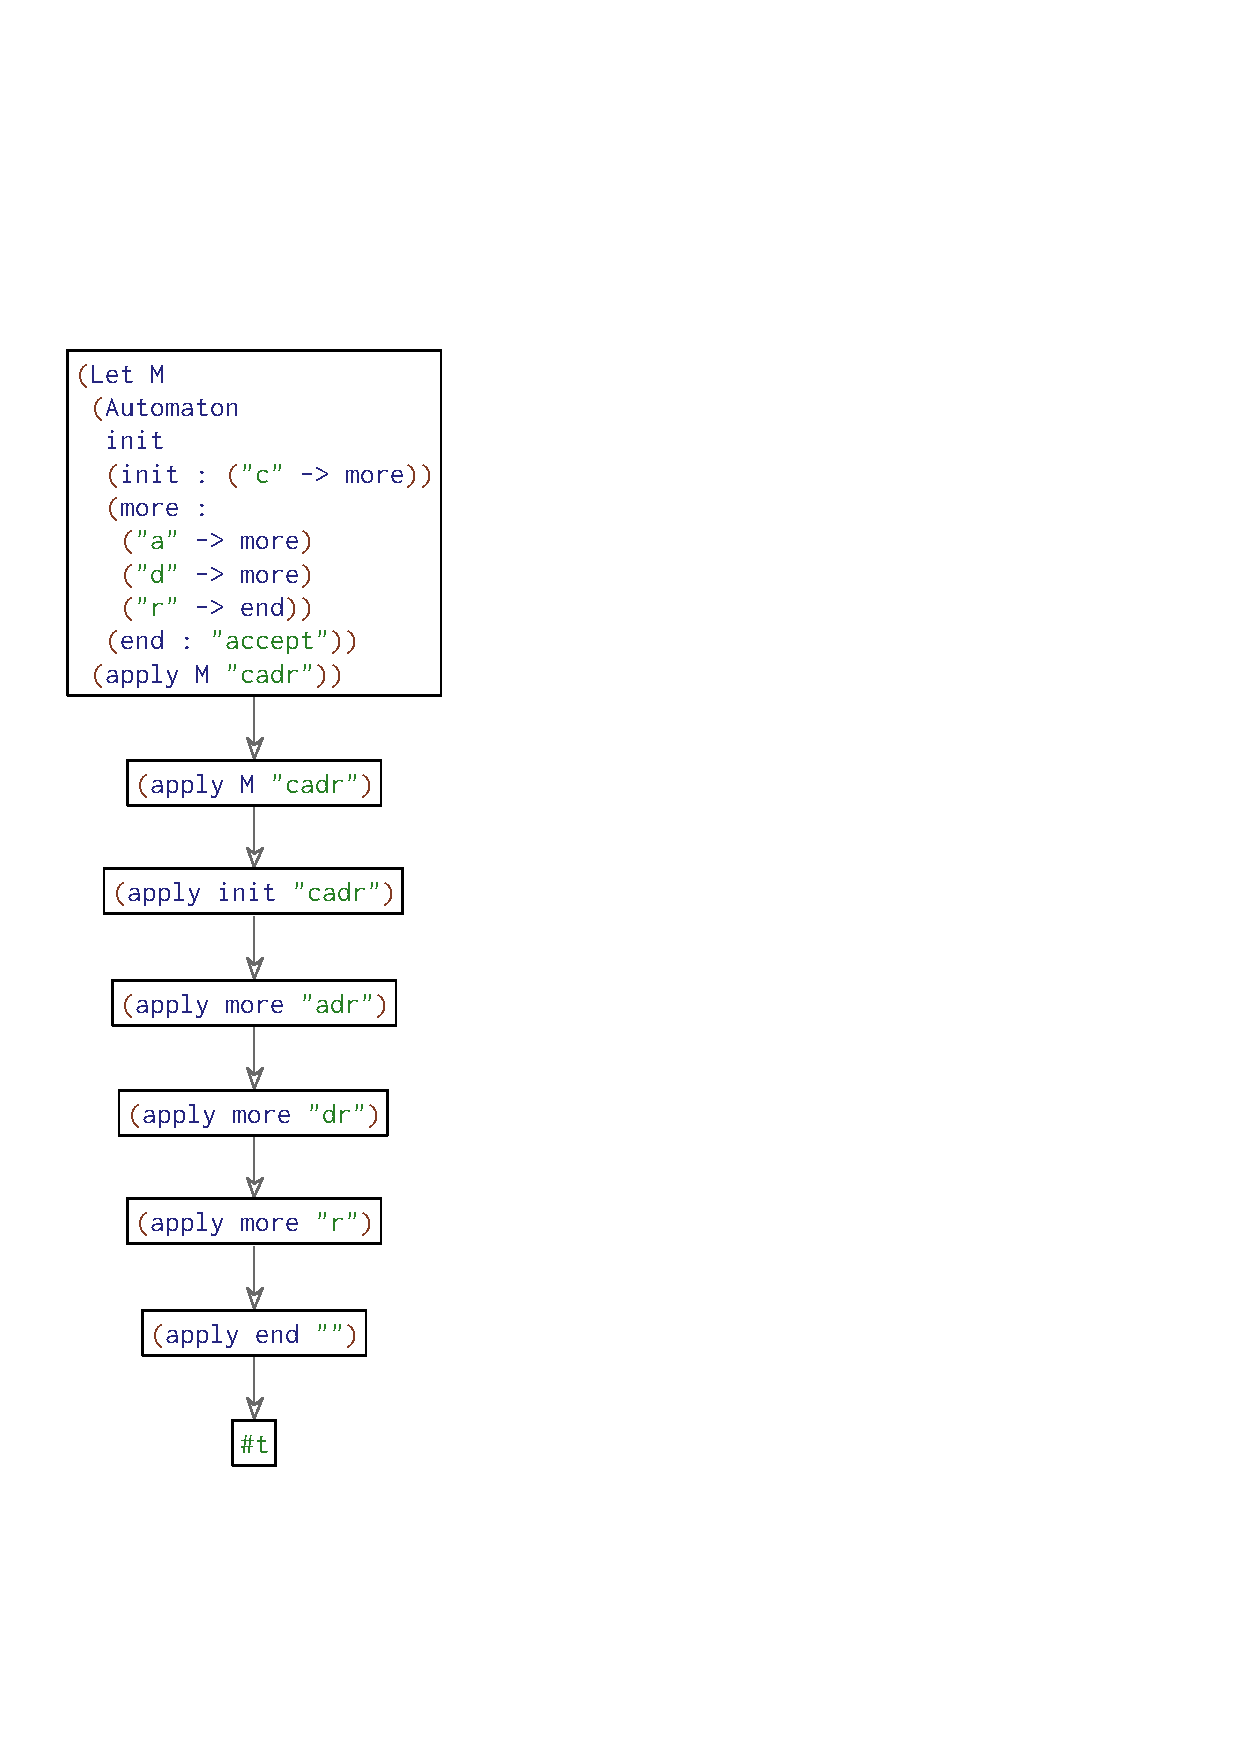
\includegraphics[width=0.45\columnwidth]{automaton-example}\hfill\mbox{}
\caption{Automaton macro execution example}
\label{fig:reval-automaton}
\end{figure}


\subsection{Return}
  Having first-class access to the current continuation is a powerful
  mechanism for defining new control flow constructs. Racket does so with
  the built-in function \Code{call/cc}, that takes a function of one
  argument and calls it with the program's current continuation. Using it,
  we can define a \Code{return} sugar that returns early from a function:
  \begin{codeex}
  Return(x) ->
    Let([Bind("\%RES", x)],
        [Apply(Id("\%RET"), [Id("\%RES")])]);

  Function(args, body) ->
    Lambda(args, Apply(Id("call/cc"),
                       [Lambda(["\%RET"], body)]));
  \end{codeex}
  (The definition of \Code{function} is necessary to mark the point that
  \Code{return} should return to.) With this definition in place, we can
  see evaluation sequences such as:
  \begin{codeex}
    (+ 1 ((function (x) (+ 1 (return (+ x 2)))) (+ 3 4)))
\sstep (+ 1 ((function (x) (+ 1 (return (+ x 2)))) 7))
\sstep (+ 1 (+ 1 (return (+ 7 2))))
\sstep (+ 1 (+ 1 (return 9)))
\sstep (+ 1 9)
\sstep 10
  \end{codeex}
  This example illustrates that our approach is robust enough to work even
  in the presence of dynamic control flow.


\subsection{Pyret: A Case Study}
\label{sec:reval-pyret}

Pyret, shown in \cref{sec:reval-pyret-example}, is a new language. It makes
heavy use of syntactic sugar to emulate the syntax of other programming
languages like Python. This sugar was implemented by people other than
this paper's authors, and written as a manual compiler, not as a set
of rules; it was also implemented without any attention paid to the
limitations of this work. Thus, the language makes for a good case
study for the expressiveness of our work.

We restricted our attention to sugar relevant to evaluation. Pyret has
builtin syntactic forms for writing tests, and can run code both in a
``check'' mode that only runs these tests, or in ``normal'' mode that runs
code. We focused on ``normal'' mode since it is most
relevant to evaluation. There were two pieces of sugar we
were unable to express and one that
required modification to show ideal surface steps; we
describe these in more detail below. 
As \cref{fig:reval-pyretsugar} shows, we were able to handle almost all
of Pyret's sugar. An example of the result in action was shown in
\cref{sec:reval-pyret-example}.

\begin{figure}
\begin{center}\small
\begin{tabular}{l | l c}
  \emph{{\AST} Node} & \emph{Description} & \emph{Implemented?} \\ \hline
  fun & function declaration & yes \\
  when & one-arm conditional & yes \\
  if & multi-arm conditional & yes \\
  cases & multi-arm conditional & yes \\
  cases-else & multi-arm conditional & yes \\
  for & generalized looping construct & yes \\
  op & binary operators & yes \\
  not & negation & yes \\
  paren & grouping construct & yes \\
  left-app & infix notation & yes \\
  list & list expressions & yes \\
  dot & indirect field lookup & yes \\
  colon & direct field lookup & yes \\
  (currying syntax) & allowed in \Code{fun} and \Code{op} & yes \\
\hline
  graph & create cyclic data & no \\
  datatype & datatype declarations & no
\end{tabular}
\end{center}
\caption{Syntactic sugar in normal-mode Pyret}
\label{fig:reval-pyretsugar}
\end{figure}

We were unable to fully handle algebraic datatype declarations
because they splice one block of code into another in a non-compositional
manner; we believe these could be expressed by adding a block
construct that does not introduce a new scope (akin to Scheme's
\Code{begin}).

We were also unable to handle \Code{graph}, which constructs cyclic data.
It has a
complex desugaring that involves creating and updating placeholder values
and compile-time substitution. This could be solved either by expanding
the expressiveness of our system or by adding a new core construct to the
language. There is always a trade-off between the complexity of the core
language and the complexity of the desugaring; when a feature can only be
implemented through a highly non-compositional sugar like this, it may
make sense to instead add the feature to the core language.

Finally, the desugaring for binary operators needed to be modified to show helpful
surface evaluation sequences. The desugaring follows
a strategy similar to that of Python, by applying the \Code{\_plus} method
of the left subexpression to the right subexpression (the \Code{s} terms
are source locations, used for error-reporting):
\begin{codeex}
  Op(s, "+", x, y)  ->
    App(s, Bracket(s, x, Str(s, "_plus")), [y]);
\end{codeex}
Given the term \Code{1 + (2 + 3)}, we would expect evaluation to step
first to \Code{1 + 5} and then to \Code{6}. Unfortunately, {\Resugarer}
shows only this surface evaluation sequence:
\begin{codeex}
    1 + (2 + 3) \ssteparrow 6
\end{codeex}
The core evaluation sequence reveals why:
\begin{codeex}
    1.["_plus"](2.["_plus"](3))
\cstep <func>(2.["_plus"](3))
\cstep <func>(<func>(3))
\cstep <func>(5)
\cstep 6
\end{codeex}
(\Code{<func>} denotes a resolved functional). To show the
term \Code{1 + 5}, Emulation requires that it desugar
precisely into one of the terms in the core sequence; but it desugars
to \Code{1.["\_plus"](5)}, which has a different shape than any of the
core terms.

The fundamental problem is the order of evaluation induced by this
desugaring: first the left subexpression is evaluated, then the
\Code{\_plus} field is resolved, then the right subexpression is
evaluated, then the ``addition'' is performed. We can obtain a more
helpful surface sequence by instead choosing a desugaring
that forces the left and right subexpressions to be evaluated fully before
resolving the operation, as shown in \cref{fig:reval-alt-plus}.

\begin{figure}[t]
\begin{codeex}
  Op(s, "+", x, y) ->
    Block(s,
    [ Let(s, Bind(s, "temp", ABlank),
             Obj(s, [Field(s, Str(s, "left"), x),
                     Field(s, Str(s, "right"), y)]))
    , App(s, Bracket(s, Bracket(s, Id(s, "temp"),
                                   Str(s, "left")),
                        Str(s, "_plus")),
             [Bracket(s, Id(s, "temp"),
                         Str(s, "right"))])]);
\end{codeex}
\caption{Alternate desugaring of addition}
\label{fig:reval-alt-plus}
\end{figure}
This desugaring constructs a temporary object \Code{\{left: x, right:
  y\}}, and then computes \Code{temp.left.\_plus(temp.right)}. Notice that
this desugaring \emph{slightly} changes the semantics of binary operators;
the difference may be seen when the right subexpression mutates the
\Code{\_plus} field of the left subexpression. In exchange, we obtain the
expected surface evaluation sequence:
\begin{codeex}
    1 + (2 + 3) \ssteparrow 1 + 5 \ssteparrow 6
\end{codeex}





\section{Related Work}

There is a long history of trying relate compiled code back to its
source. This problem is especially pronounced in debuggers for
optimizing compilers, where the structure of the source can be altered
significantly~\cite{hennessy-debugging}. Most of this literature
is based on black-box
transformations, unlike ours, which we assume we have full control
over.  As a result, this work tends to be very different in flavor
from ours: some of it is focused on providing high-level
representations of data on the heap, which is a strict subproblem of
ours, or of correlating back to source expression \emph{locations}, which
again is weaker than \emph{reconstructing a source term}.
For this reason,
this work is usually also not accompanied by strong semantic
guarantees or proofs of them.

One line of work in this direction is SELF's debugging
system~\cite{self-debugging}. Its compiler provides its debugger with
debugging information at selected breakpoints by (in part) limiting the
optimizations that are performed around them. This is a sensible approach
when the code transformation in question is optimization and can be turned
off, but does not make sense when the transformation is a desugaring
which is necessary to give the program meaning.

Another line of work in this direction is the compile-time macro error
reporting developed by Culpepper, et al.~\cite{fortifying-macros}.
Constructing useful error messages is a difficult task that we have not
yet addressed. It has a different flavor than the problem we address,
though: akin to previous work in debugging, any source terms mentioned in
an error appear directly in the source, rather than having to be
reconstructed.

Deursen, et al.~\cite{deursen:origin-tracking} formalize the concept of
tracking the origins
of terms within term rewriting systems (which in their case represent
the \emph{evaluator}, not the \emph{syntactic sugar} as in our
case). They go on to show various applications, including
visualizing program execution, implementing debugger breakpoints,
and locating the sources of errors.
Their work does not involve the use of syntactic sugar,
however, while our work hinges on the interplay between syntactic
sugar and evaluation. Nevertheless, we
have adopted their notion of origin tracking for our transformations.

Krishnamurthi, et al.~\cite{sk:mcmicmac} develop a macro system meant
to support a variety of tools, such as type-checkers and
debuggers. Tools can provide feedback to users in terms of the
programmer's source using source locations recorded during
transformation. The system does not, however, reconstruct source
terms; it merely point out relevant parts of the original source.  The
source tracking mechanisms are based on Dybvig, et al.'s macro
system~\cite{expansion-passing-style}.

Clements~\cite[page 53]{clements:thesis} implements an algebraic
stepper (similar to ours) for Racket---a language that has
macros---and thus faces precisely the same problem we address in this
paper. That work, however, side-steps these issues by handling a
certain fixed set of macros specially (those in the ``Beginner
Student'' language) and otherwise showing only expanded code.
On the other hand, it proves that its method of instrumenting a program to
show evaluation steps is correct (i.e., the instrumented program shows the
same evaluation steps that the original program produces),
while we only show that the lifted evaluation sequence is correct
with respect to the core stepper. Thus its approach could be
usefully composed with ours to achieve stronger guarantees.

Fisher and Shivers~\cite{ziggurat} develop a framework
for defining static semantics that connect the
surface and core languages. They show how to effectively \emph{lower}
a \emph{static} semantics from a surface language to its core
language. This is complementary to our work, which
shows how to \emph{lift} a \emph{dynamic} semantics from core to surface.
This exposes a fundamental difference in starting assumptions:
they assume the surface language has a static semantics, while we assume
its semantics is \emph{defined} by desugaring.

In a similiar vein, Lorenzen and Erdweg \cite{typechecking-exts} give a
method for ensuring the type soundness of syntactic extensions by lowering
author-provided typing rules for the surface language onto the core
language's type system (and automatically verifying that soundness is
entailed). Thus their work does for type checking what ours does for
evaluation: it provides a surface type checker guaranteed to be sound with
respect to the core language, while ours produces a surface evaluator
guaranteed to emulate the core language.

Model-driven software engineering also draws heavily on
bidirectional transformation, because systems are expected to be written
in a collection of domain-specific languages that are transformed into
implementations. These uses tend to be \emph{static}, rather
than addressing the inverse-mapping problem in the context of system
execution (see the survey by
Stevens~\cite{bidirectional-model-transfs}).
When the problem we address does arise in this area, it is typically the
case that either (i) both the source and target models have
implementations, so that surface-level execution traces can be obtained
by evaluating in the surface language directly~\cite{Perera-slicing}, or
(ii) the surface information sought is more limited than the reduction
sequence we provide (in the same ways as for debuggers for optimizing
compilers, as described earlier).
Applying our results to this area is future work.

\subsection*{Artifact Evaluation}

The artifact for this paper was not submitted for evaluation because
the second author was a co-chair of the evaluation process. The
artifact is available from
\begin{center}
\url{http://cs.brown.edu/research/plt/dl/resugaring/v1/}
\end{center}

\acks We thank Daniel J.~Dougherty and Matthias Felleisen for their feedback,
Joe Politz for a language that offered an excellent proving ground for
this work, and the anonymous reviewers who provided helpful feedback on
the paper. This work was partially supported by support from the US
National Science Foundation and Google.

\bibliography{justin}
\bibliographystyle{terseabbrvnat}

\end{document}

%\chapter{Resugaring Scope}\label{chap:resugar-scope}

\section{Scope Checking}

(See \cref{fig:scope}.)

\begin{figure}
\TypeLabel{\SaysScope{\Sigma}{e}
  {\{\Decl{x}\}}
  {\{\Refn{x}\}}
  {\{\Decl{x}\}}
  {\{\Refn{x}\mapsto\Decl{x}\}}}

\Inference[scope-e-decl]{}{
  \SaysScope{\Sigma}{\Decl{x}}{\{\Decl{x}\}}{\{\}}{\{\Decl{x}\}}{\{\}}
}

\Inference[scope-e-refn]{}{
  \SaysScope{\Sigma}{\Refn{x}}{\{\}}{\{\Refn{x}\}}{\{\}}{\{\}}
}

\Inference[scope-e-con]{
  \Sigma[C] = \sigma \vspace{0.1em} \IS\\
  \SaysScope{\Sigma}{e_i}{P_i}{R_i}{B_i} \text{ for } i \in 1..n \IS\\
  S = \SetSuchThat{
    \Decl[a]{x} \mapsto \Decl[b]{x}
  }{
    \Decl[a]{x} \in P_i,\;
    \Decl[b]{x} \in P_j,\;
    \Bind{\sigma}{i}{j}
  } \IS\\
  B = \SetSuchThat{
    \Refn[a]{x} \mapsto \Decl[b]{x}
  }{
    \Refn[a]{x} \in R_i,\;
    \Decl[b]{x} \in P_j,\;
    \Bind{\sigma}{i}{j},\;
    \Decl[b]{x} \not\in \Domain{S}
  } \IS\\
  R = \SetSuchThat{
    \Refn[a]{x}
  }{
    \Refn[a]{x} \in R_i,\;
    \NotExists{\Decl[b]{x}}{\Refn[a]{x} \mapsto \Decl[b]{x} \in B\}}
  } \IS\\
  P = \SetSuchThat{
    \Decl[a]{x}
  }{
    \Decl[a]{x} \in P_i,\;
    \Prov{\sigma}{i},\;
    \Decl[a]{x} \not\in \Domain{S}
  }
}{
  \SaysScope{\Sigma}{\Core{C}{e_1 ... e_n}}{P}{R}{B}
}


\Inference[scope-p-con]{
  \Sigma[C] = \sigma \vspace{0.1em} \IS\\
  \SaysScope{\Sigma}{p_i}{P_i}{R_i}{B_i} \text{ for } i \in 1..n \IS\\
  S = \SetSuchThat{
    a \mapsto b
  }{
    a \in P_i,\;
    b \in P_j,\;
    \Bind{\sigma}{i}{j},\;
    \SaysCanShadow{F}{a}{b}
  } \IS\\
  B = \SetSuchThat{
    a \mapsto b
  }{
    a \in R_i,\;
    b \in P_j,\;
    \Bind{\sigma}{i}{j},\;
    b \not\in \Domain{S},\;
    \SaysCanBind{F}{a}{b}
  } \IS\\
  R = \SetSuchThat{
    a
  }{
    a \in R_i,\;
    (\NotExists{b}{a \mapsto b \in B\}}
    \text{ or $a$ is a pattern var})
  } \IS\\
  P = \SetSuchThat{
    a
  }{
    a \in P_i,\;
    \Prov{\sigma}{i},\;
    a \not\in \Domain{S}
  }
}{
  \SaysScope{\Sigma}{\Core{C}{p_1 ... p_n}}{P}{R}{B}
}

Two checks to make: fresh vars don't bind to non-fresh vars, and named
vars only bind to vars of the same name:
\begin{multicols}{3}
  \Inference{}{
    \SaysCanBind{F}{\Refn[1]{x}}{\Decl[2]{x}}
  }
  \Inference{
    x \not\in F
  }{
    \SaysCanBind{F}{\Refn[1]{x}}{\PVarA}
  }
  \Inference{
    x \not\in F
  }{
    \SaysCanBind{F}{\PVarA}{\Decl[1]{x}}
  }
  \Inference{}{
    \SaysCanBind{F}{\PVarA}{\PVarB}
  }
  \Inference{}{
    \SaysCanShadow{F}{\Decl[1]{x}}{\Decl[2]{x}}
  }
  \Inference{
    x \not\in F
  }{
    \SaysCanShadow{F}{\Decl[1]{x}}{\PVarA}
  }
\end{multicols}

\caption{Scope Checking Rules}
\label{fig:scope}
\end{figure}

%\chapter{Resugaring Types}\label{chap:resugar-type}

TODO
\begin{itemize}
\item Update: section 3.1, desugaring definition
\item Update: section 4.2, ``will only ever be bound to surface terms''
\item Update: section 4.3, capturing set
\item RW: ``restoring the adage'' - put in introduction
\end{itemize}

% Chapter: Implementation
% Chapter: Conclusion/future work





\chapter{Appendix}


% Expressions & Grammars
\newcommand{\lit}[1]{\textbf{#1}}
\newcommand{\expr}[2]{(#1\,#2)}
\newcommand{\var}[1]{\textrm{\textsc{#1}}}

% Grammars
\newcommand{\exprs}[3]{(#1\,#2\,#3^{*})}
\newcommand{\production}[2]{#1 \leftarrow #2}
\newcommand{\saysG}[3]{#1 \vdash #2\,:\,#3}

% Scope
\newcommand{\SaysScopeCheck}[6]{#1 \vdash #2 : #3 ; #4 ; #5 ; #6}


\subsection{Terms}

We will call \textsc{ast} terms \emph{expressions} and write them in
s-expression form. Atomic terms are either variables or literals
(i.e. syntactic constants), and compound terms are built with
\emph{term constructors} $P$:

\begin{Table}
  $e$
  &$::=$& $\lit{lit}$ &(literal) \\
  &$|$&   $\var{x}$ &(variable) \\
  &$|$&   $\expr{P}{e_1 ... e_n}$ &(\textsc{ast} node)
\end{Table}

\subsection{Tree Grammars}

A \emph{tree grammar} [CITE] is to trees as a context-free grammar is
to strings. Thus it can be viewed either as a set of instructions for
how to iteratively and nondeterministically rewrite a starting
\emph{nonterminal} to a final tree; \emph{or} it can be viewed as a
specification of a grammar that a tree may or may not follow. We will
take the latter view.

Definitionally, a tree grammar consists of a number of
\emph{productions} that map \emph{nonterminals} $s$ to
\emph{patterns}:
\begin{Table}
  $G$
  &$::=$& $\left\{ \begin{array}{l}
    \production{s_1}{\emph{pattern}_1} \\
    \ddd \\
    \production{s_n}{\emph{pattern}_n}
    \end{array}\right.$ \\
  \\
  $\emph{pattern}$
  &$::=$& $\expr{P}{s_1 \dd s_n}$ &(regular pattern) \\
  &$|$&
  $\exprs{P}{s_1 \dd s_n}{s_{n+1}}$
  &(ellipses pattern) \\
  &$|$&   $\emph{literal}$ &(matches literals) \\
  &$|$&   $\emph{var}$ &(matches variables)
\end{Table}

The \emph{meaning} of a tree grammar (again, we are viewing the
grammar as a \emph{specification}) is that for each production
``$\production{s}{\emph{pattern}}$'', if a term matches the
\emph{pattern}, then it also matches the nonterminal $s$. Formally:

\[
\fbox{$\saysG{G}{e}{s}$}
\]

\[
\inference
    [G-literal]
    {}
    {\saysG{G}{\lit{lit}}{\emph{literal}}}
\quad
\inference
    [G-variable]
    {}
    {\saysG{G}{\var{x}}{\emph{variable}}}
\]
    
\[
\inference
    [G-node]
    {\Forall{i \in 1..n} \saysG{G}{e_i}{s_i} \\
      \production{s}{\expr{P}{s_1 \dd s_n}} \in G}
    {\saysG{G}{\expr{P}{e_1 \dd e_n}}{s}}
\quad
\inference
    [G-ellipses]
    {\Forall{i \in 1..n} \saysG{G}{e_i}{s_i} \\
      \Forall{j \in 1..k} \saysG{G}{e_{n+j}}{s} \\
      \production{s}{\exprs{P}{s_1 \dd s_n}{s}} \in G}
    {\saysG{G}{\expr{P}{e_1 \dd e_n \dd e_{n+k}}}{s}}
\]


\section{Scope Checking}

(See \cref{fig:scope}.)

\begin{figure}
\TypeLabel{\SaysScopeCheck{\Sigma}{e}
  {\{\Decl{x}\}}
  {\{\Refn{x}\}}
  {\{\Decl{x}\}}
  {\{\Refn{x}\mapsto\Decl{x}\}}}

\Inference[scope-e-decl]{}{
  \SaysScopeCheck{\Sigma}{\Decl{x}}{\{\Decl{x}\}}{\{\}}{\{\Decl{x}\}}{\{\}}
}

\Inference[scope-e-refn]{}{
  \SaysScopeCheck{\Sigma}{\Refn{x}}{\{\}}{\{\Refn{x}\}}{\{\}}{\{\}}
}

\Inference[scope-e-con]{
  \Sigma[C] = \sigma \vspace{0.1em} \IS\\
  \SaysScopeCheck{\Sigma}{e_i}{P_i}{R_i}{B_i} \text{ for } i \in 1..n \IS\\
  S = \SetSuchThat{
    \Decl[a]{x} \mapsto \Decl[b]{x}
  }{
    \Decl[a]{x} \in P_i,\;
    \Decl[b]{x} \in P_j,\;
    \Bind{\sigma}{i}{j}
  } \IS\\
  B = \SetSuchThat{
    \Refn[a]{x} \mapsto \Decl[b]{x}
  }{
    \Refn[a]{x} \in R_i,\;
    \Decl[b]{x} \in P_j,\;
    \Bind{\sigma}{i}{j},\;
    \Decl[b]{x} \not\in \Domain{S}
  } \IS\\
  R = \SetSuchThat{
    \Refn[a]{x}
  }{
    \Refn[a]{x} \in R_i,\;
    \NotExists{\Decl[b]{x}}{\Refn[a]{x} \mapsto \Decl[b]{x} \in B\}}
  } \IS\\
  P = \SetSuchThat{
    \Decl[a]{x}
  }{
    \Decl[a]{x} \in P_i,\;
    \Prov{\sigma}{i},\;
    \Decl[a]{x} \not\in \Domain{S}
  }
}{
  \SaysScopeCheck{\Sigma}{\Core{C}{e_1 ... e_n}}{P}{R}{B \cup B_1 \cup \ddd \cup B_n}
}


\Inference[scope-p-con]{
  \Sigma[C] = \sigma \vspace{0.1em} \IS\\
  \SaysScopeCheck{\Sigma}{p_i}{P_i}{R_i}{B_i} \text{ for } i \in 1..n \IS\\
  S = \SetSuchThat{
    a \mapsto b
  }{
    a \in P_i,\;
    b \in P_j,\;
    \Bind{\sigma}{i}{j},\;
    \SaysCanShadow{F}{a}{b}
  } \IS\\
  B = \SetSuchThat{
    a \mapsto b
  }{
    a \in R_i,\;
    b \in P_j,\;
    \Bind{\sigma}{i}{j},\;
    b \not\in \Domain{S},\;
    \SaysCanBind{F}{a}{b}
  } \IS\\
  R = \SetSuchThat{
    a
  }{
    a \in R_i,\;
    (\NotExists{b}{a \mapsto b \in B\}}
    \text{ or $a$ is a pattern var})
  } \IS\\
  P = \SetSuchThat{
    a
  }{
    a \in P_i,\;
    \Prov{\sigma}{i},\;
    a \not\in \Domain{S}
  }
}{
  \SaysScopeCheck{\Sigma}{\Core{C}{p_1 ... p_n}}{P}{R}{B \cup B_1 \cup \ddd \cup B_n}
}

Two checks to make: fresh vars don't bind to non-fresh vars, and named
vars only bind to vars of the same name:
\begin{multicols}{3}
  \Inference{}{
    \SaysCanBind{F}{\Refn[1]{x}}{\Decl[2]{x}}
  }
  \Inference{
    x \not\in F
  }{
    \SaysCanBind{F}{\Refn[1]{x}}{\PVarA}
  }
  \Inference{
    x \not\in F
  }{
    \SaysCanBind{F}{\PVarA}{\Decl[1]{x}}
  }
  \Inference{}{
    \SaysCanBind{F}{\PVarA}{\PVarB}
  }
  \Inference{}{
    \SaysCanShadow{F}{\Decl[1]{x}}{\Decl[2]{x}}
  }
  \Inference{
    x \not\in F
  }{
    \SaysCanShadow{F}{\Decl[1]{x}}{\PVarA}
  }
\end{multicols}

\caption{Scope Checking Rules}
\label{fig:scope}
\end{figure}

\bibliographystyle{plain}
\bibliography{justin}

\end{document}
